\chapter{Parameter Values Distributions in Terms of Contract Violations}\label{appendix:Distributions2}
\begin{figure}
	\centering
	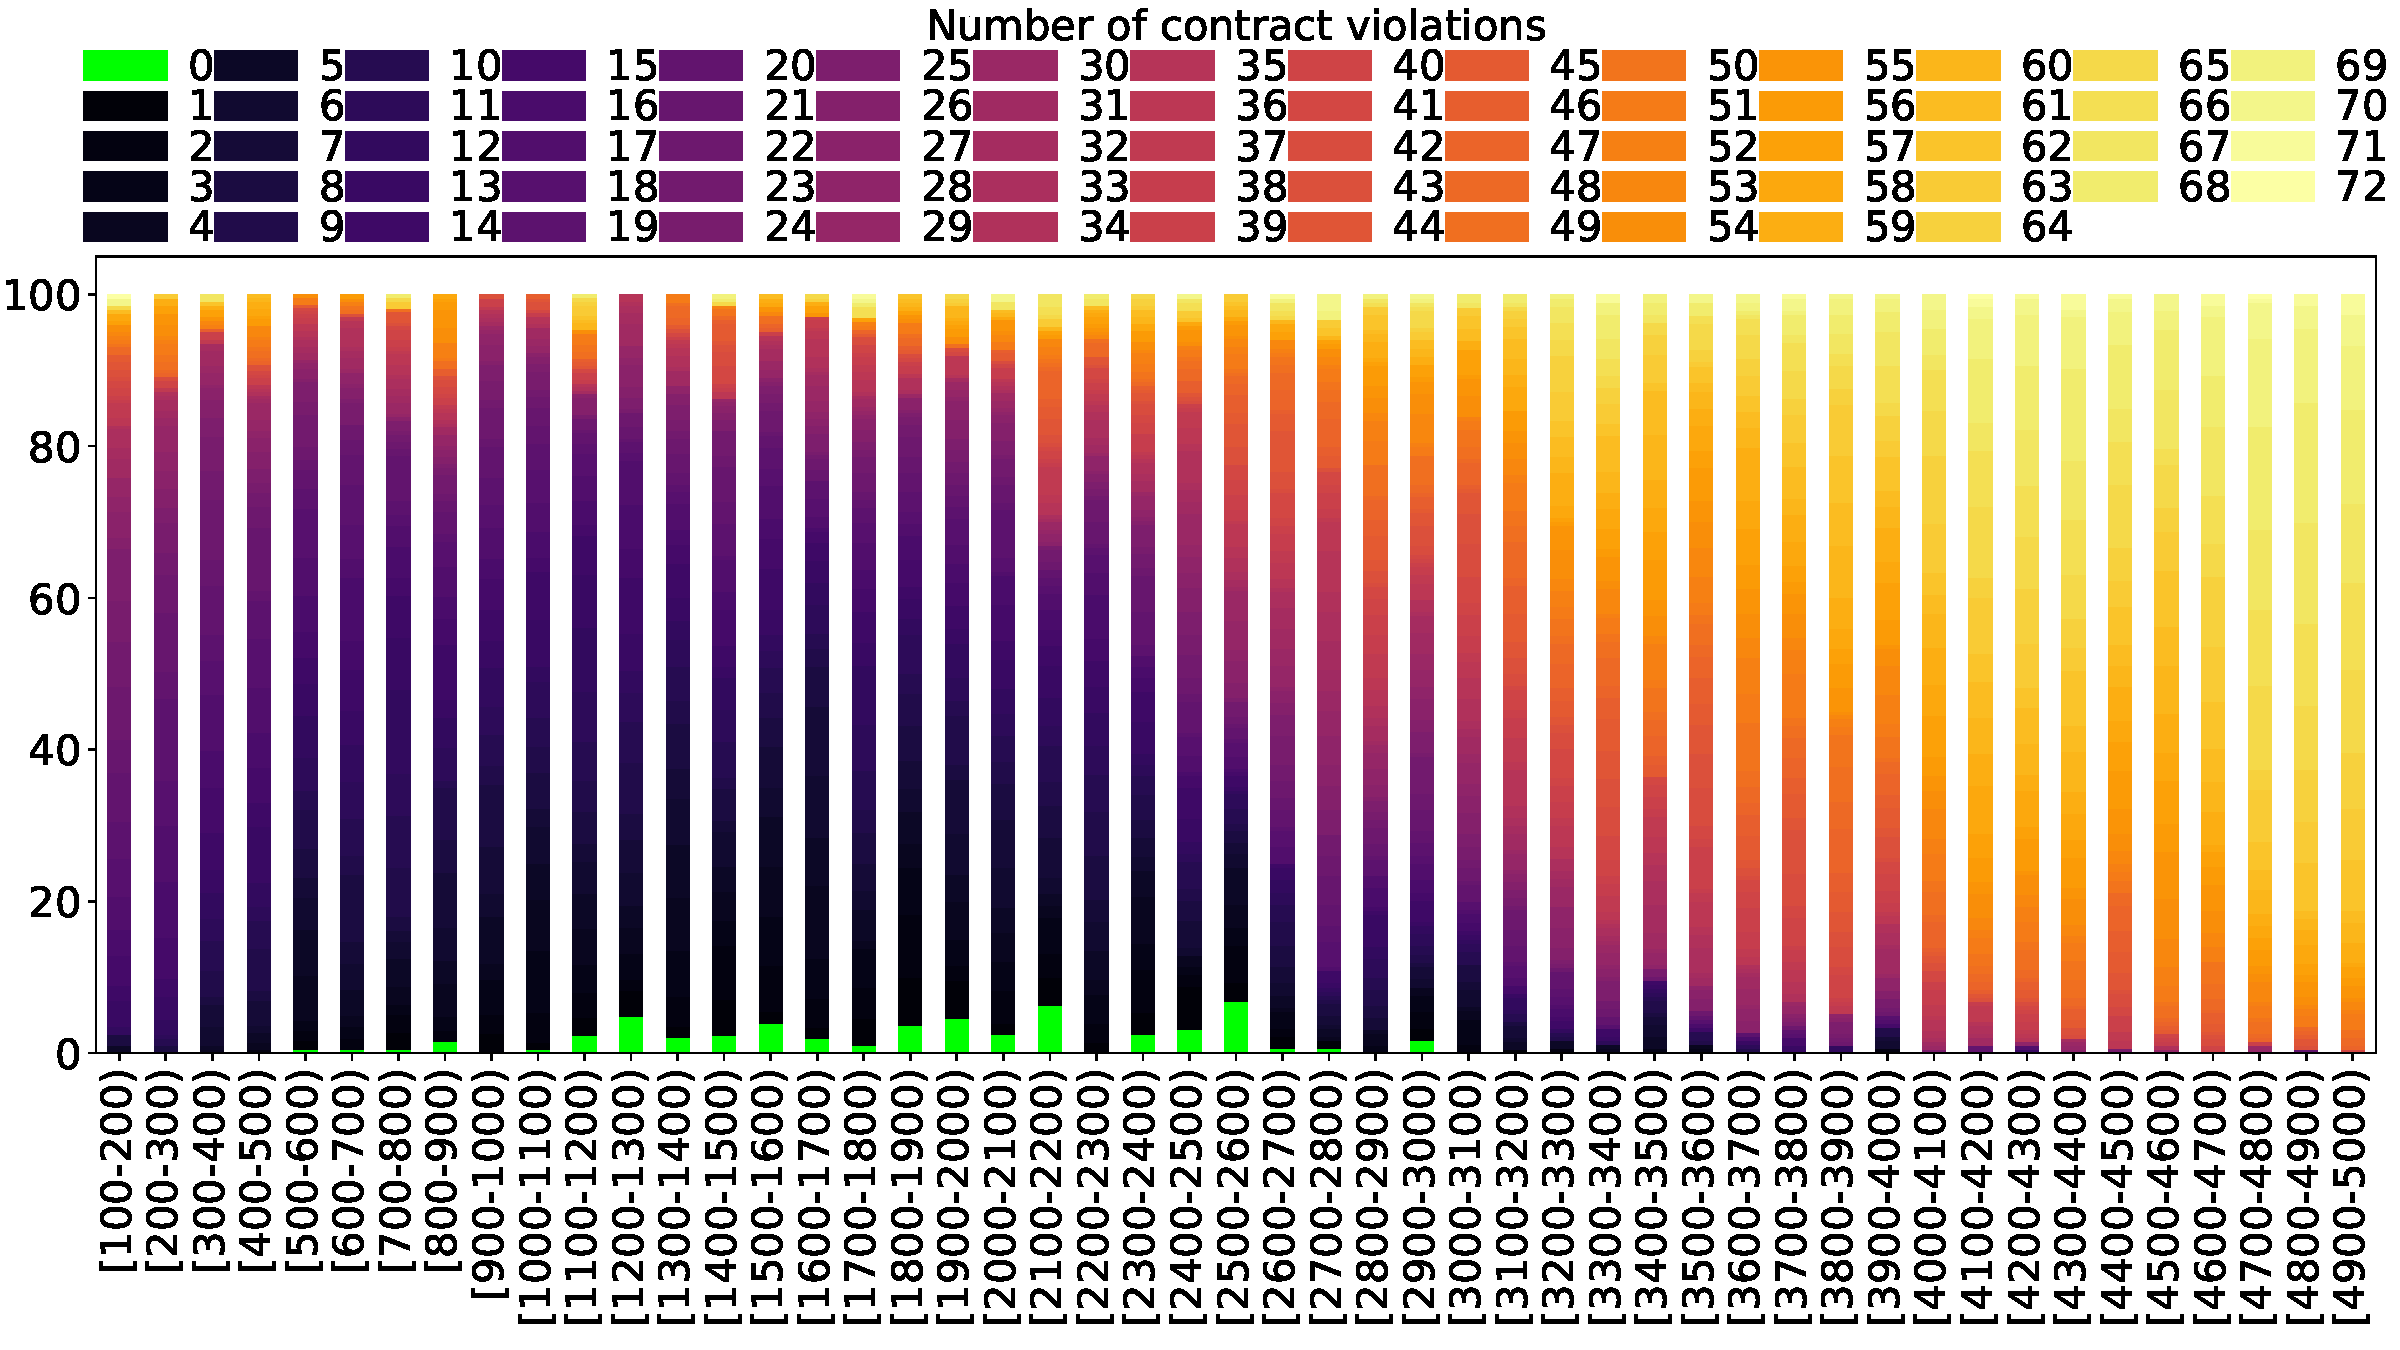
\includegraphics[width=\textwidth]{images/DistrValidityBig/populationSize.pdf}
	\caption[populationSize parameter values distribution for bigger problem]{populationSize parameter values distribution for bigger problem}  
	\label{fig:populationSize_DistBig}
\end{figure}
\begin{figure}
	\centering
	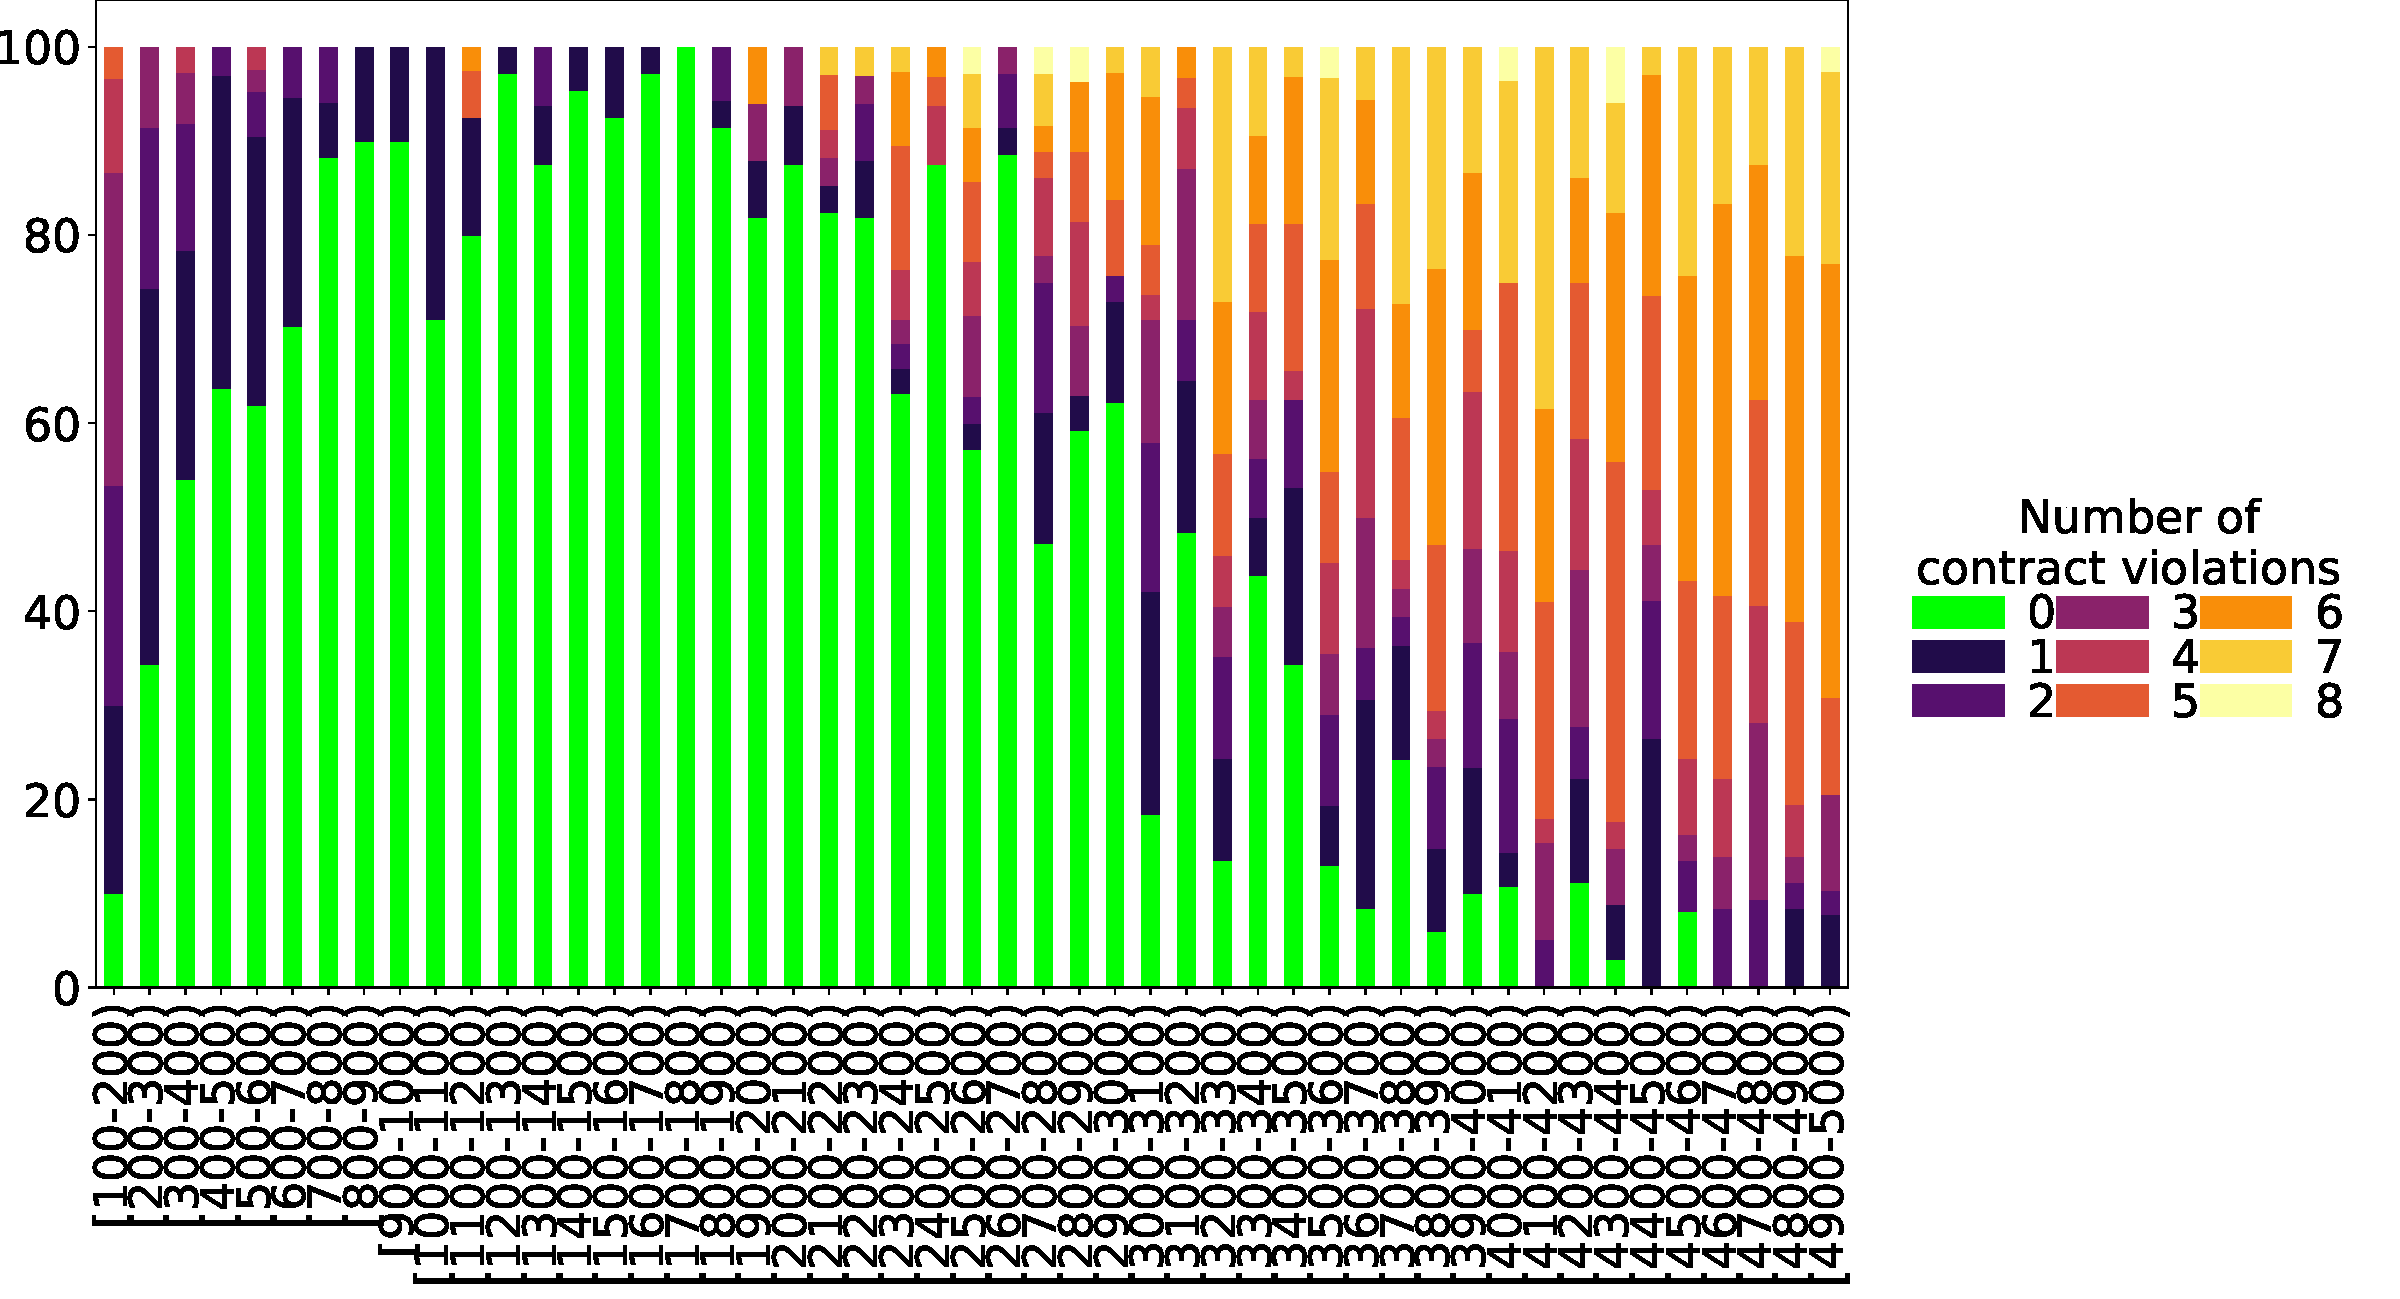
\includegraphics[width=\textwidth]{images/DistrValiditySmall/populationSize.pdf}
	\caption[populationSize parameter values distribution for smaller problem]{populationSize parameter values distribution for smaller problem}
	\label{fig:populationSize_DistSmall}
\end{figure}
\begin{figure}
	\centering
	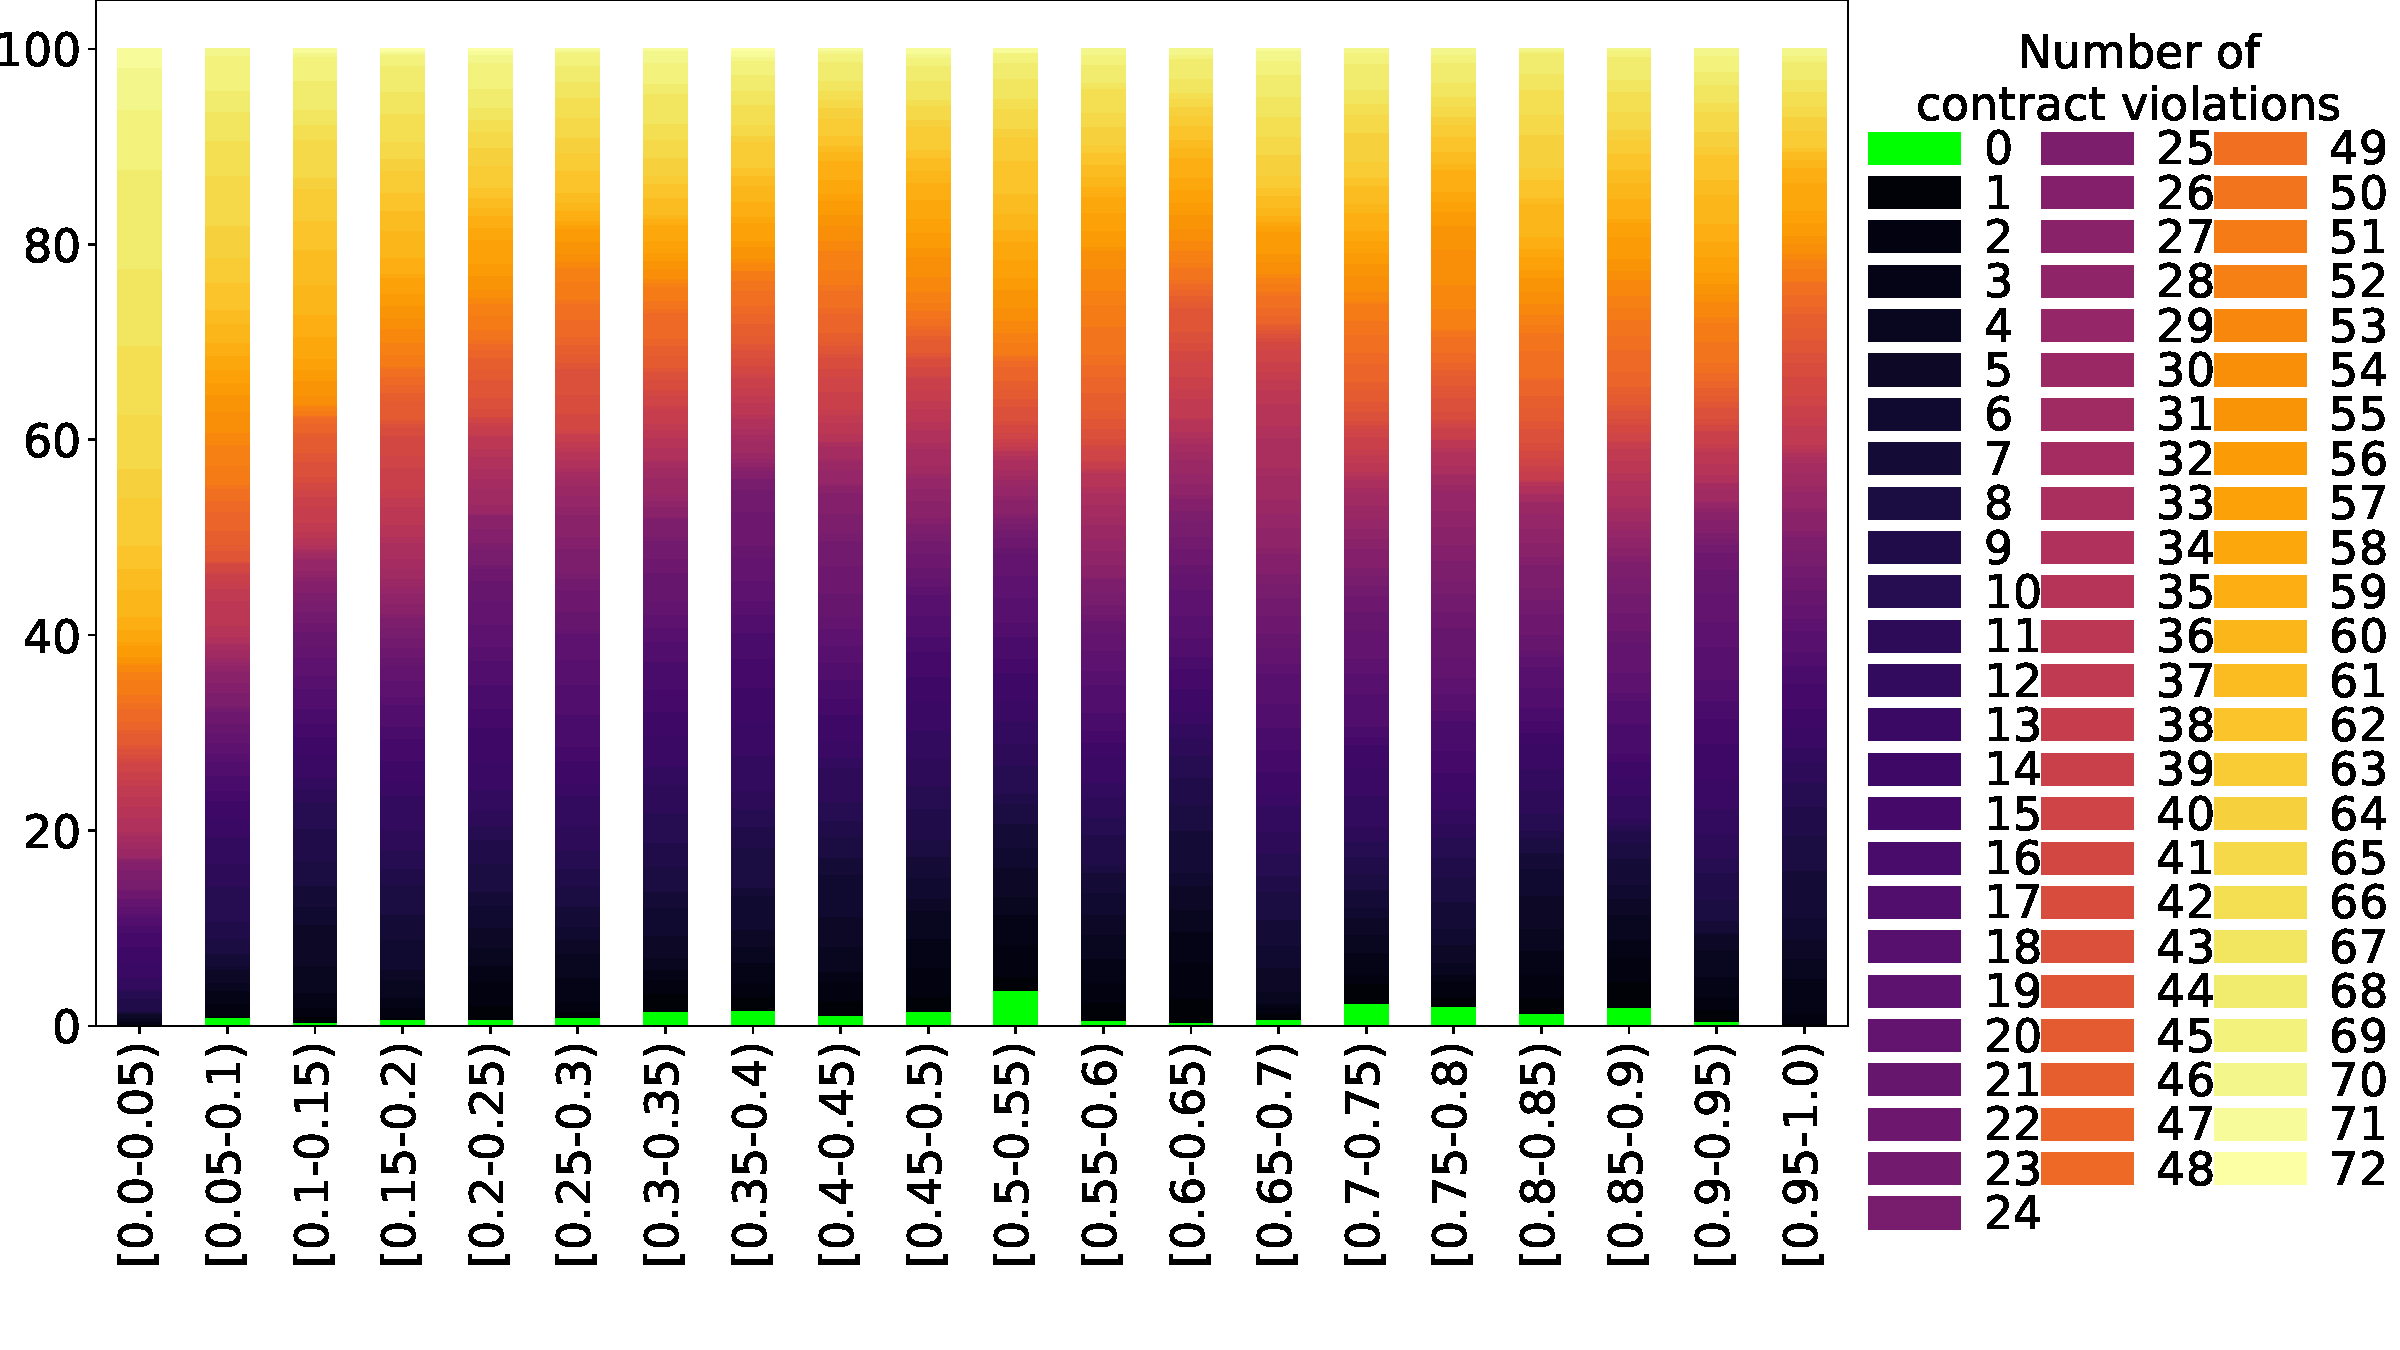
\includegraphics[width=\textwidth]{images/DistrValidityBig/lambda.pdf}
	\caption[lambda parameter values distribution for bigger problem]{lambda parameter values distribution for bigger problem}
	\label{fig:lambda_DistBig}
\end{figure}
\begin{figure}
	\centering
	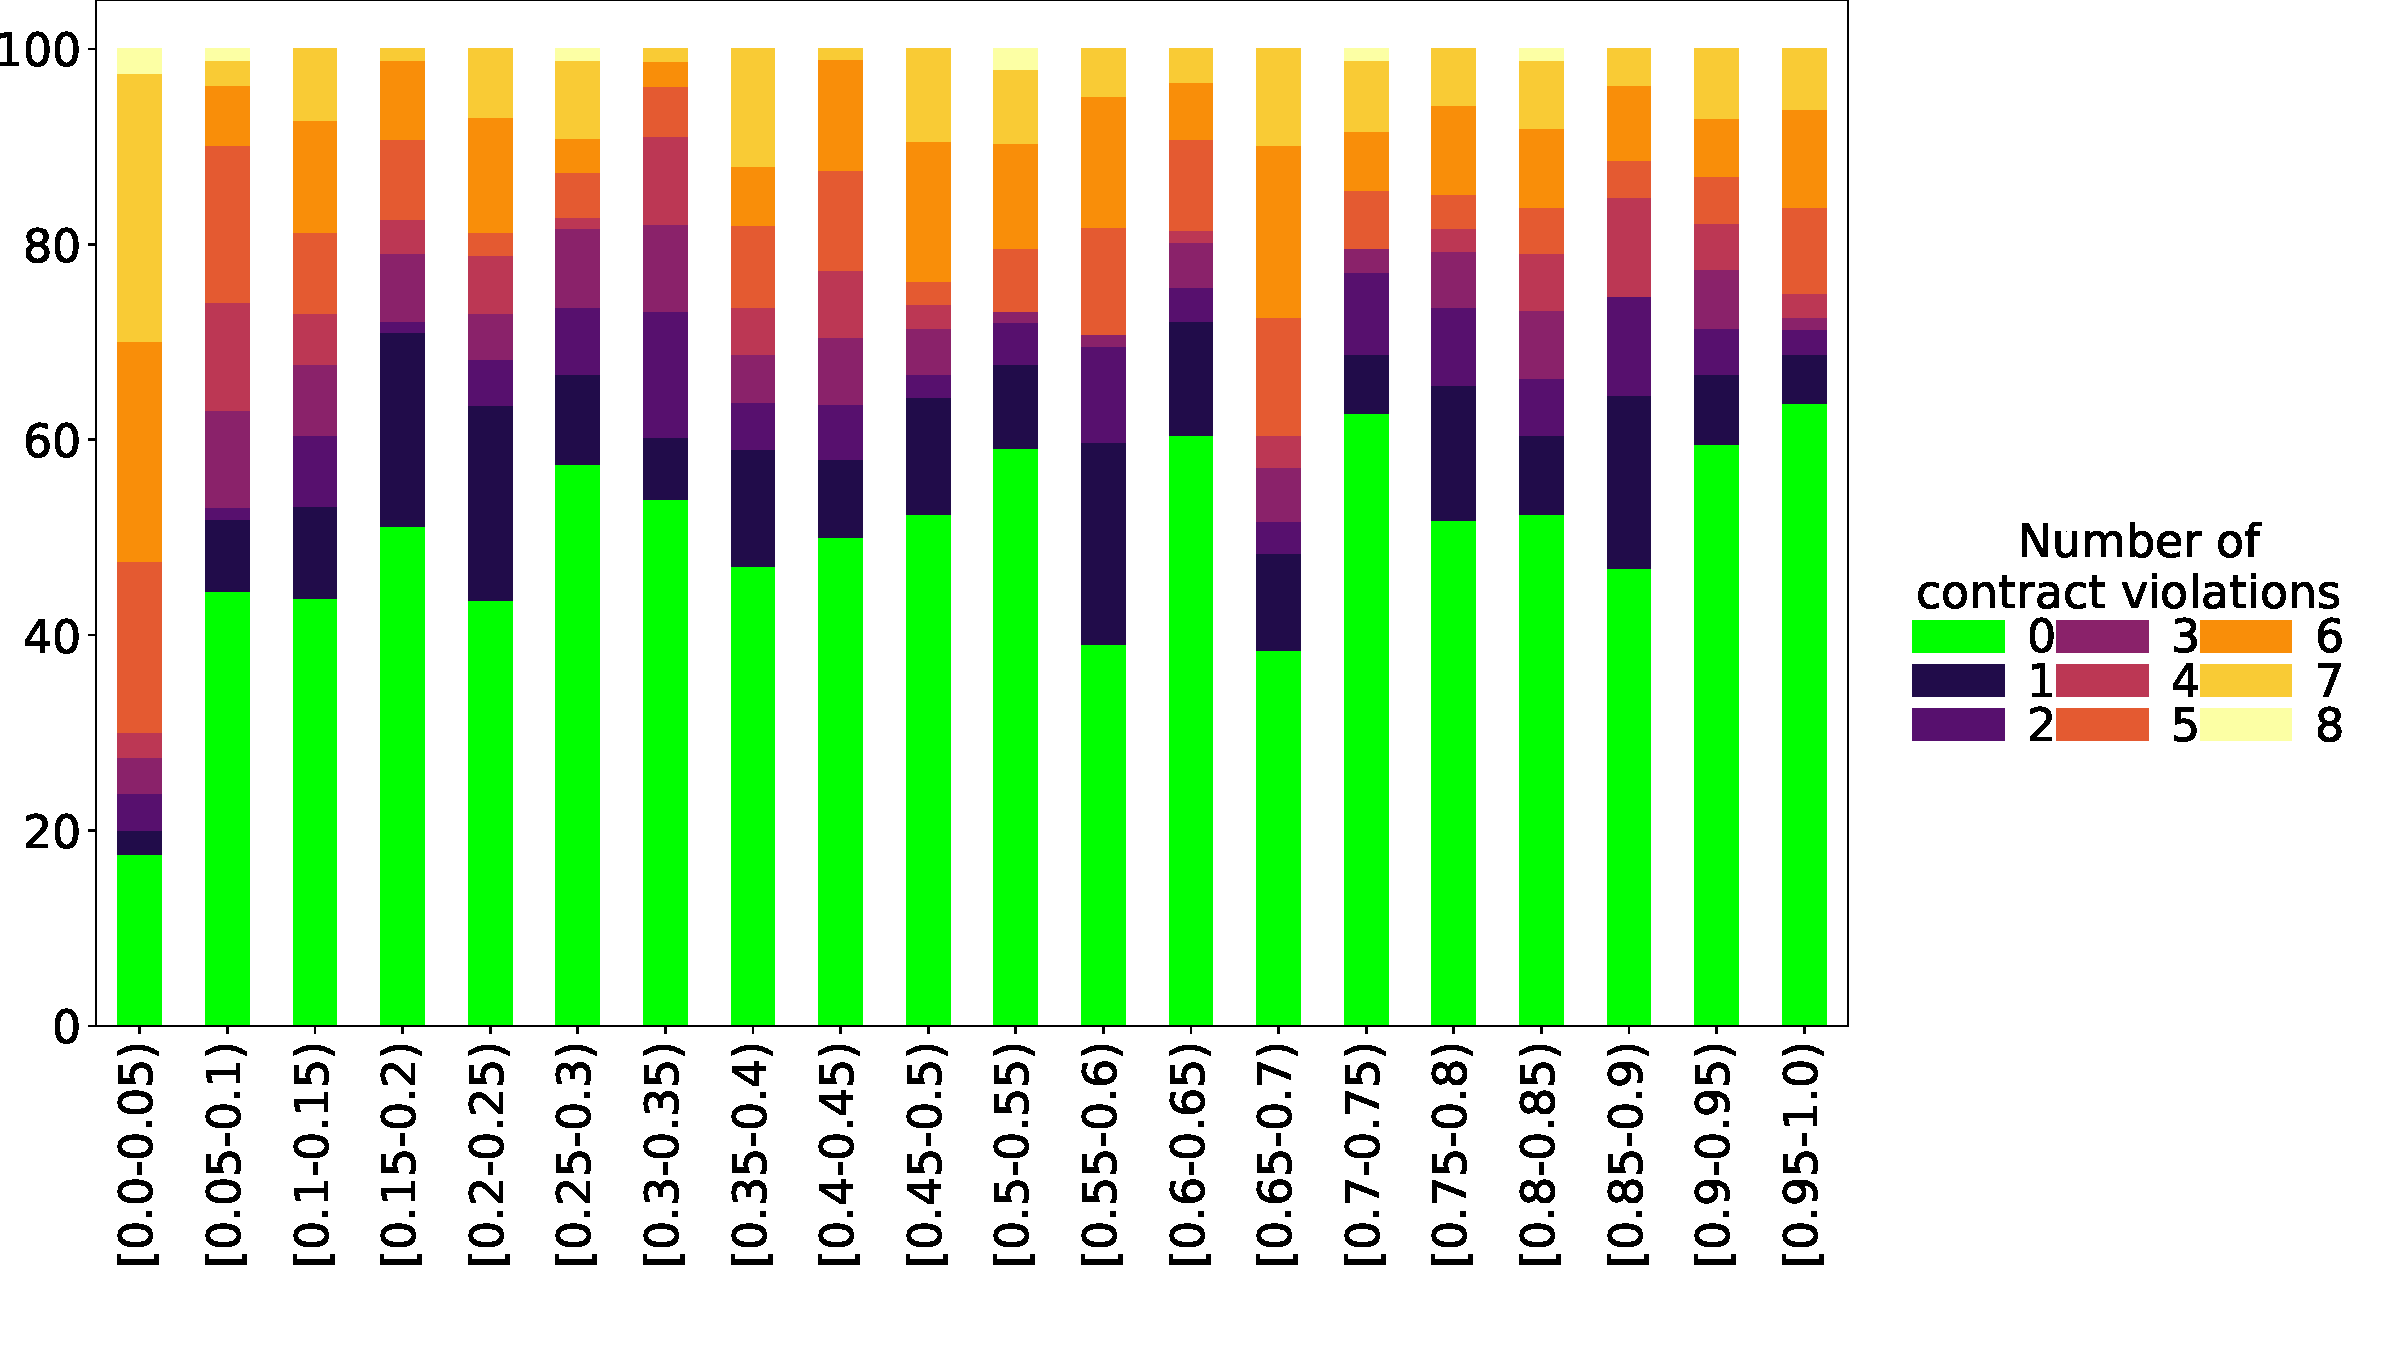
\includegraphics[width=\textwidth]{images/DistrValiditySmall/lambda.pdf}
	\caption[lambda parameter values distribution for smaller problem]{lambda parameter values distribution for smaller problem}
	\label{fig:lambda_DistSmall}
\end{figure}
\begin{figure}
	\centering
	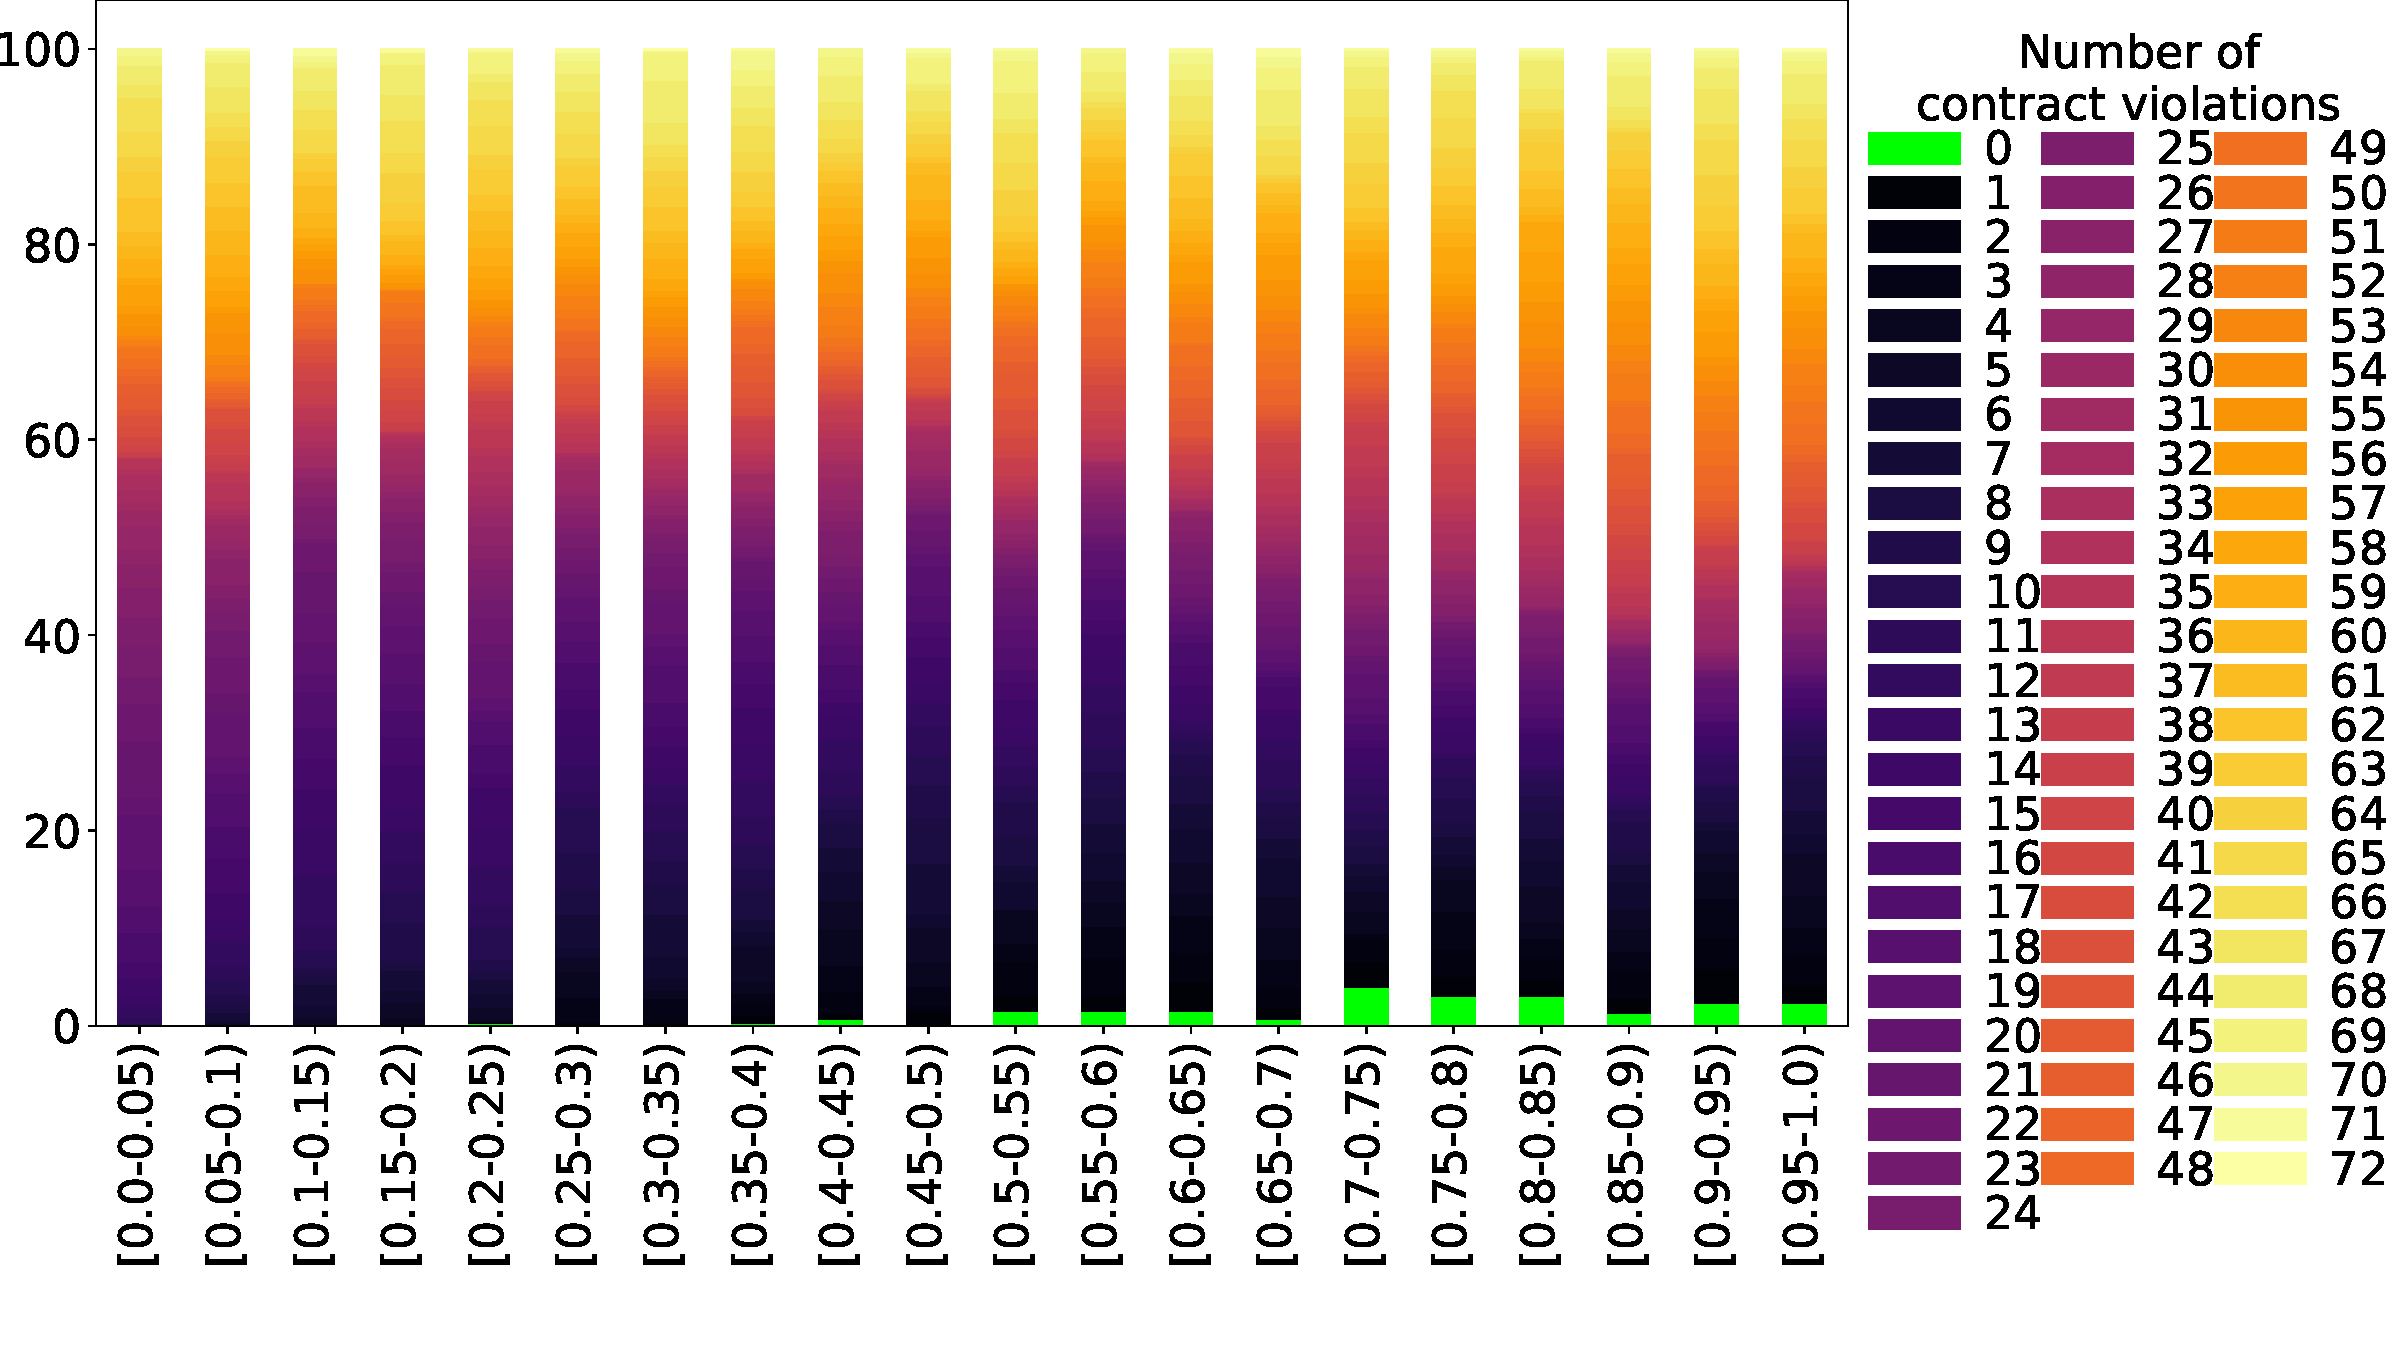
\includegraphics[width=\textwidth]{images/DistrValidityBig/crossoverRate.pdf}
	\caption[crossoverRate parameter values distribution for bigger problem]{crossoverRate parameter values distribution for bigger problem}
	\label{fig:crossoverRate_DistBig}
\end{figure}
\clearpage
\begin{figure}
	\centering
	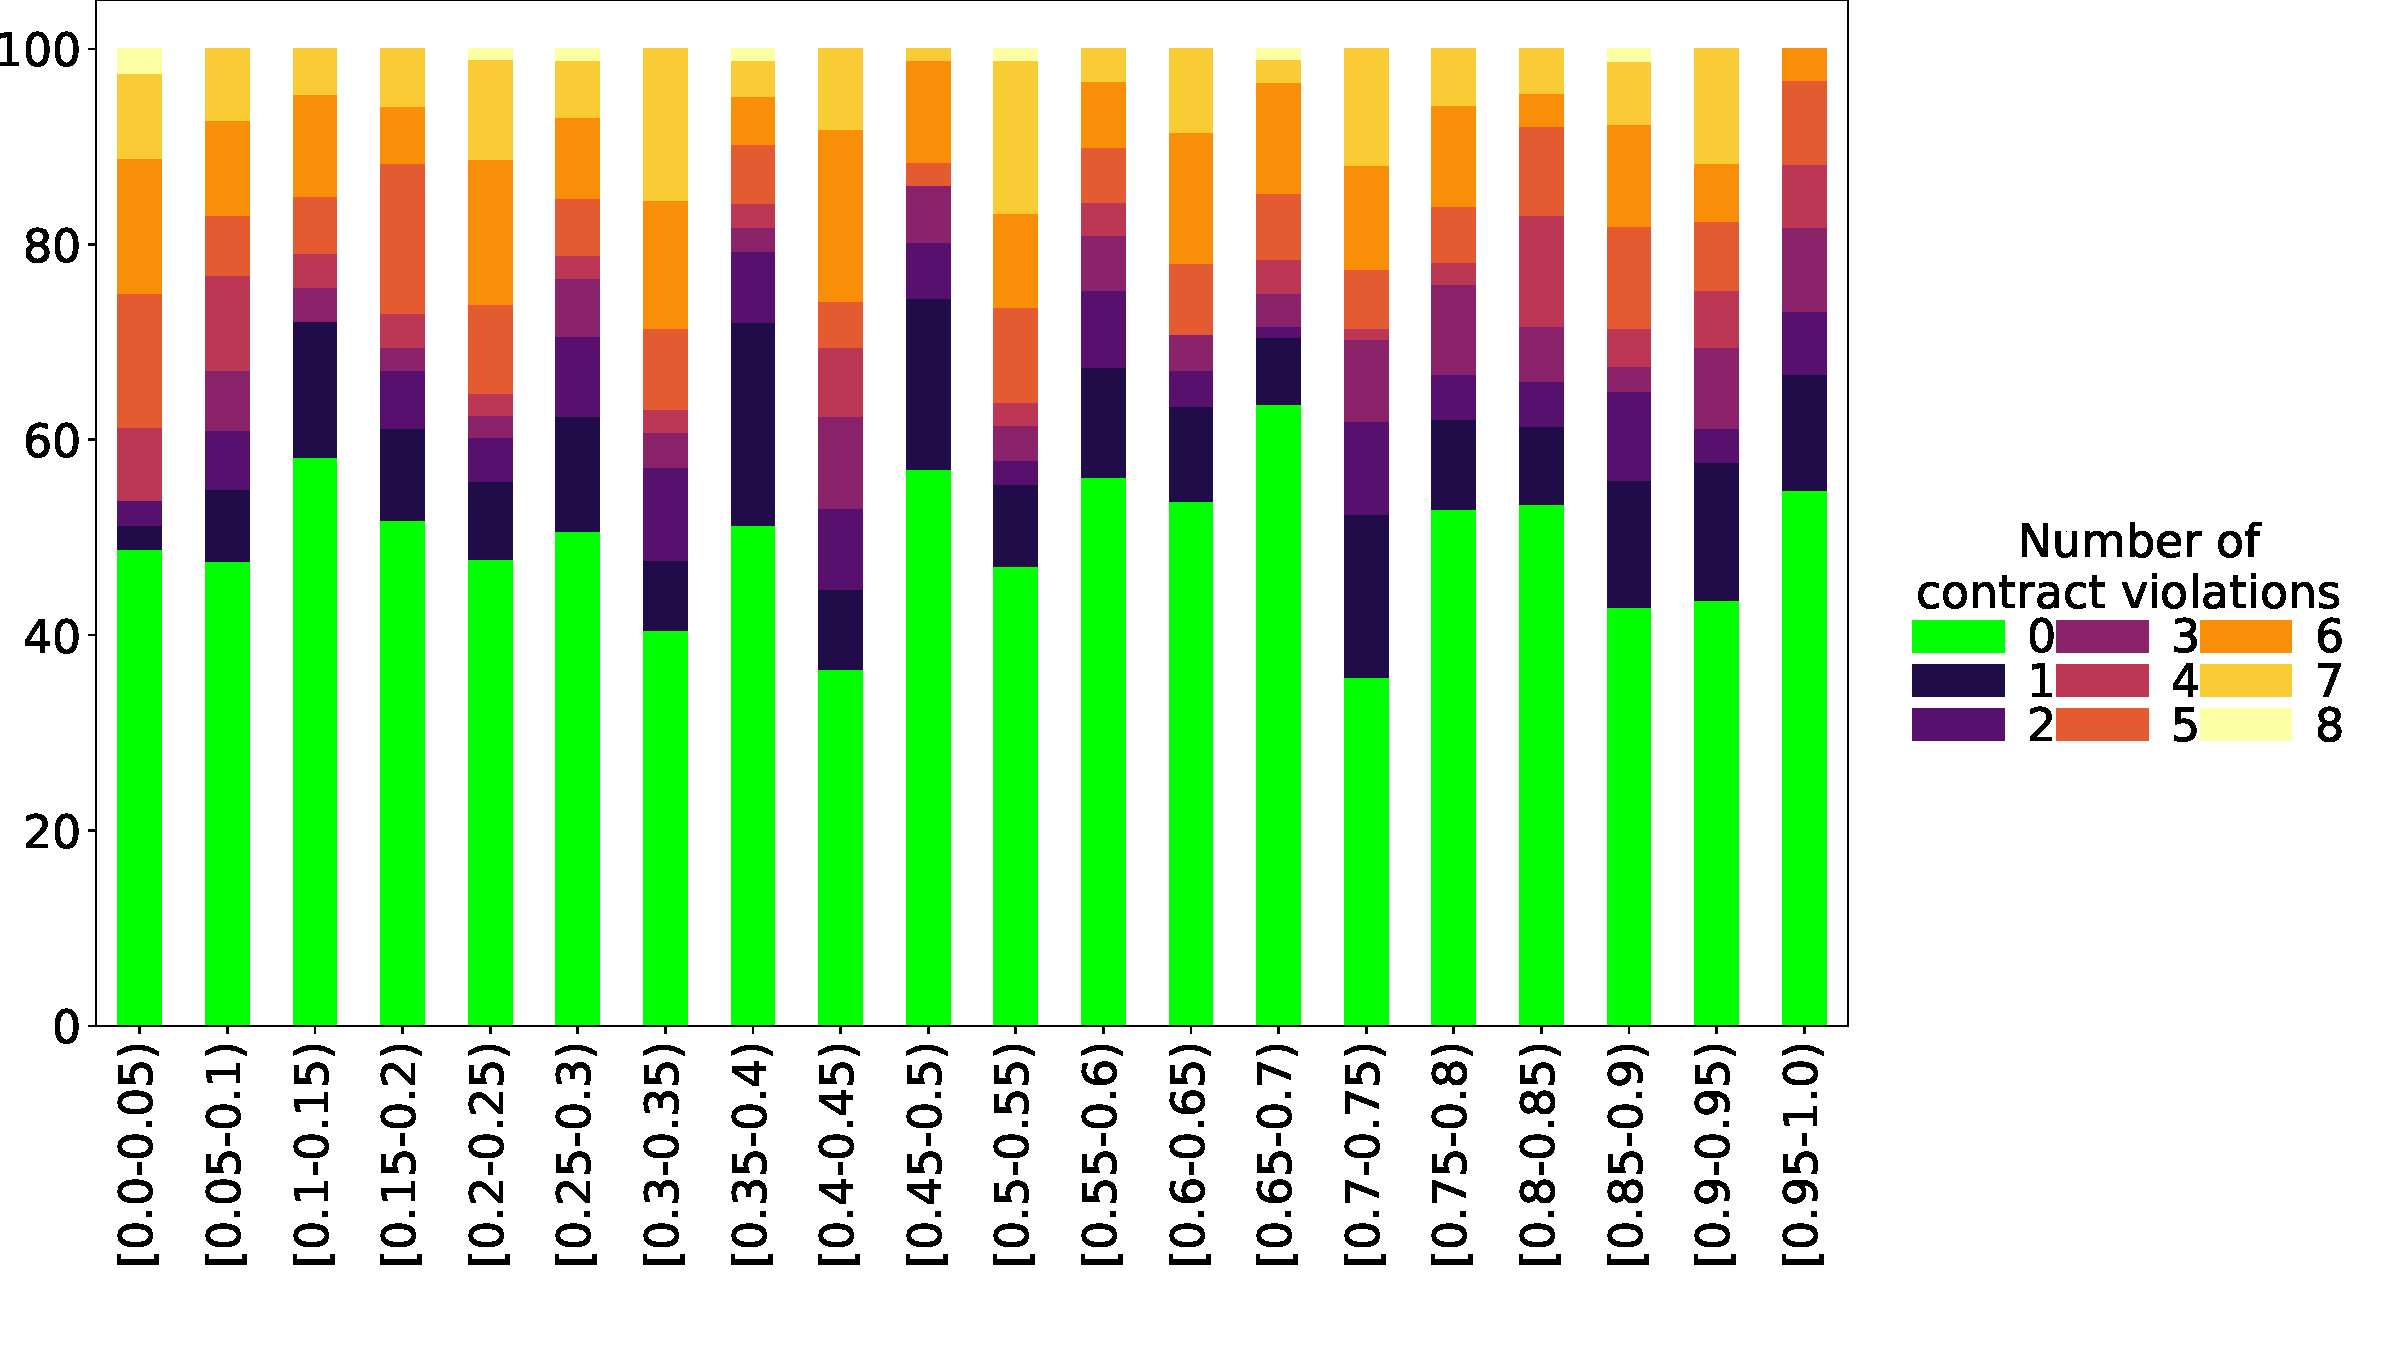
\includegraphics[width=\textwidth]{images/DistrValiditySmall/crossoverRate.pdf}
	\caption[crossoverRate parameter values distribution for smaller problem]{crossoverRate parameter values distribution for smaller problem}
	\label{fig:crossoverRate_DistSmall}
\end{figure}
\begin{figure}
	\centering
	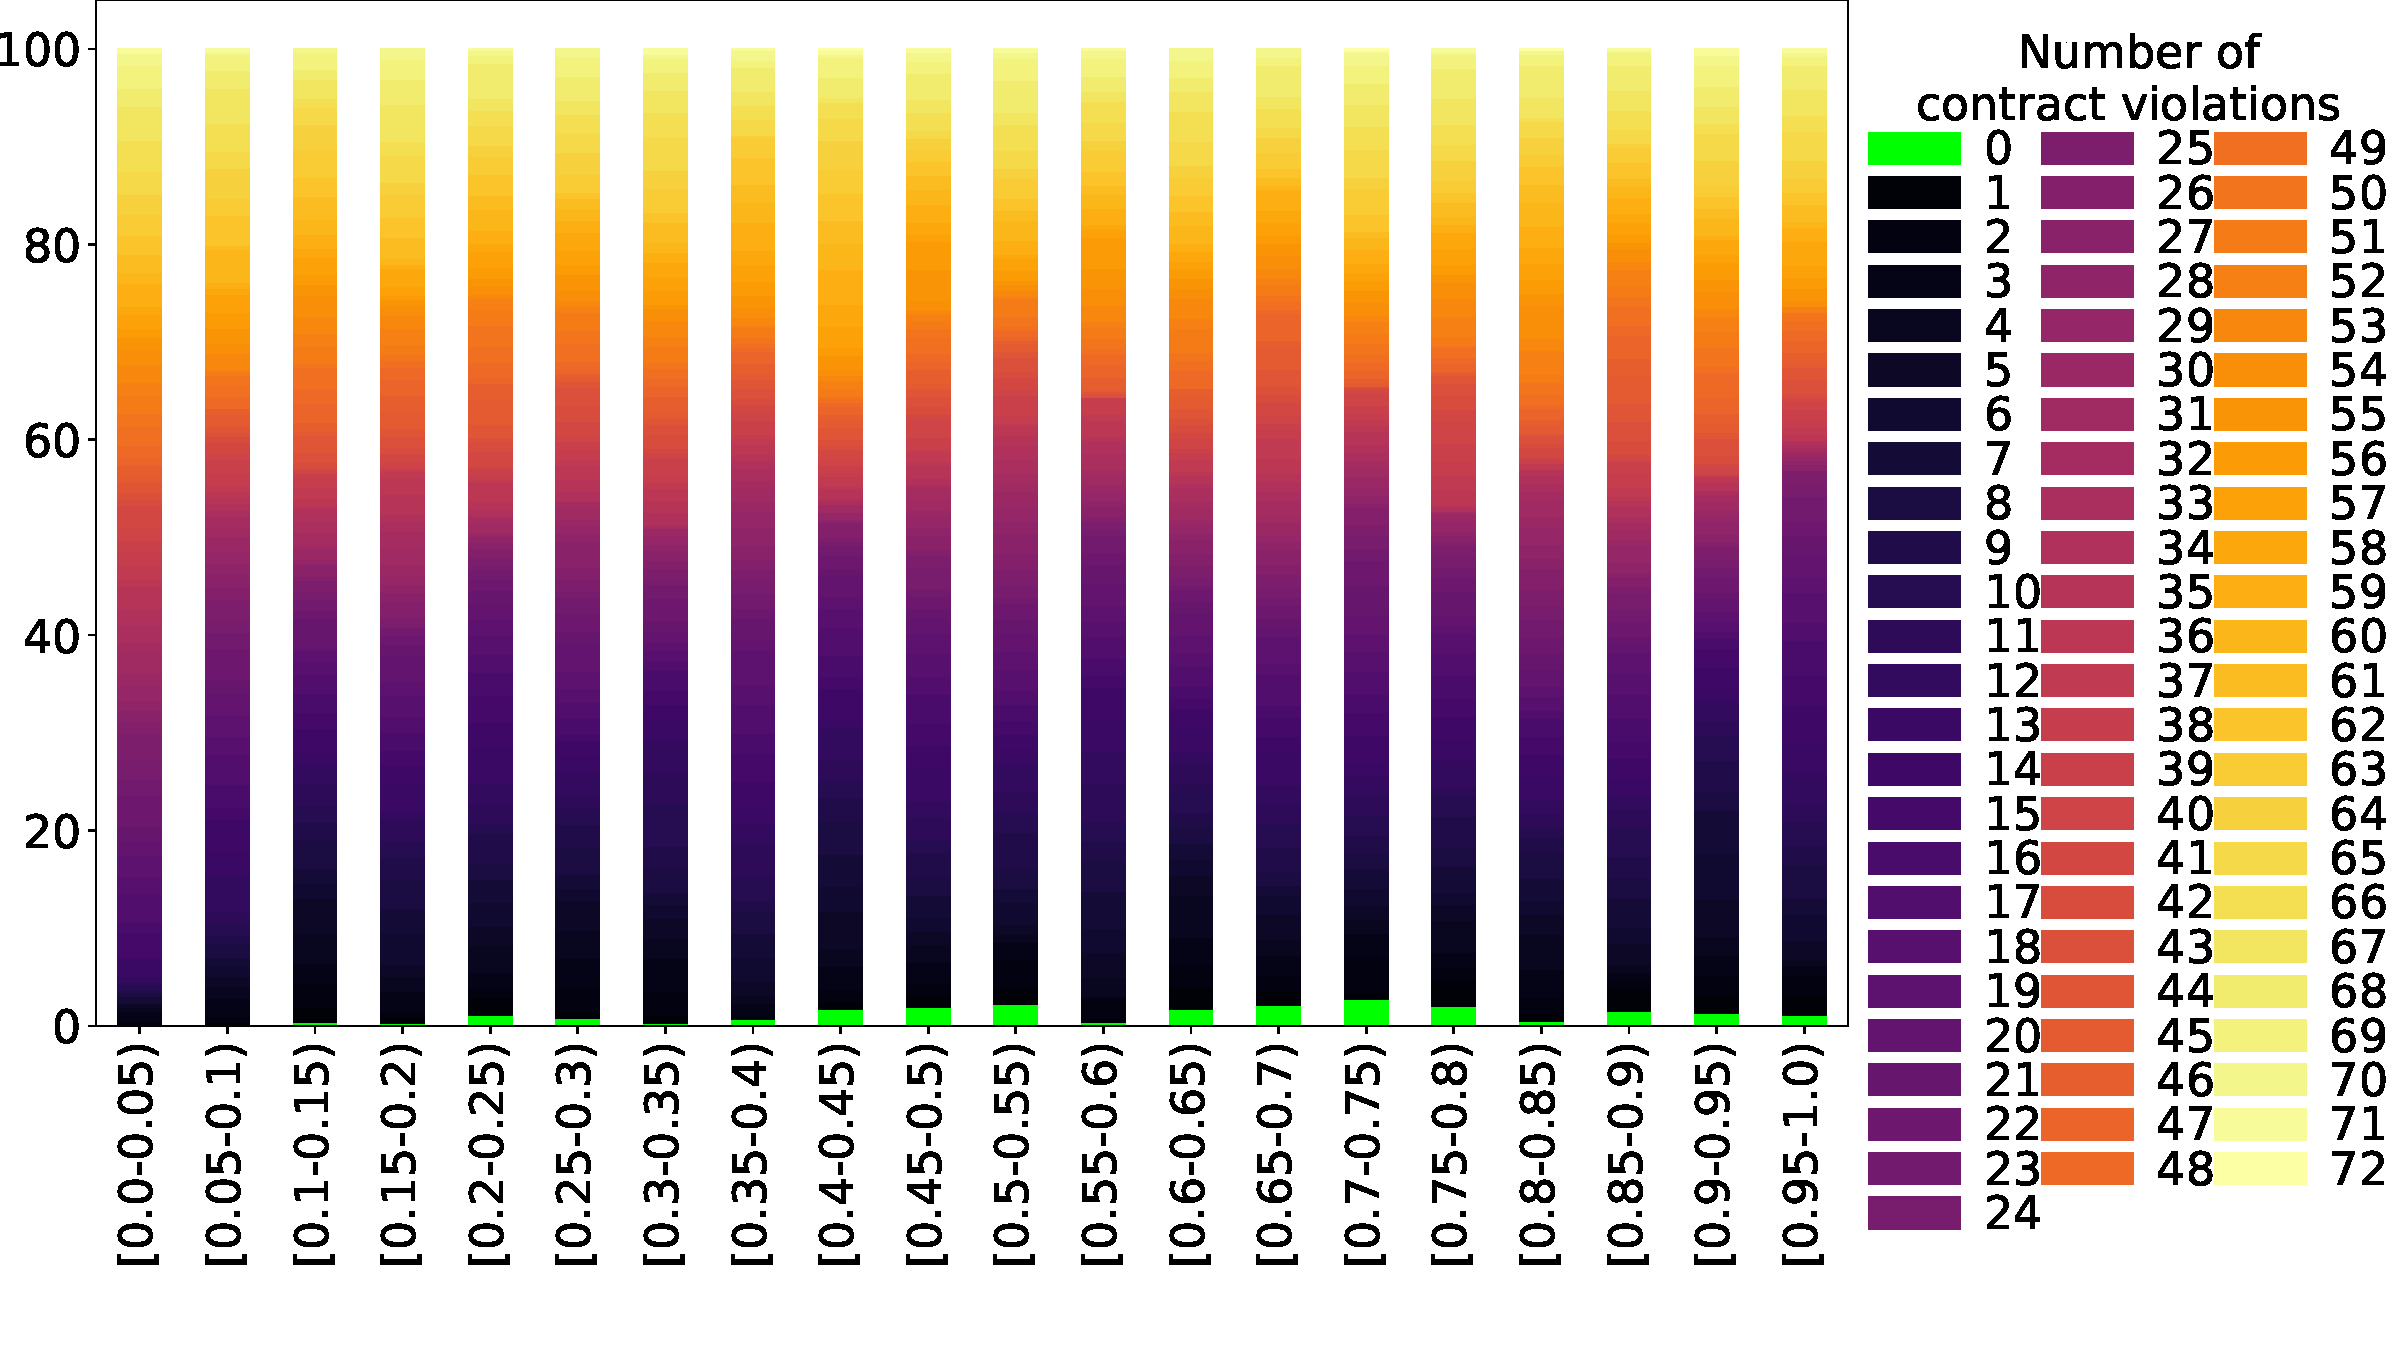
\includegraphics[width=\textwidth]{images/DistrValidityBig/mu.pdf}
	\caption[mu parameter values distribution for bigger problem]{mu parameter values distribution for bigger problem}
	\label{fig:mu_DistBig}
\end{figure}
\begin{figure}
	\centering
	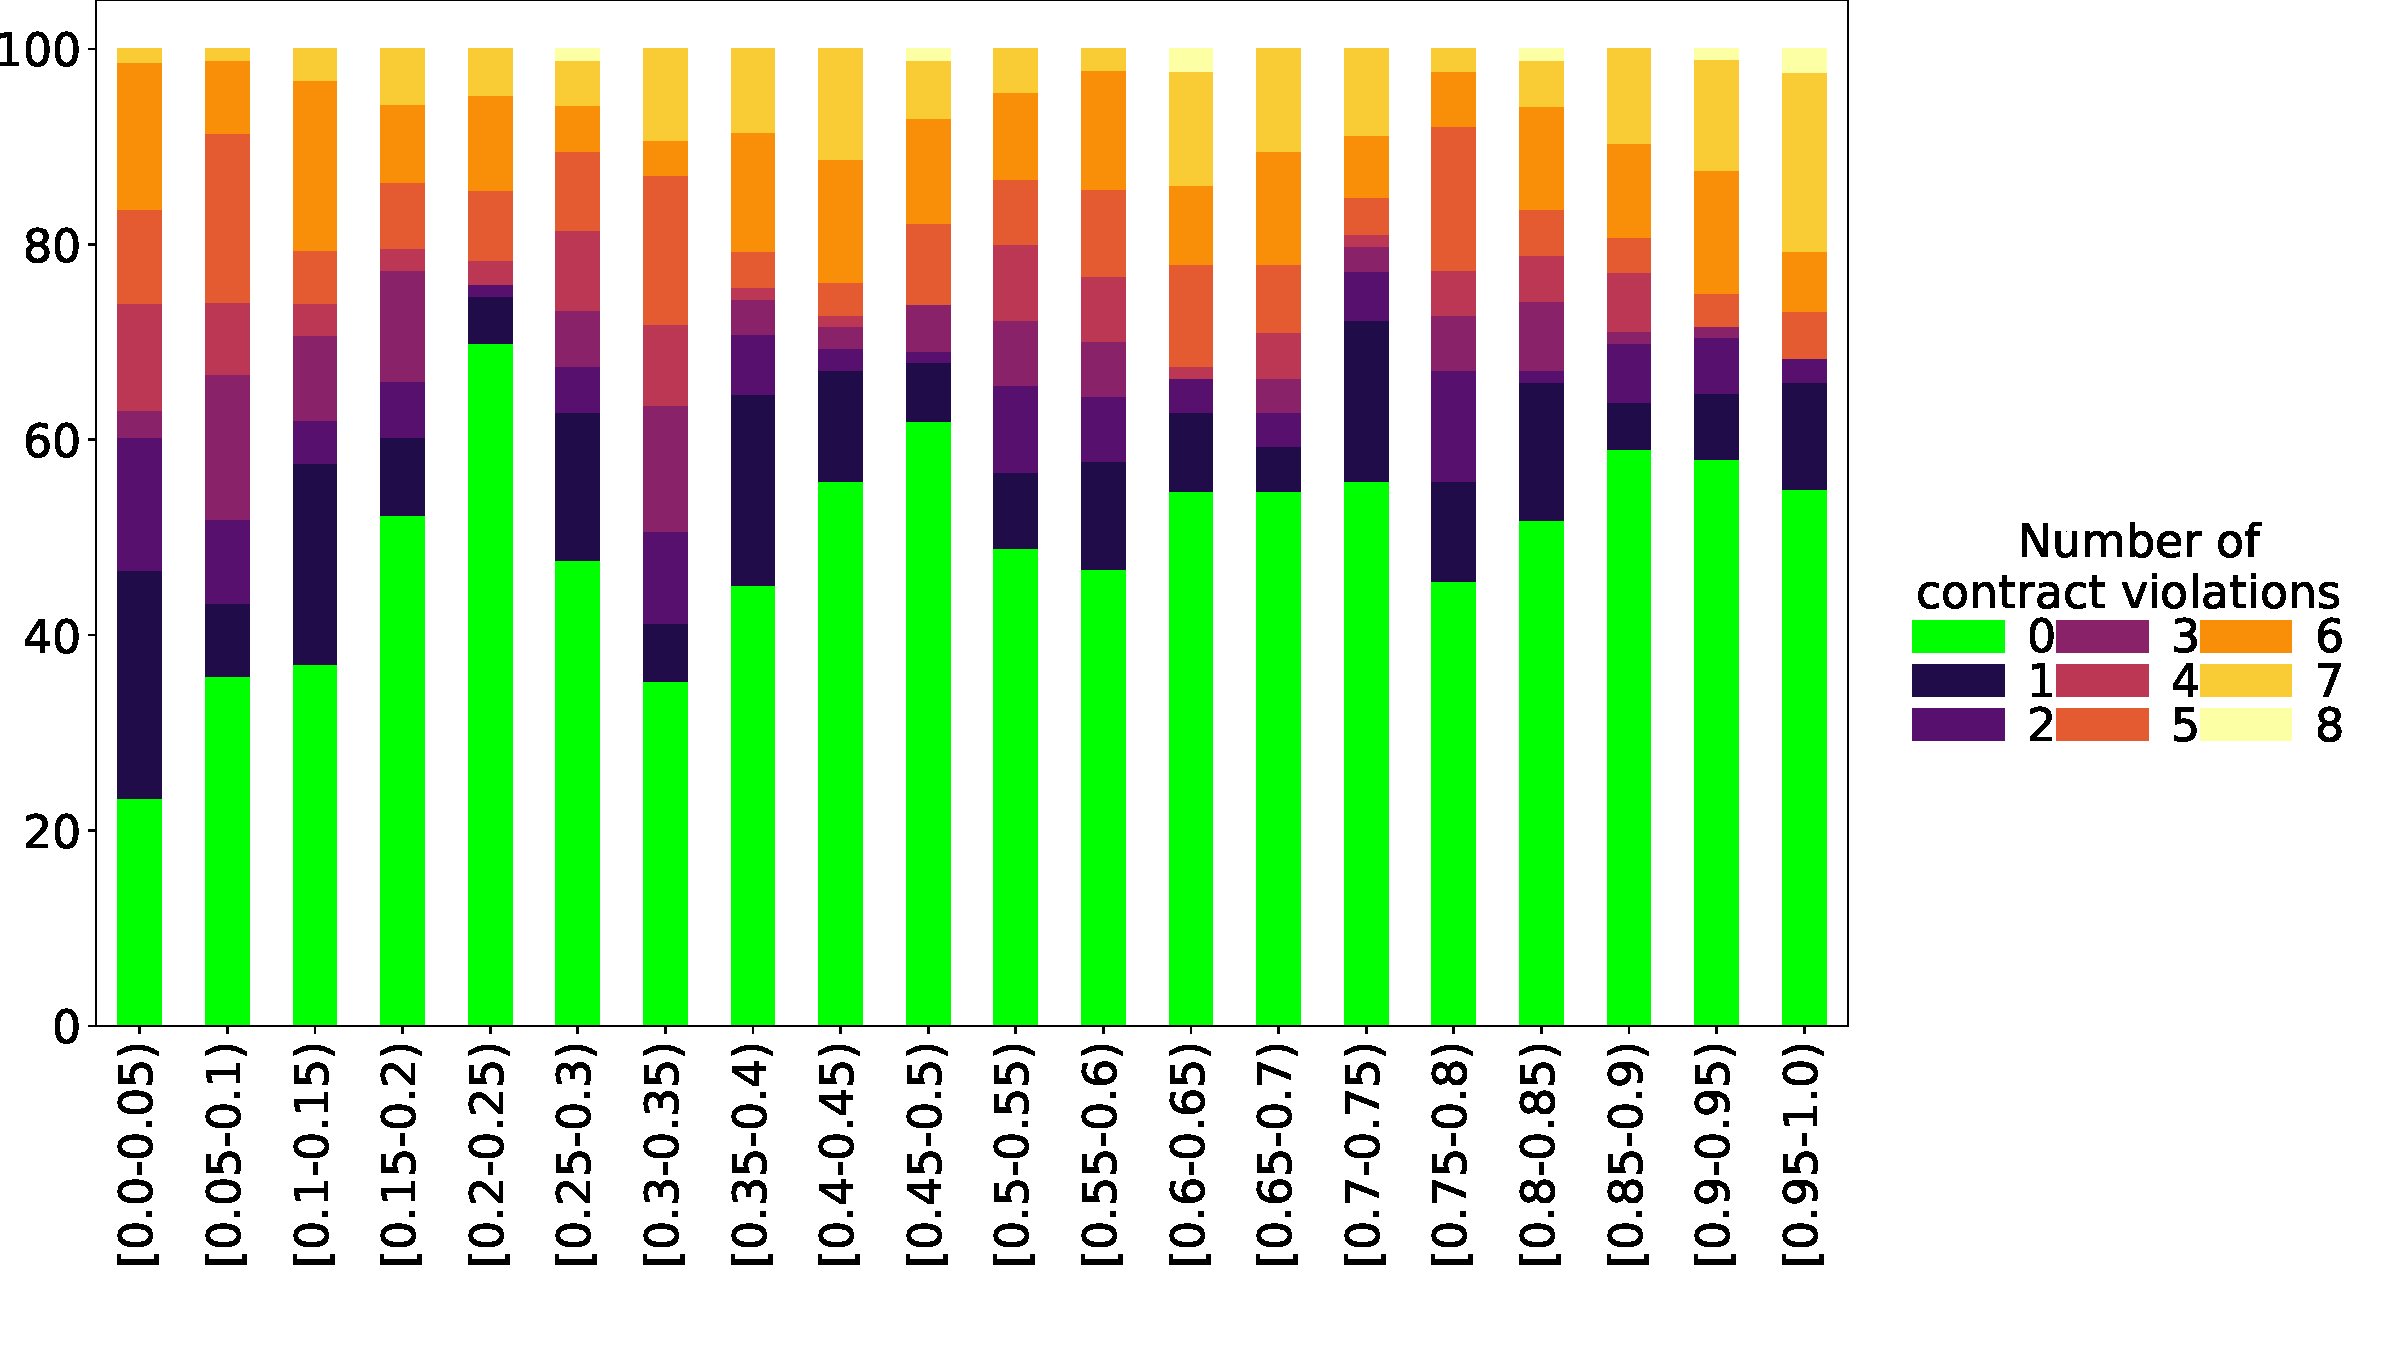
\includegraphics[width=\textwidth]{images/DistrValiditySmall/mu.pdf}
	\caption[mu parameter values distribution for smaller problem]{mu parameter values distribution for smaller problem}
	\label{fig:mu_DistSmall}
\end{figure}
\begin{figure}
	\centering
	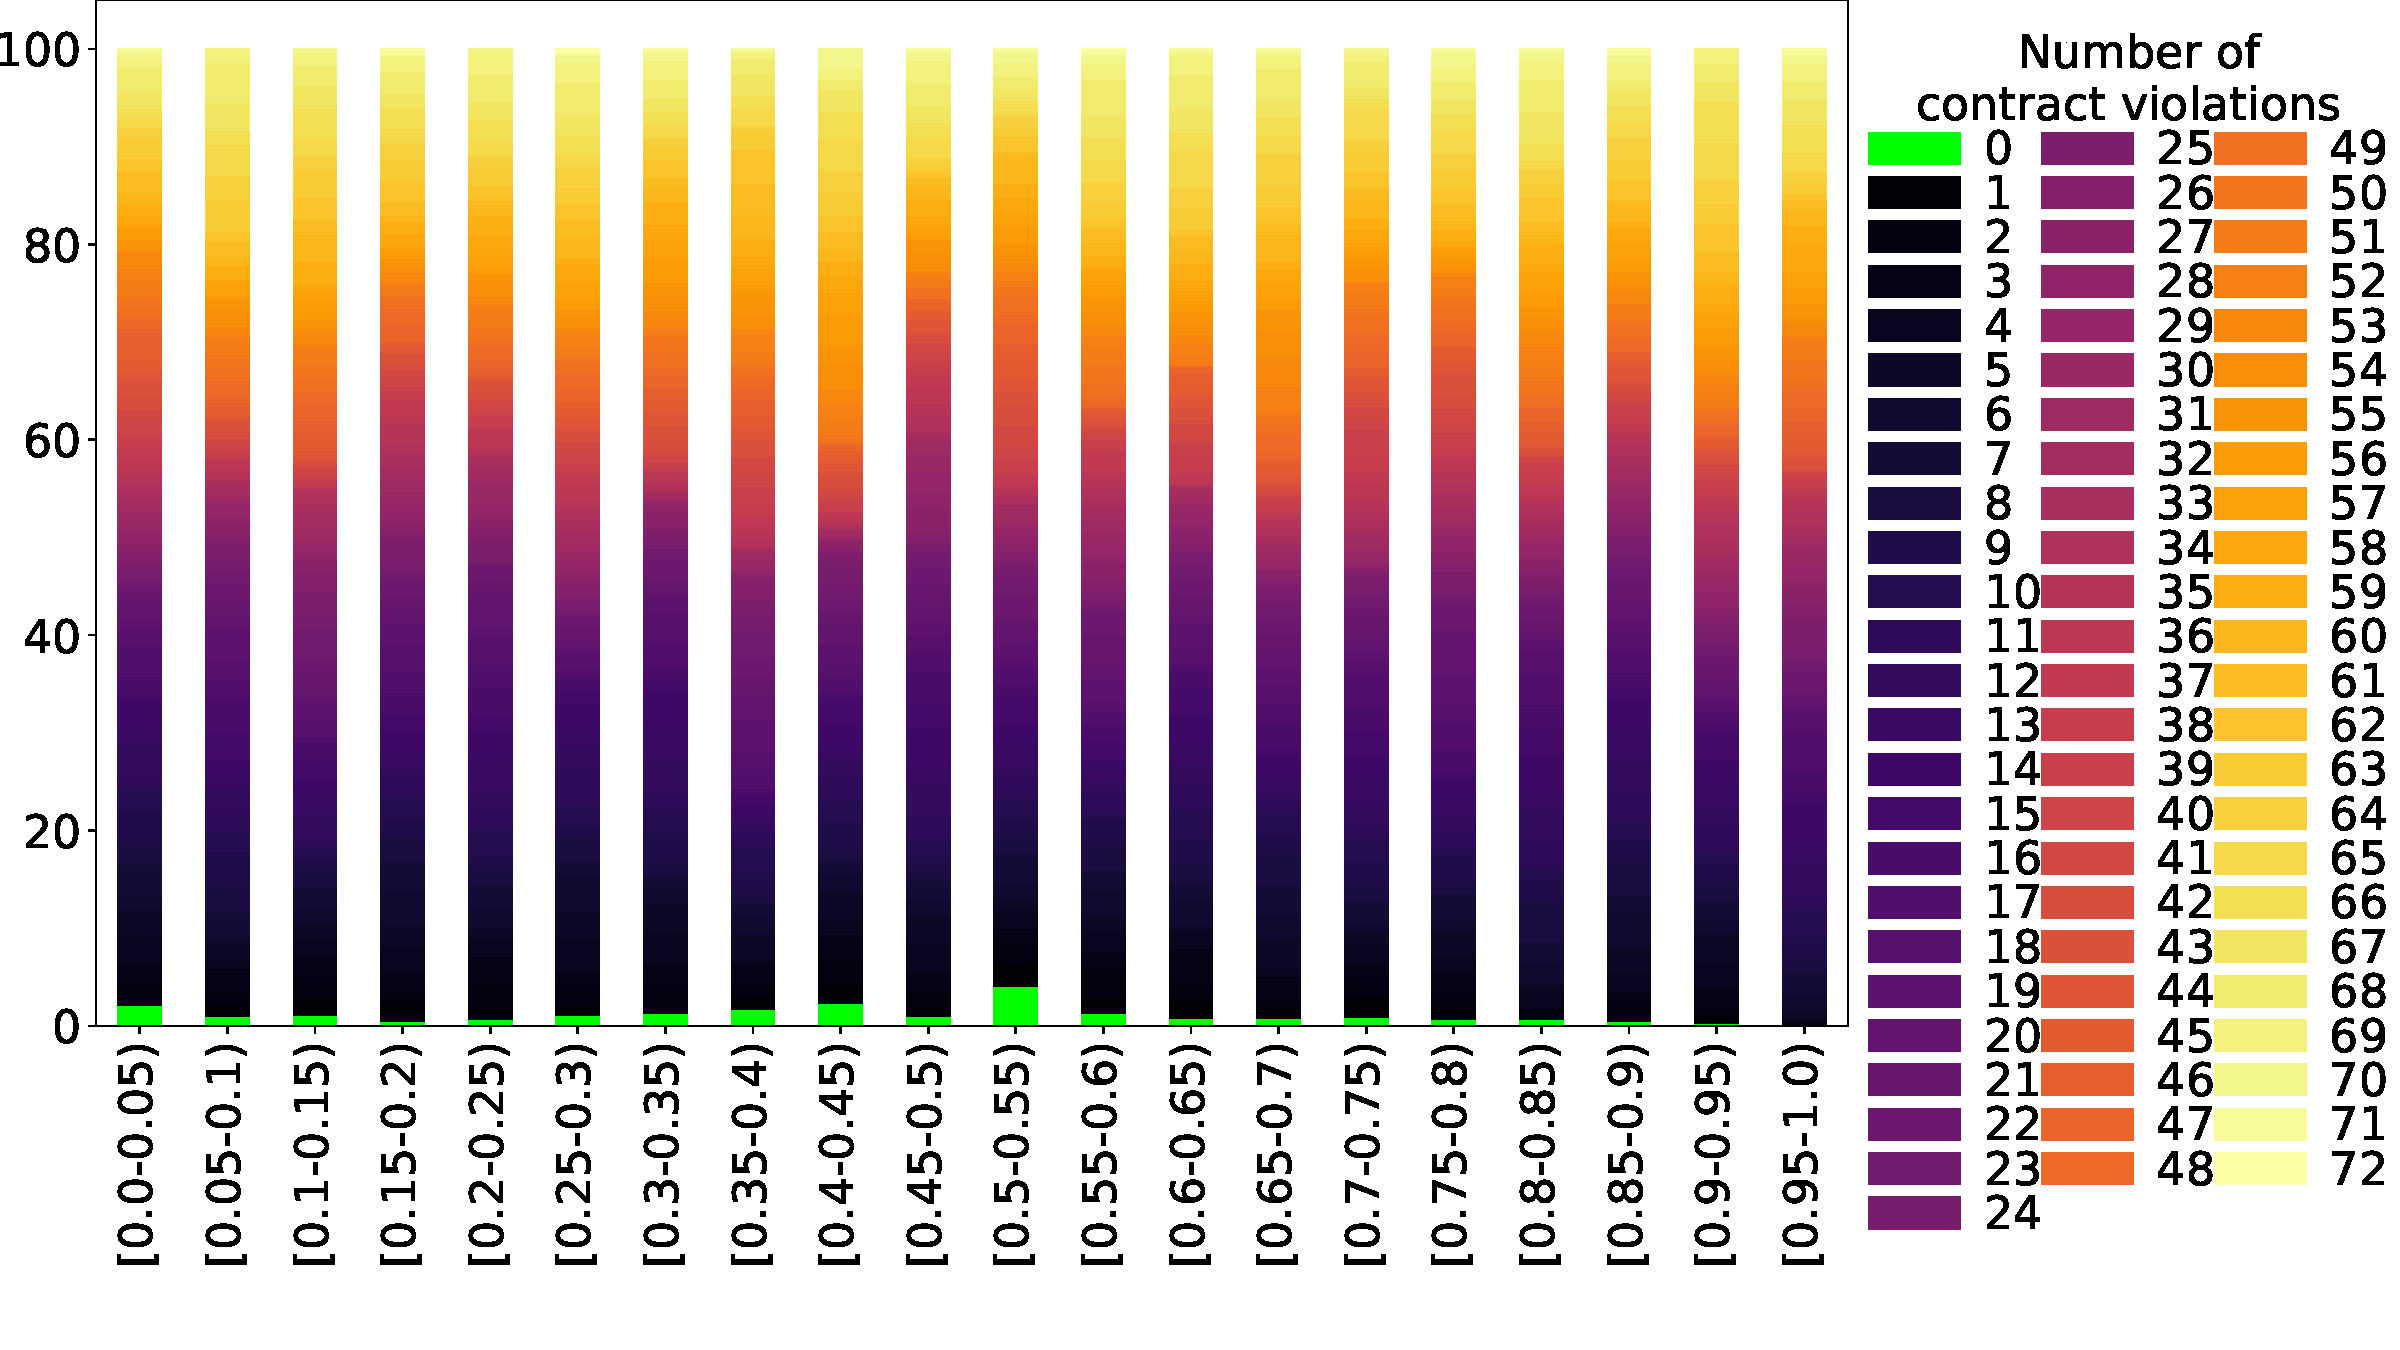
\includegraphics[width=\textwidth]{images/DistrValidityBig/mutationRate.pdf}
	\caption[mutationRate parameter values distribution for bigger problem]{mutationRate parameter values distribution for bigger problem}
	\label{fig:mutationRate_DistBig}
\end{figure}
\begin{figure}
	\centering
	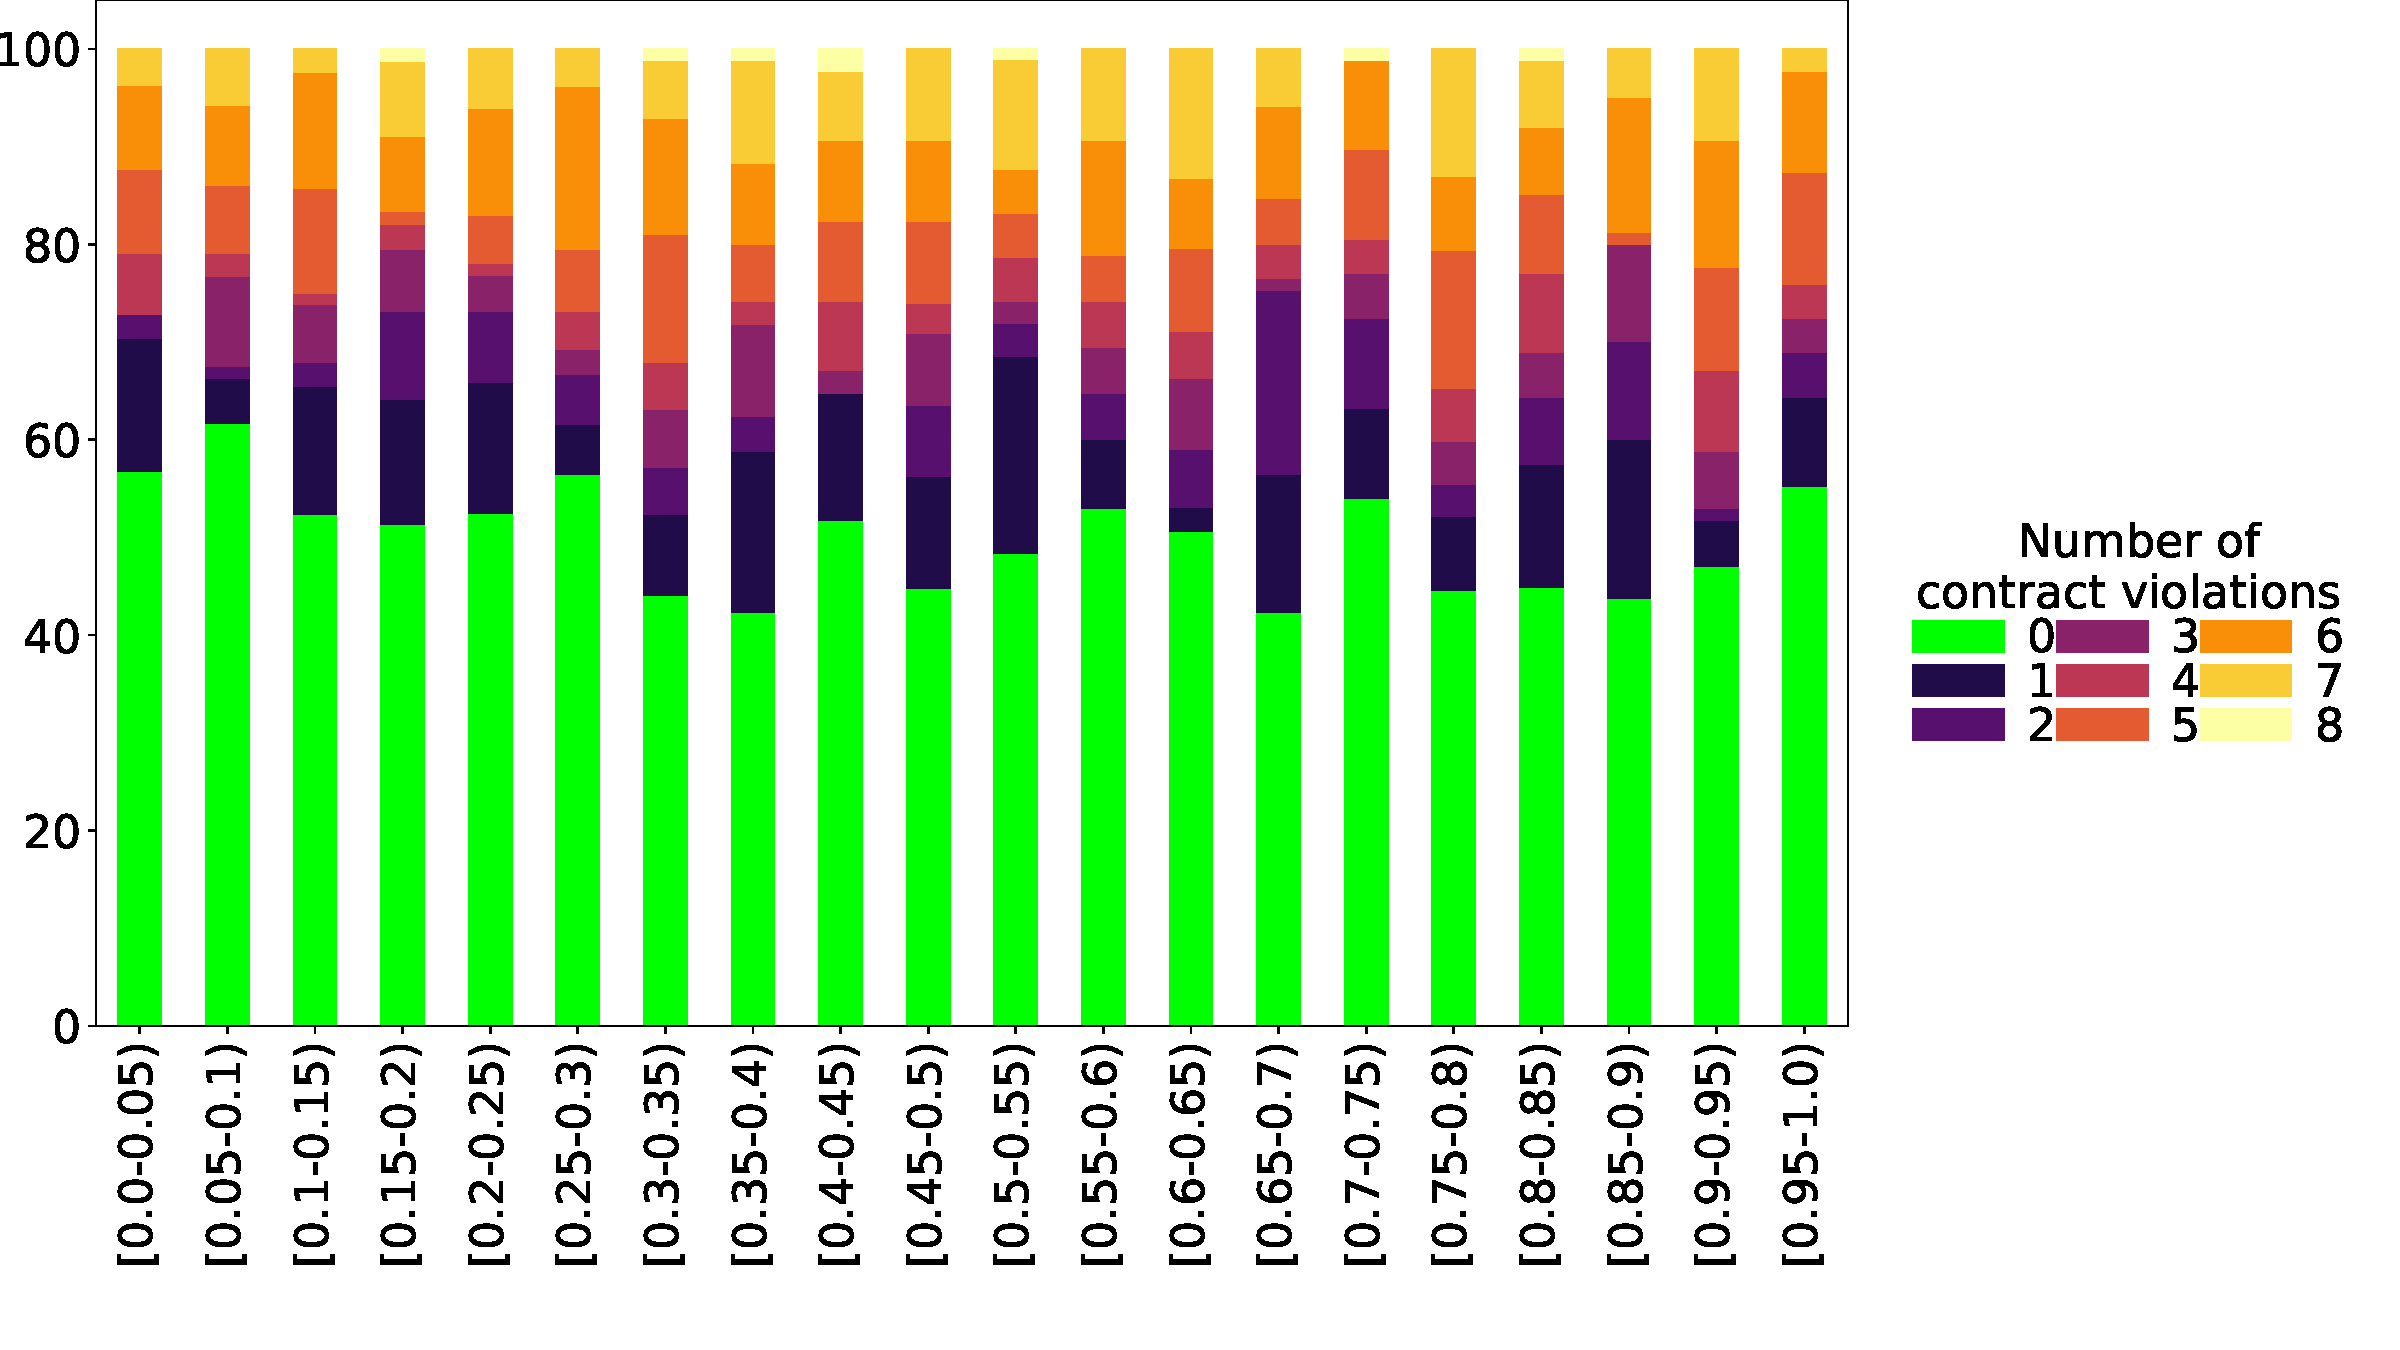
\includegraphics[width=\textwidth]{images/DistrValiditySmall/mutationRate.pdf}
	\caption[mutationRate parameter values distribution for smaller problem]{mutationRate parameter values distribution for smaller problem}
	\label{fig:mutationRate_DistSmall}
\end{figure}
\begin{figure}
	\centering
	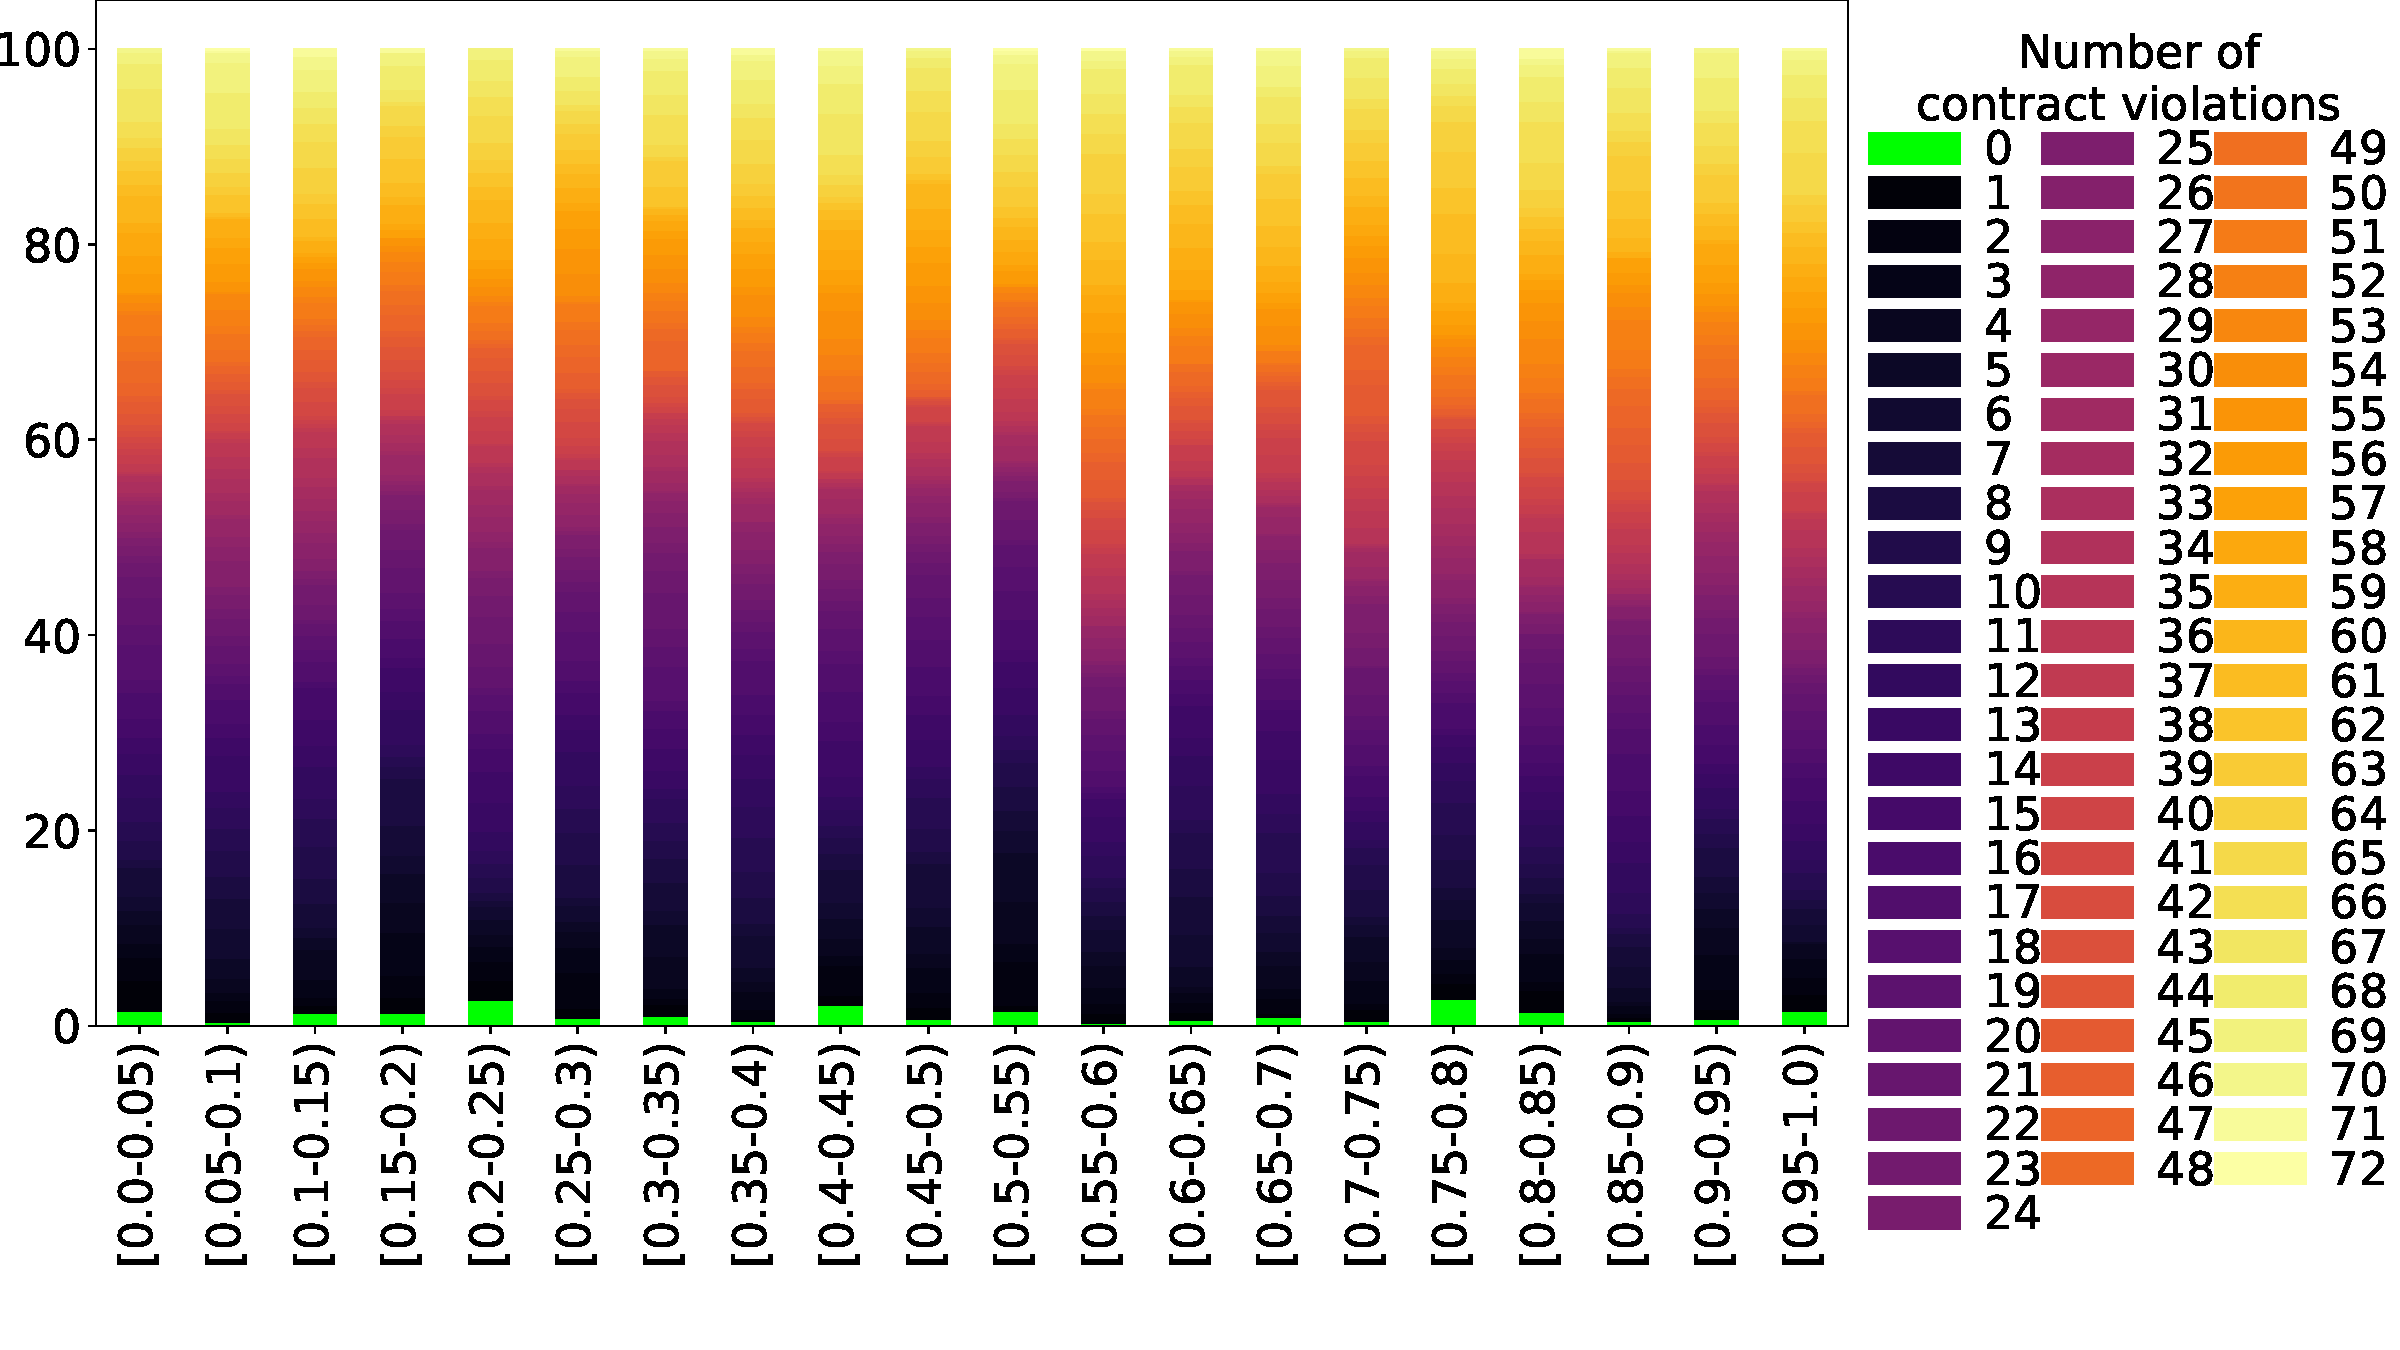
\includegraphics[width=\textwidth]{images/DistrValidityBig/resourcesMutationProbability.pdf}
	\caption[resourcesMutationProbability parameter values distribution for bigger problem]{resourcesMutationProbability parameter values distribution for bigger problem}
	\label{fig:resourcesMutationProbability_DistBig}
\end{figure}
\begin{figure}
	\centering
	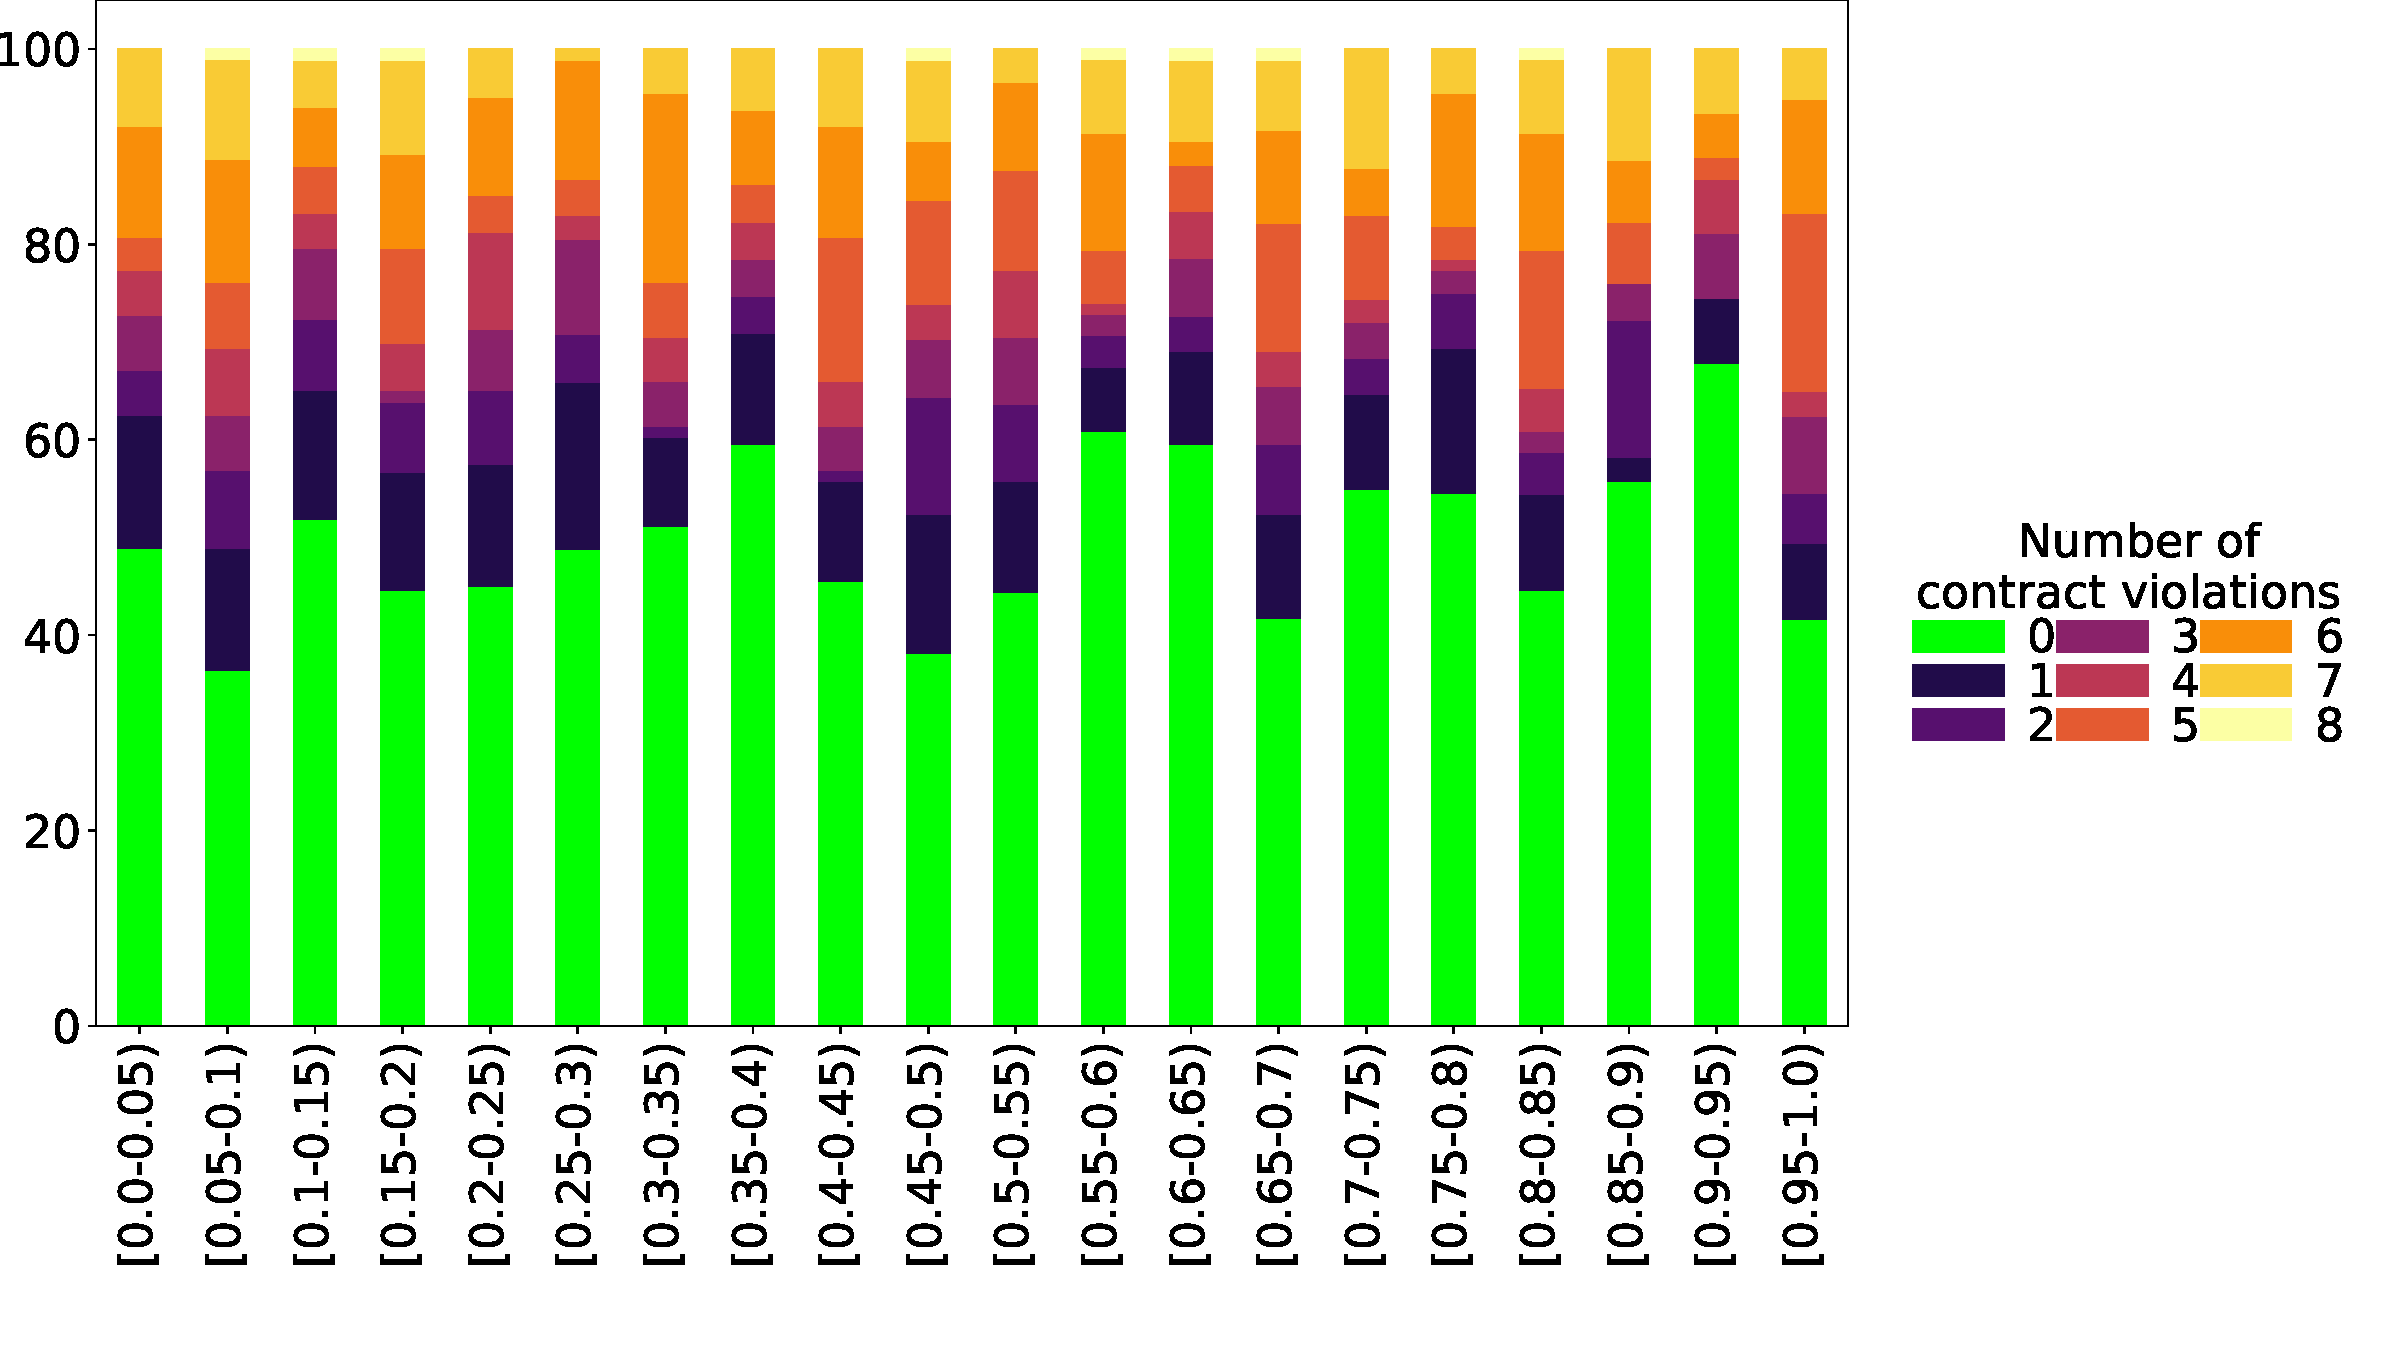
\includegraphics[width=\textwidth]{images/DistrValiditySmall/resourcesMutationProbability.pdf}
	\caption[resourcesMutationProbability parameter values distribution for smaller problem]{resourcesMutationProbability parameter values distribution for smaller problem}
	\label{fig:resourcesMutationProbability_DistSmall}
\end{figure}
\begin{figure}
	\centering
	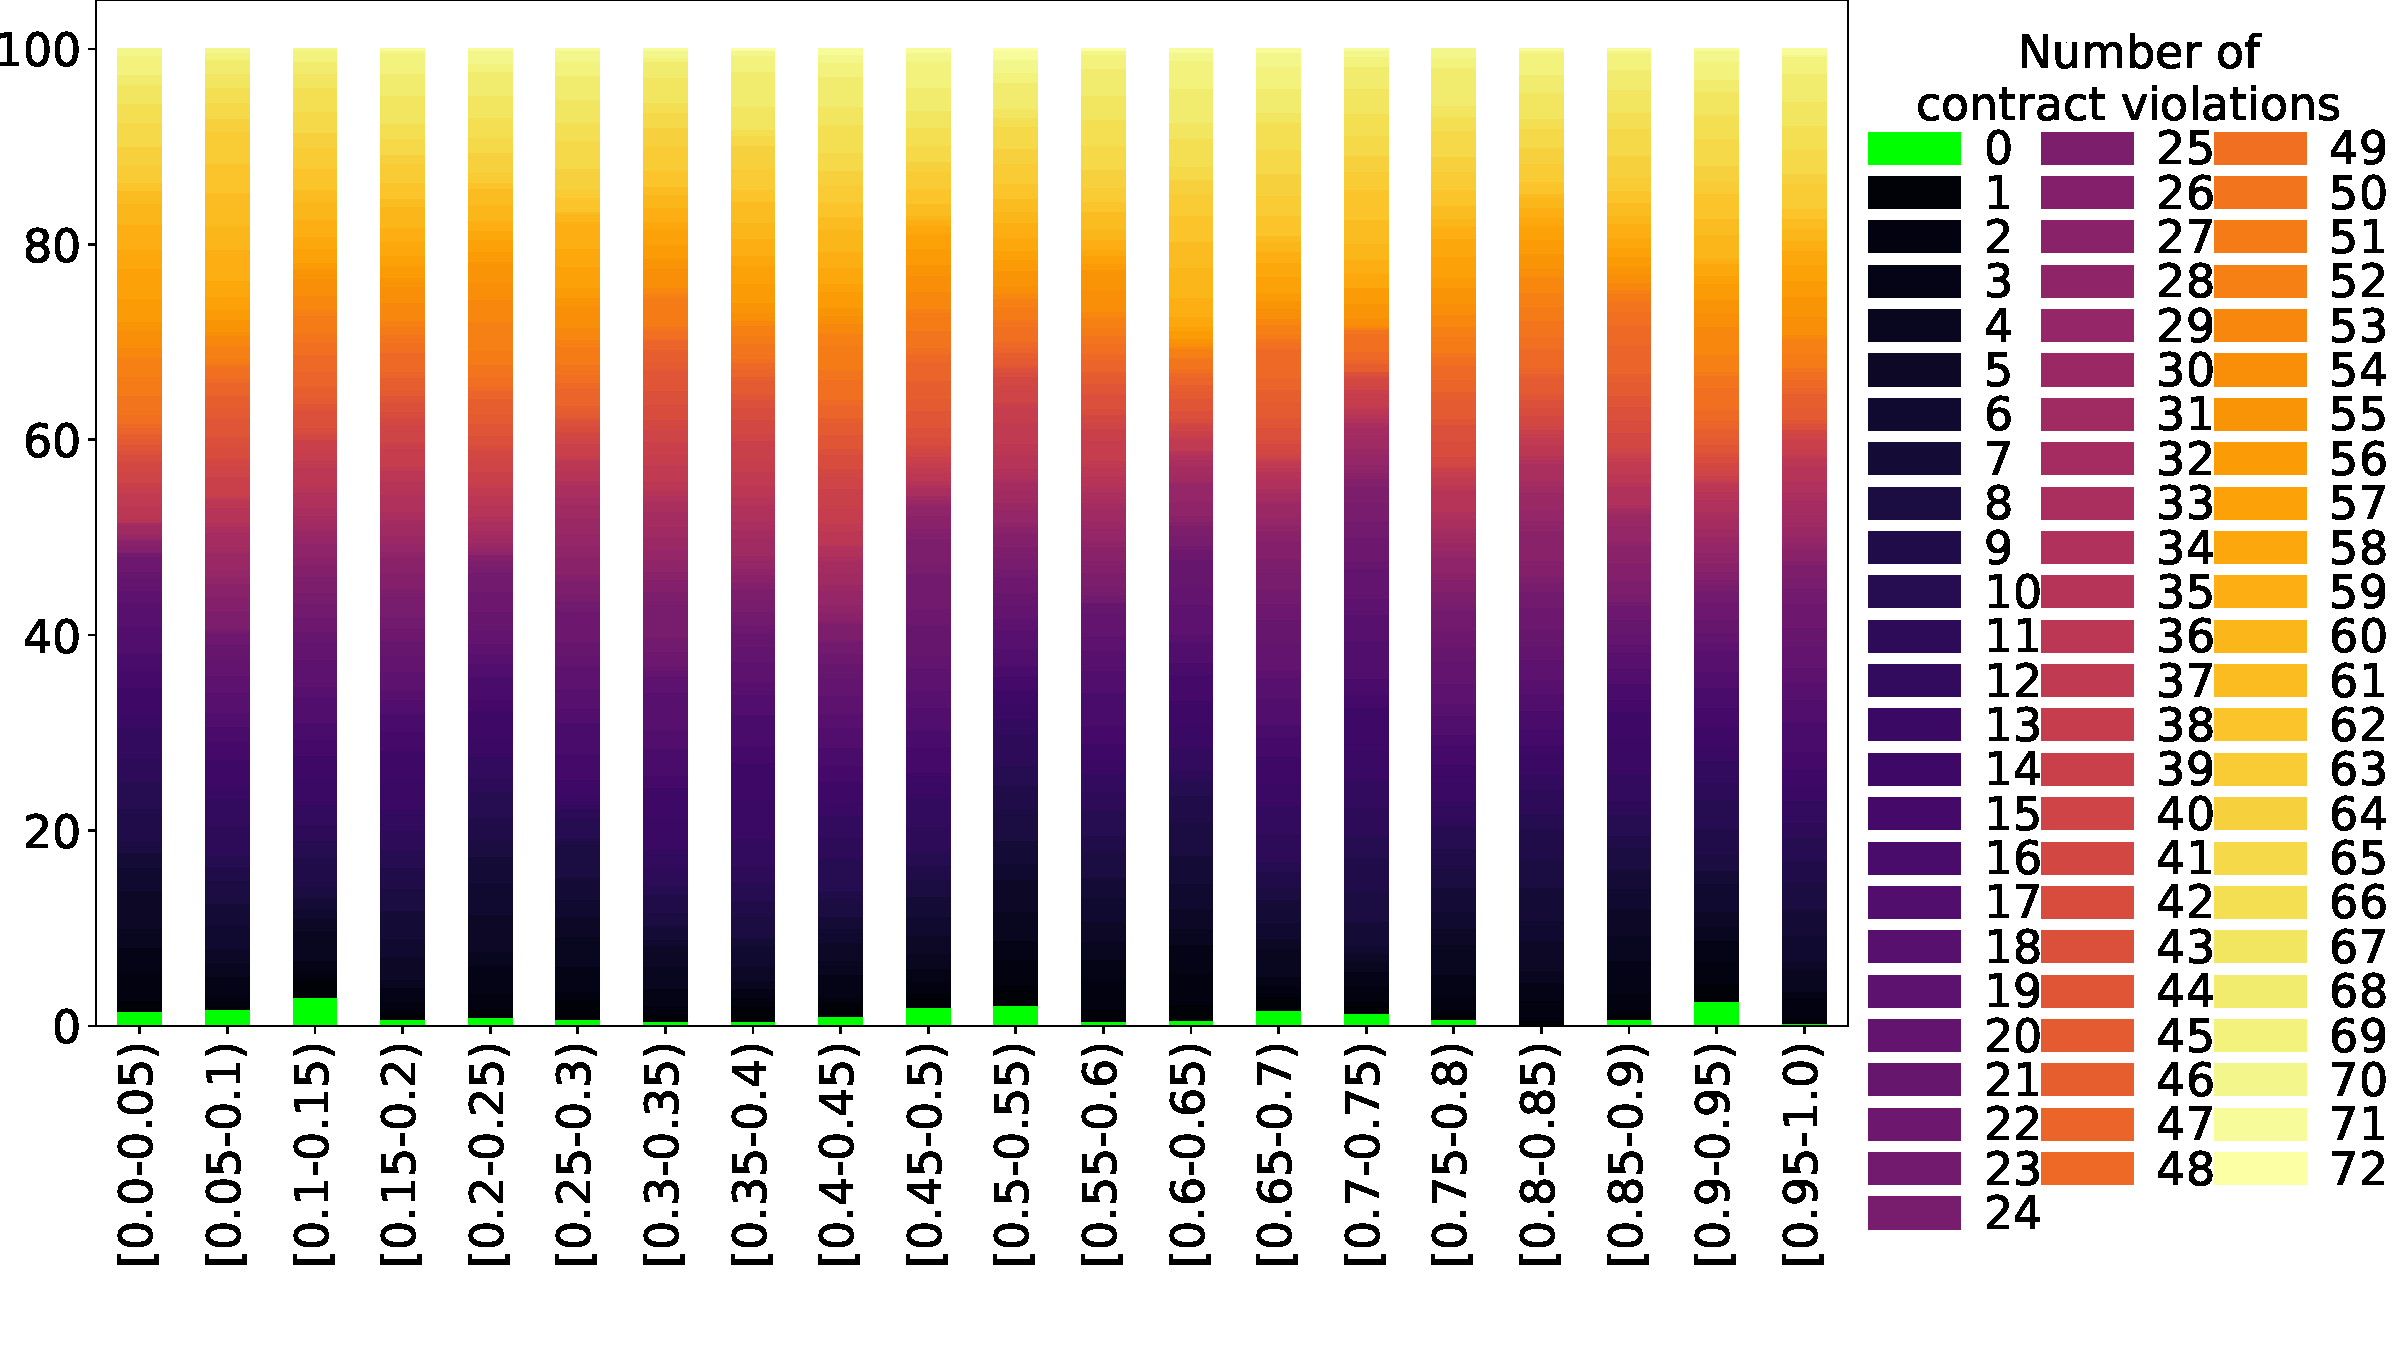
\includegraphics[width=\textwidth]{images/DistrValidityBig/crossoverOnRandomChildProbability.pdf}
	\caption[crossoverOnRandomChildProbability parameter values distribution for bigger problem]{crossoverOnRandomChildProbability parameter values distribution for bigger problem}
	\label{fig:crossoverOnRandomChildProbability_DistBig}
\end{figure}
\begin{figure}
	\centering
	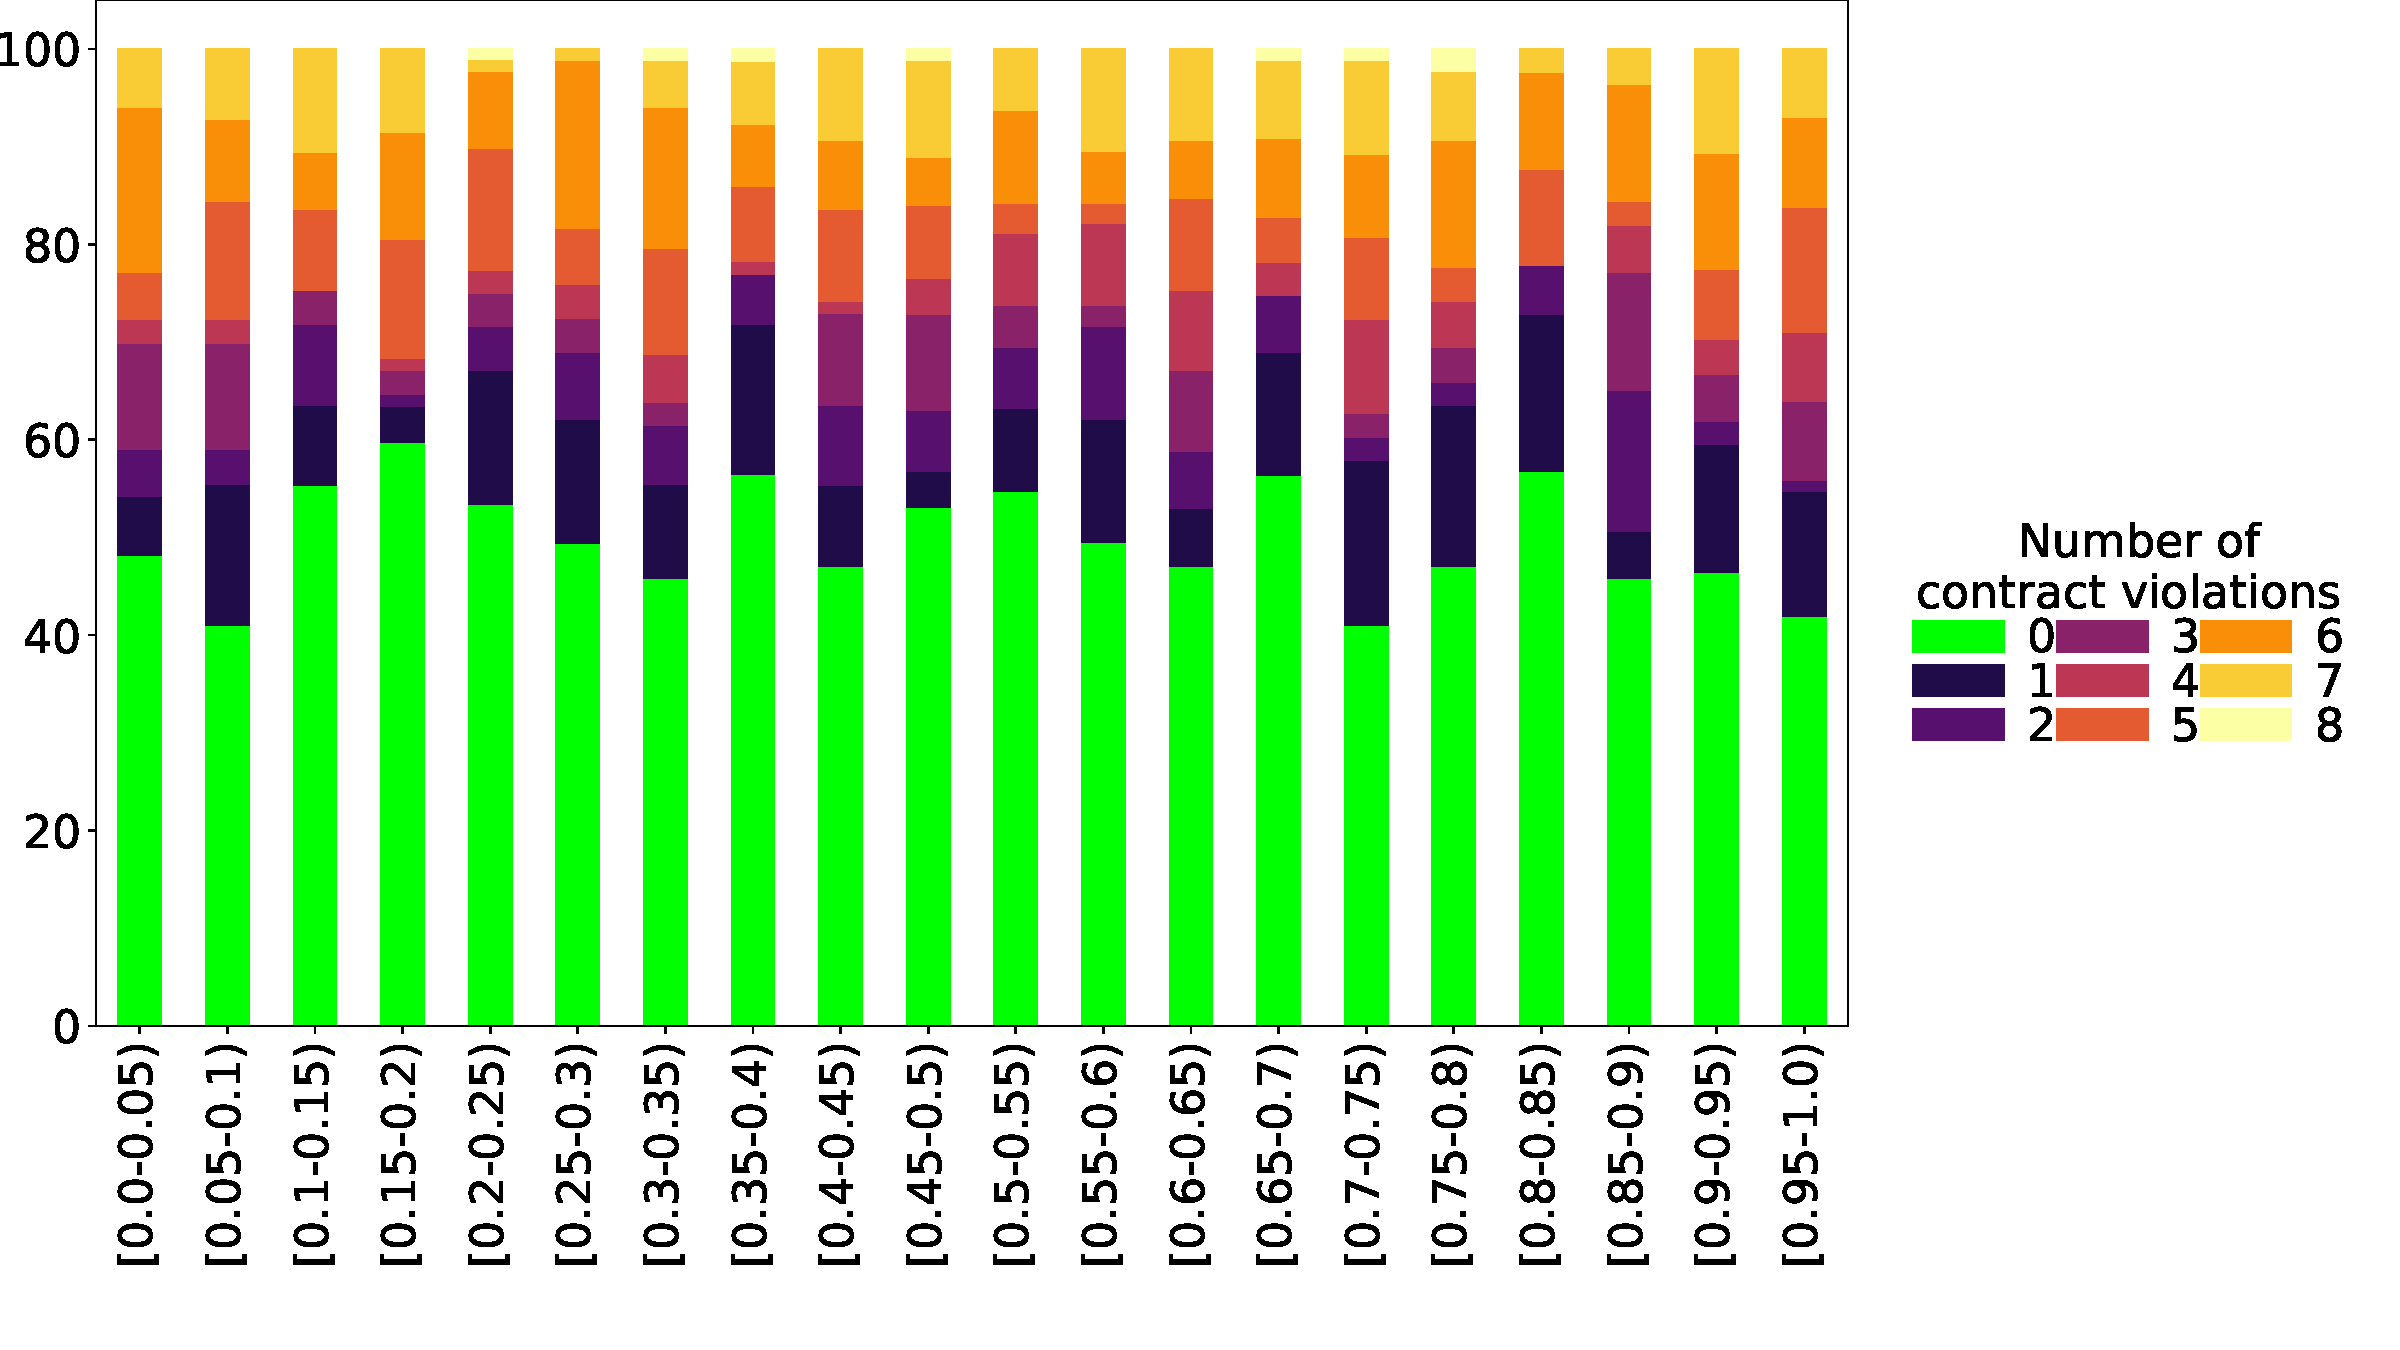
\includegraphics[width=\textwidth]{images/DistrValiditySmall/crossoverOnRandomChildProbability.pdf}
	\caption[crossoverOnRandomChildProbability parameter values distribution for smaller problem]{crossoverOnRandomChildProbability parameter values distribution for smaller problem}
	\label{fig:crossoverOnRandomChildProbability_DistSmall}
\end{figure}
\begin{figure}
	\centering
	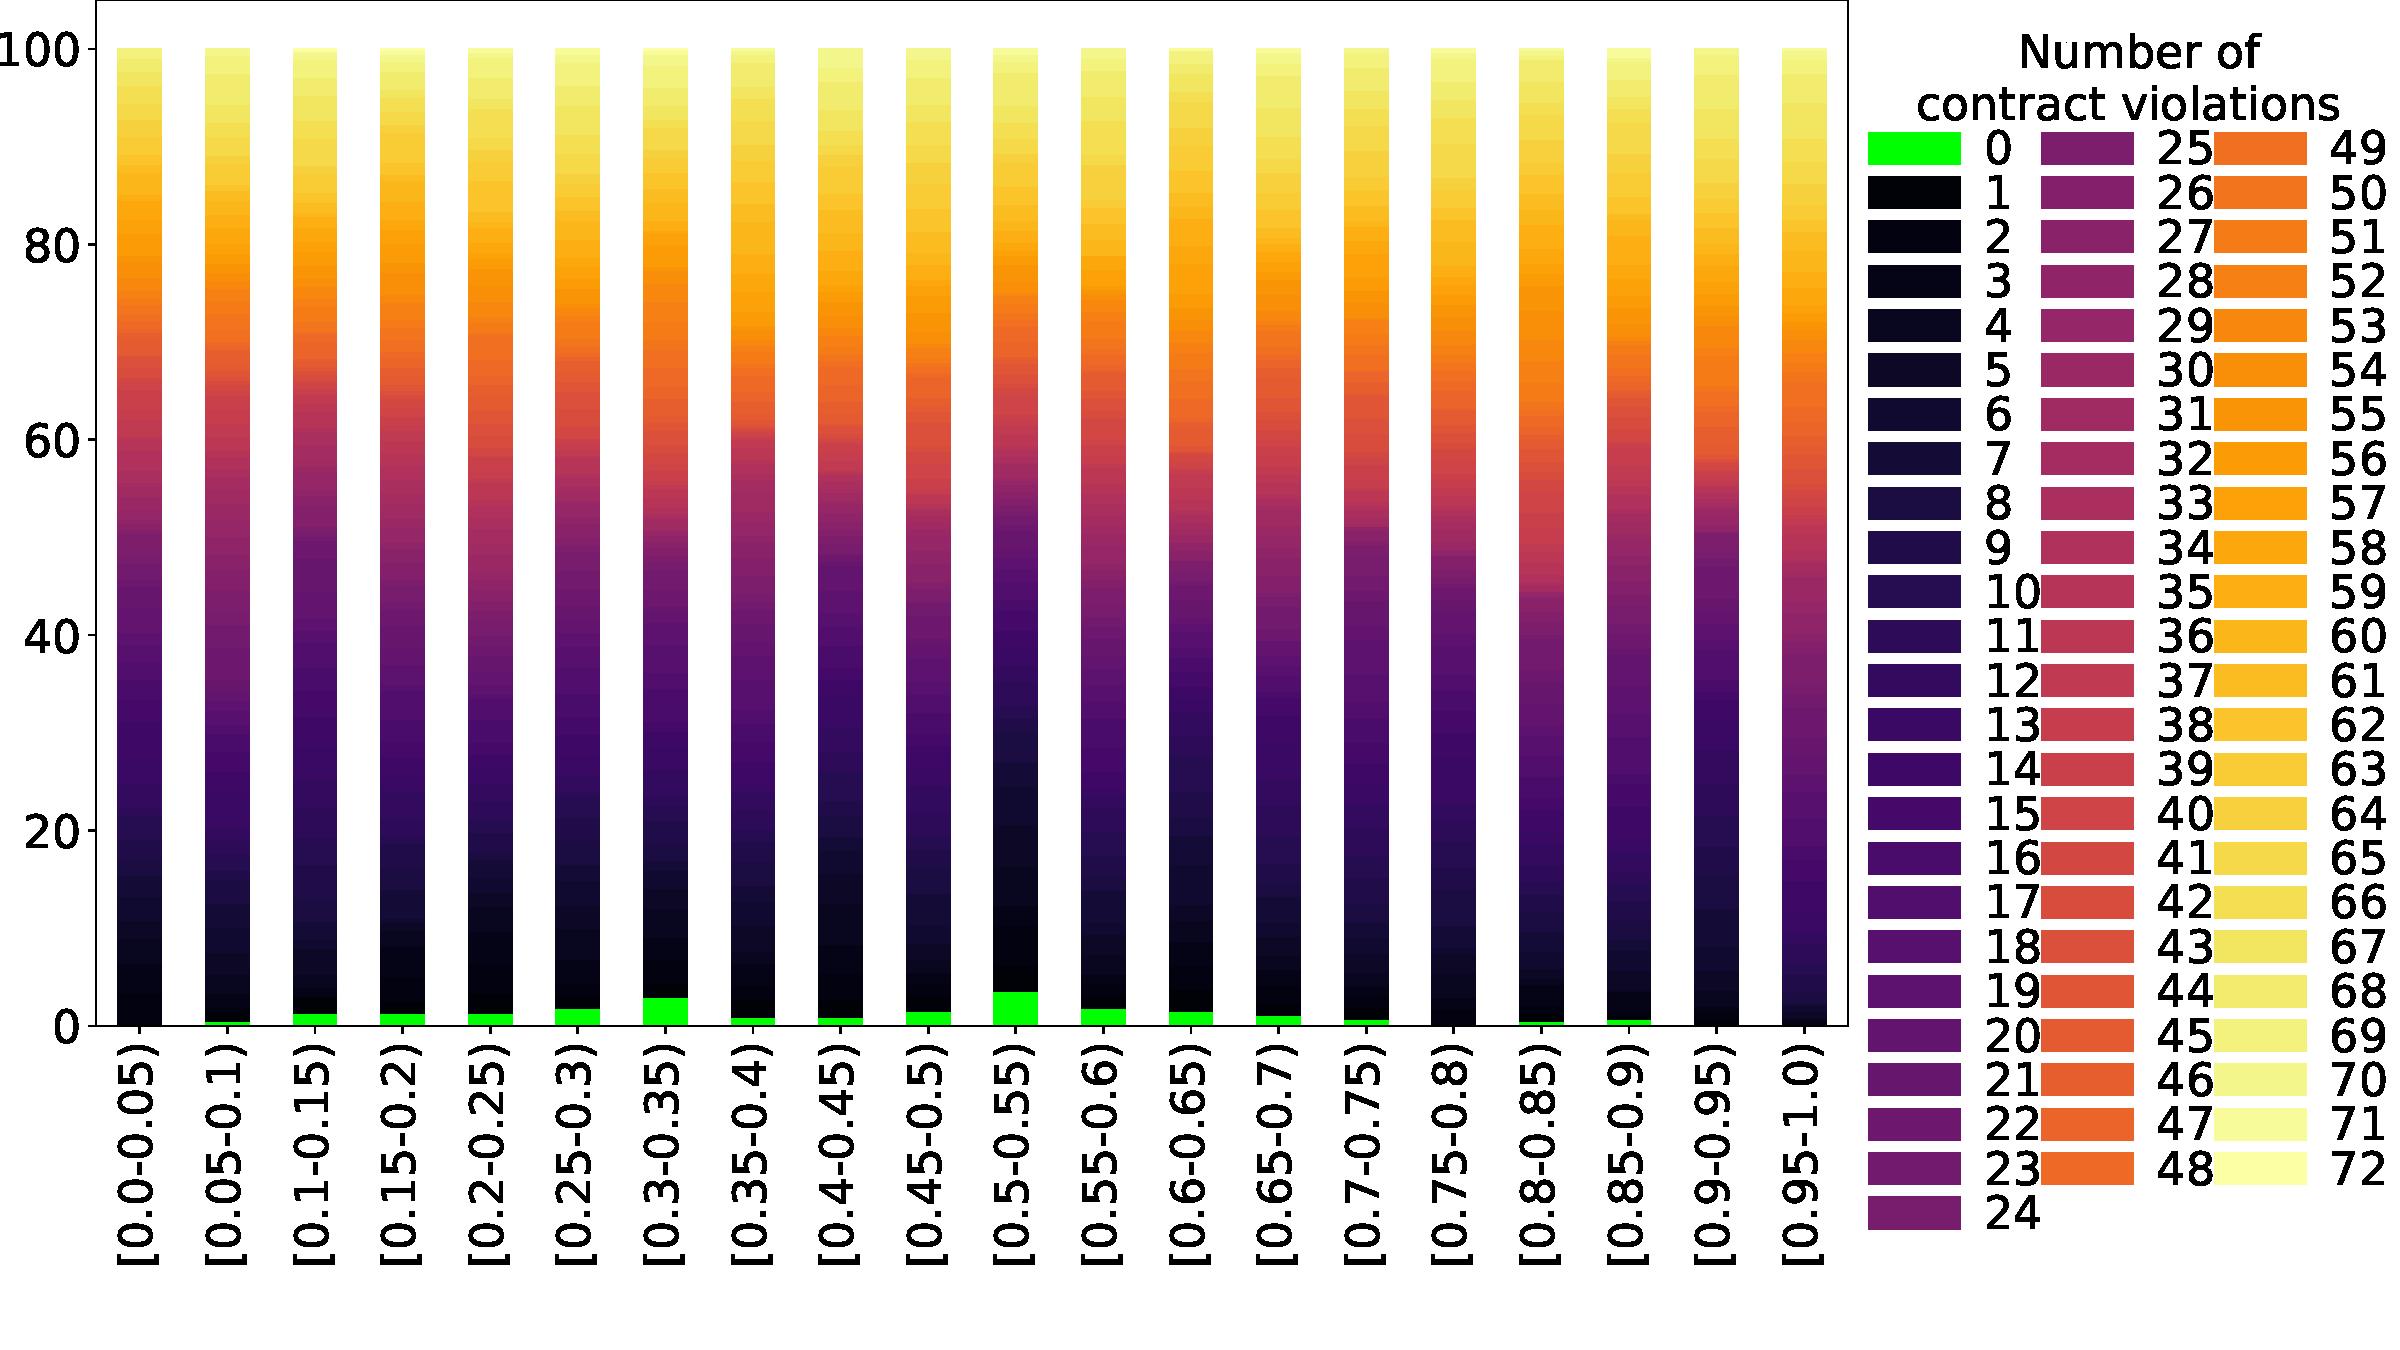
\includegraphics[width=\textwidth]{images/DistrValidityBig/crossoverOnRandomLevelProbability.pdf}
	\caption[crossoverOnRandomLevelProbability parameter values distribution for bigger problem]{crossoverOnRandomLevelProbability parameter values distribution for bigger problem}
	\label{fig:crossoverOnRandomLevelProbability_DistBig}
\end{figure}
\begin{figure}
	\centering
	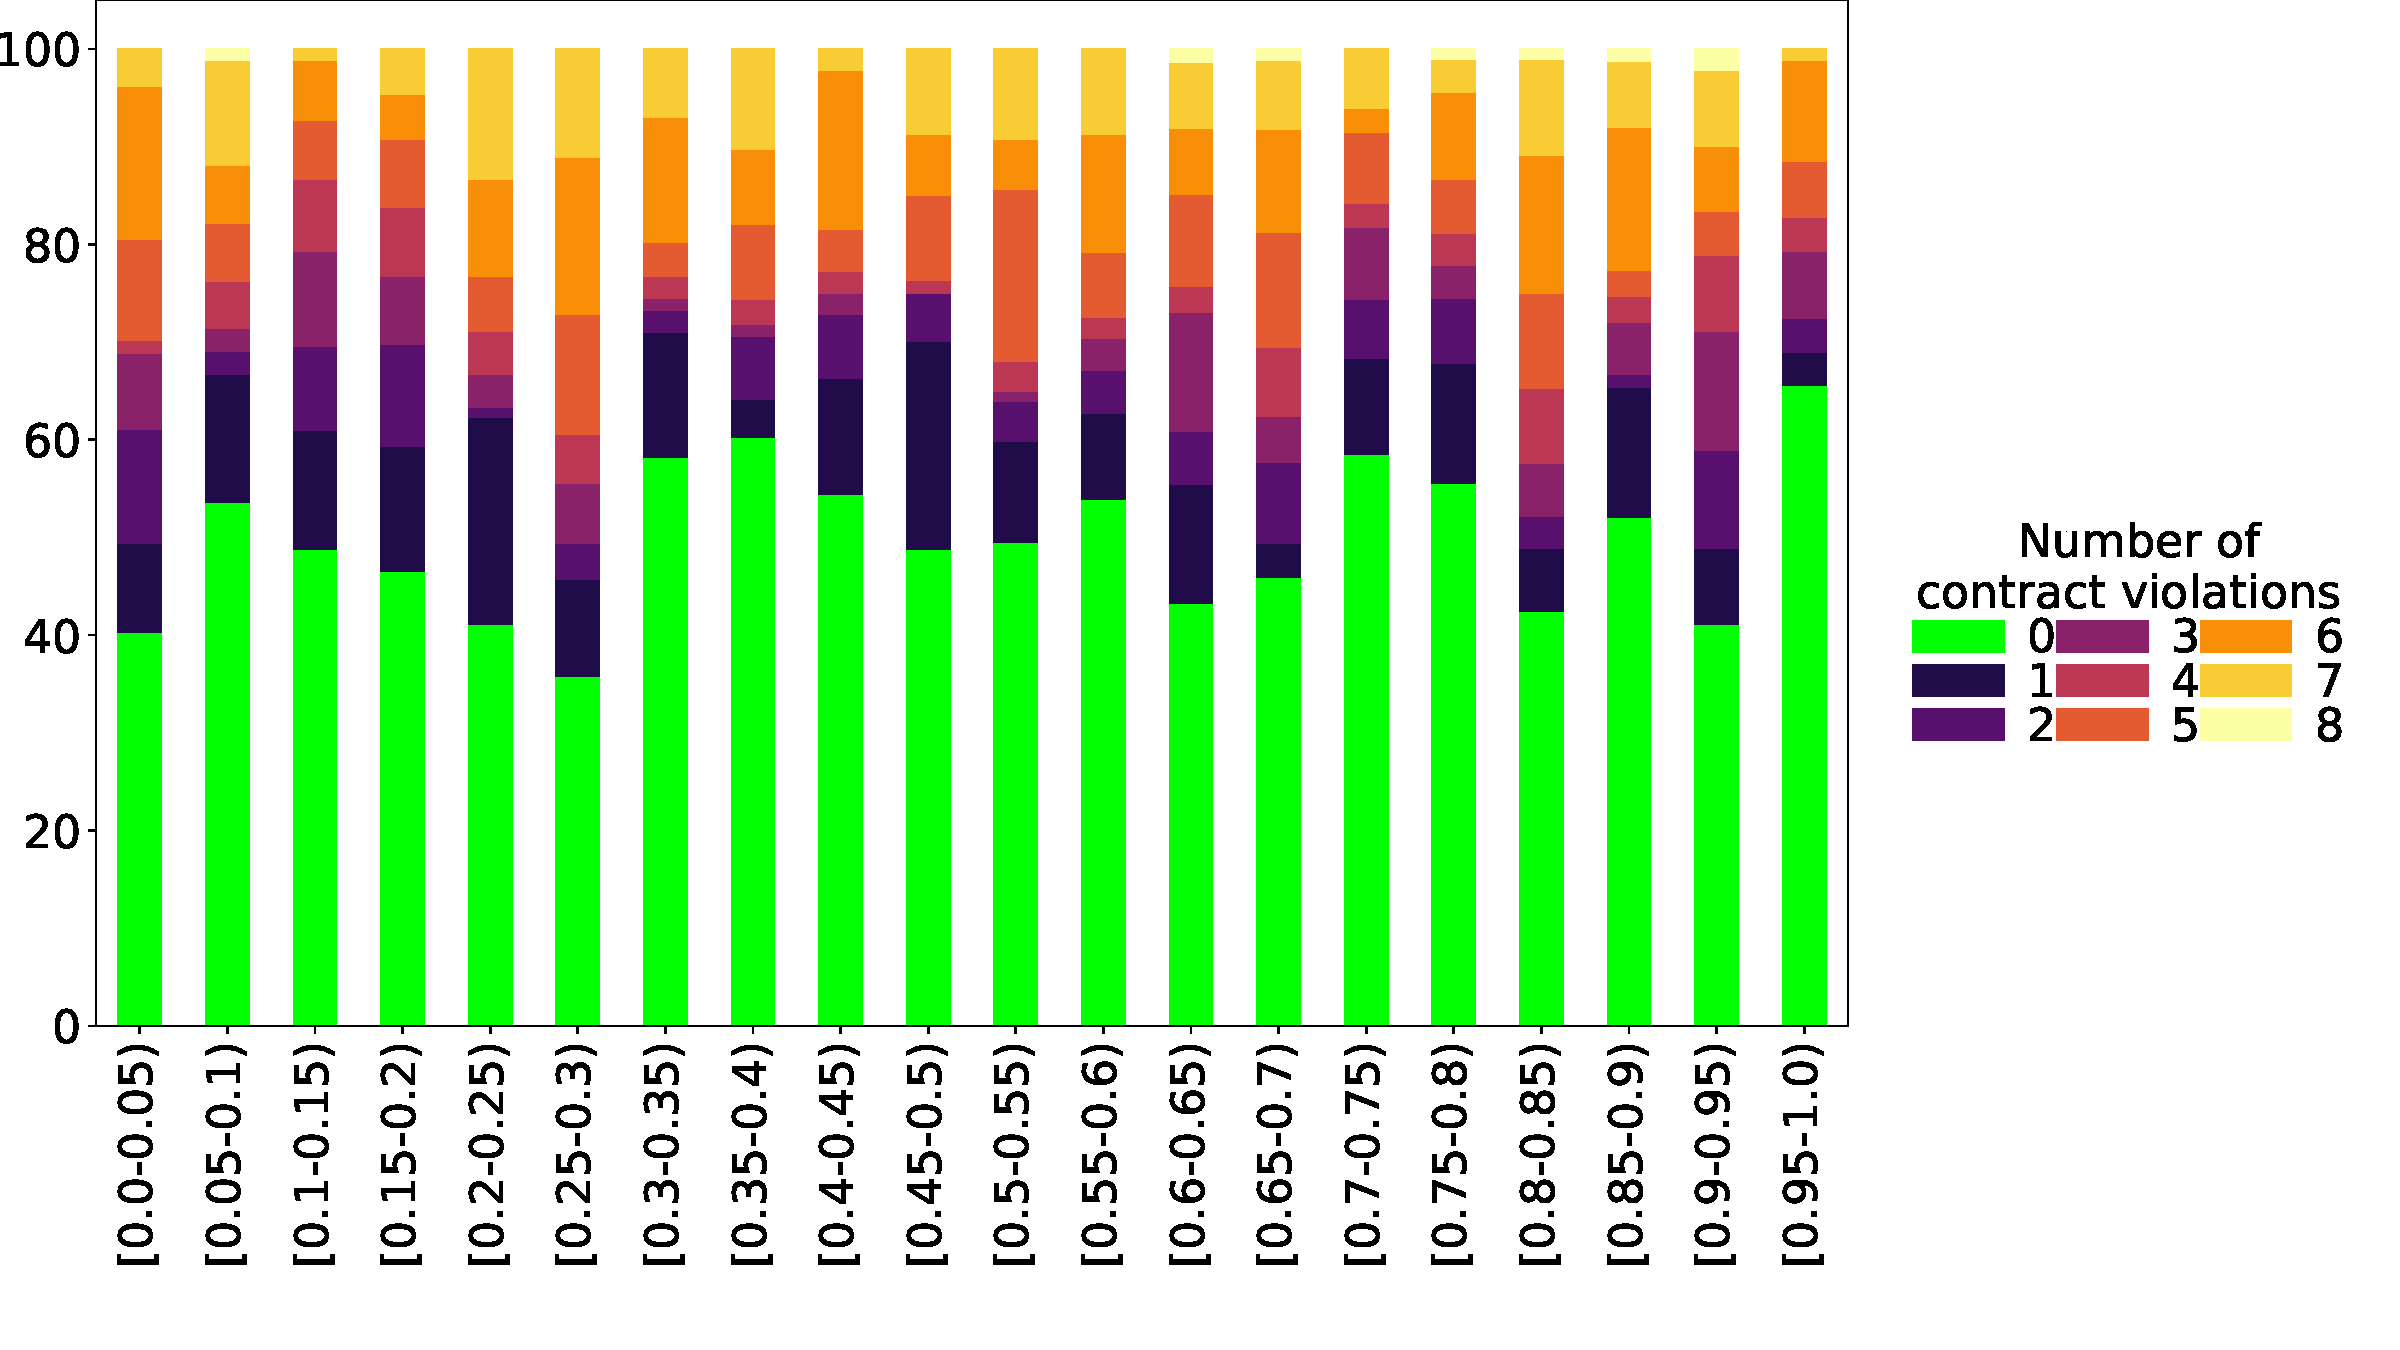
\includegraphics[width=\textwidth]{images/DistrValiditySmall/crossoverOnRandomLevelProbability.pdf}
	\caption[crossoverOnRandomLevelProbability parameter values distribution for smaller problem]{crossoverOnRandomLevelProbability parameter values distribution for smaller problem}
	\label{fig:crossoverOnRandomLevelProbability_DistSmall}
\end{figure}
\begin{figure}
	\centering
	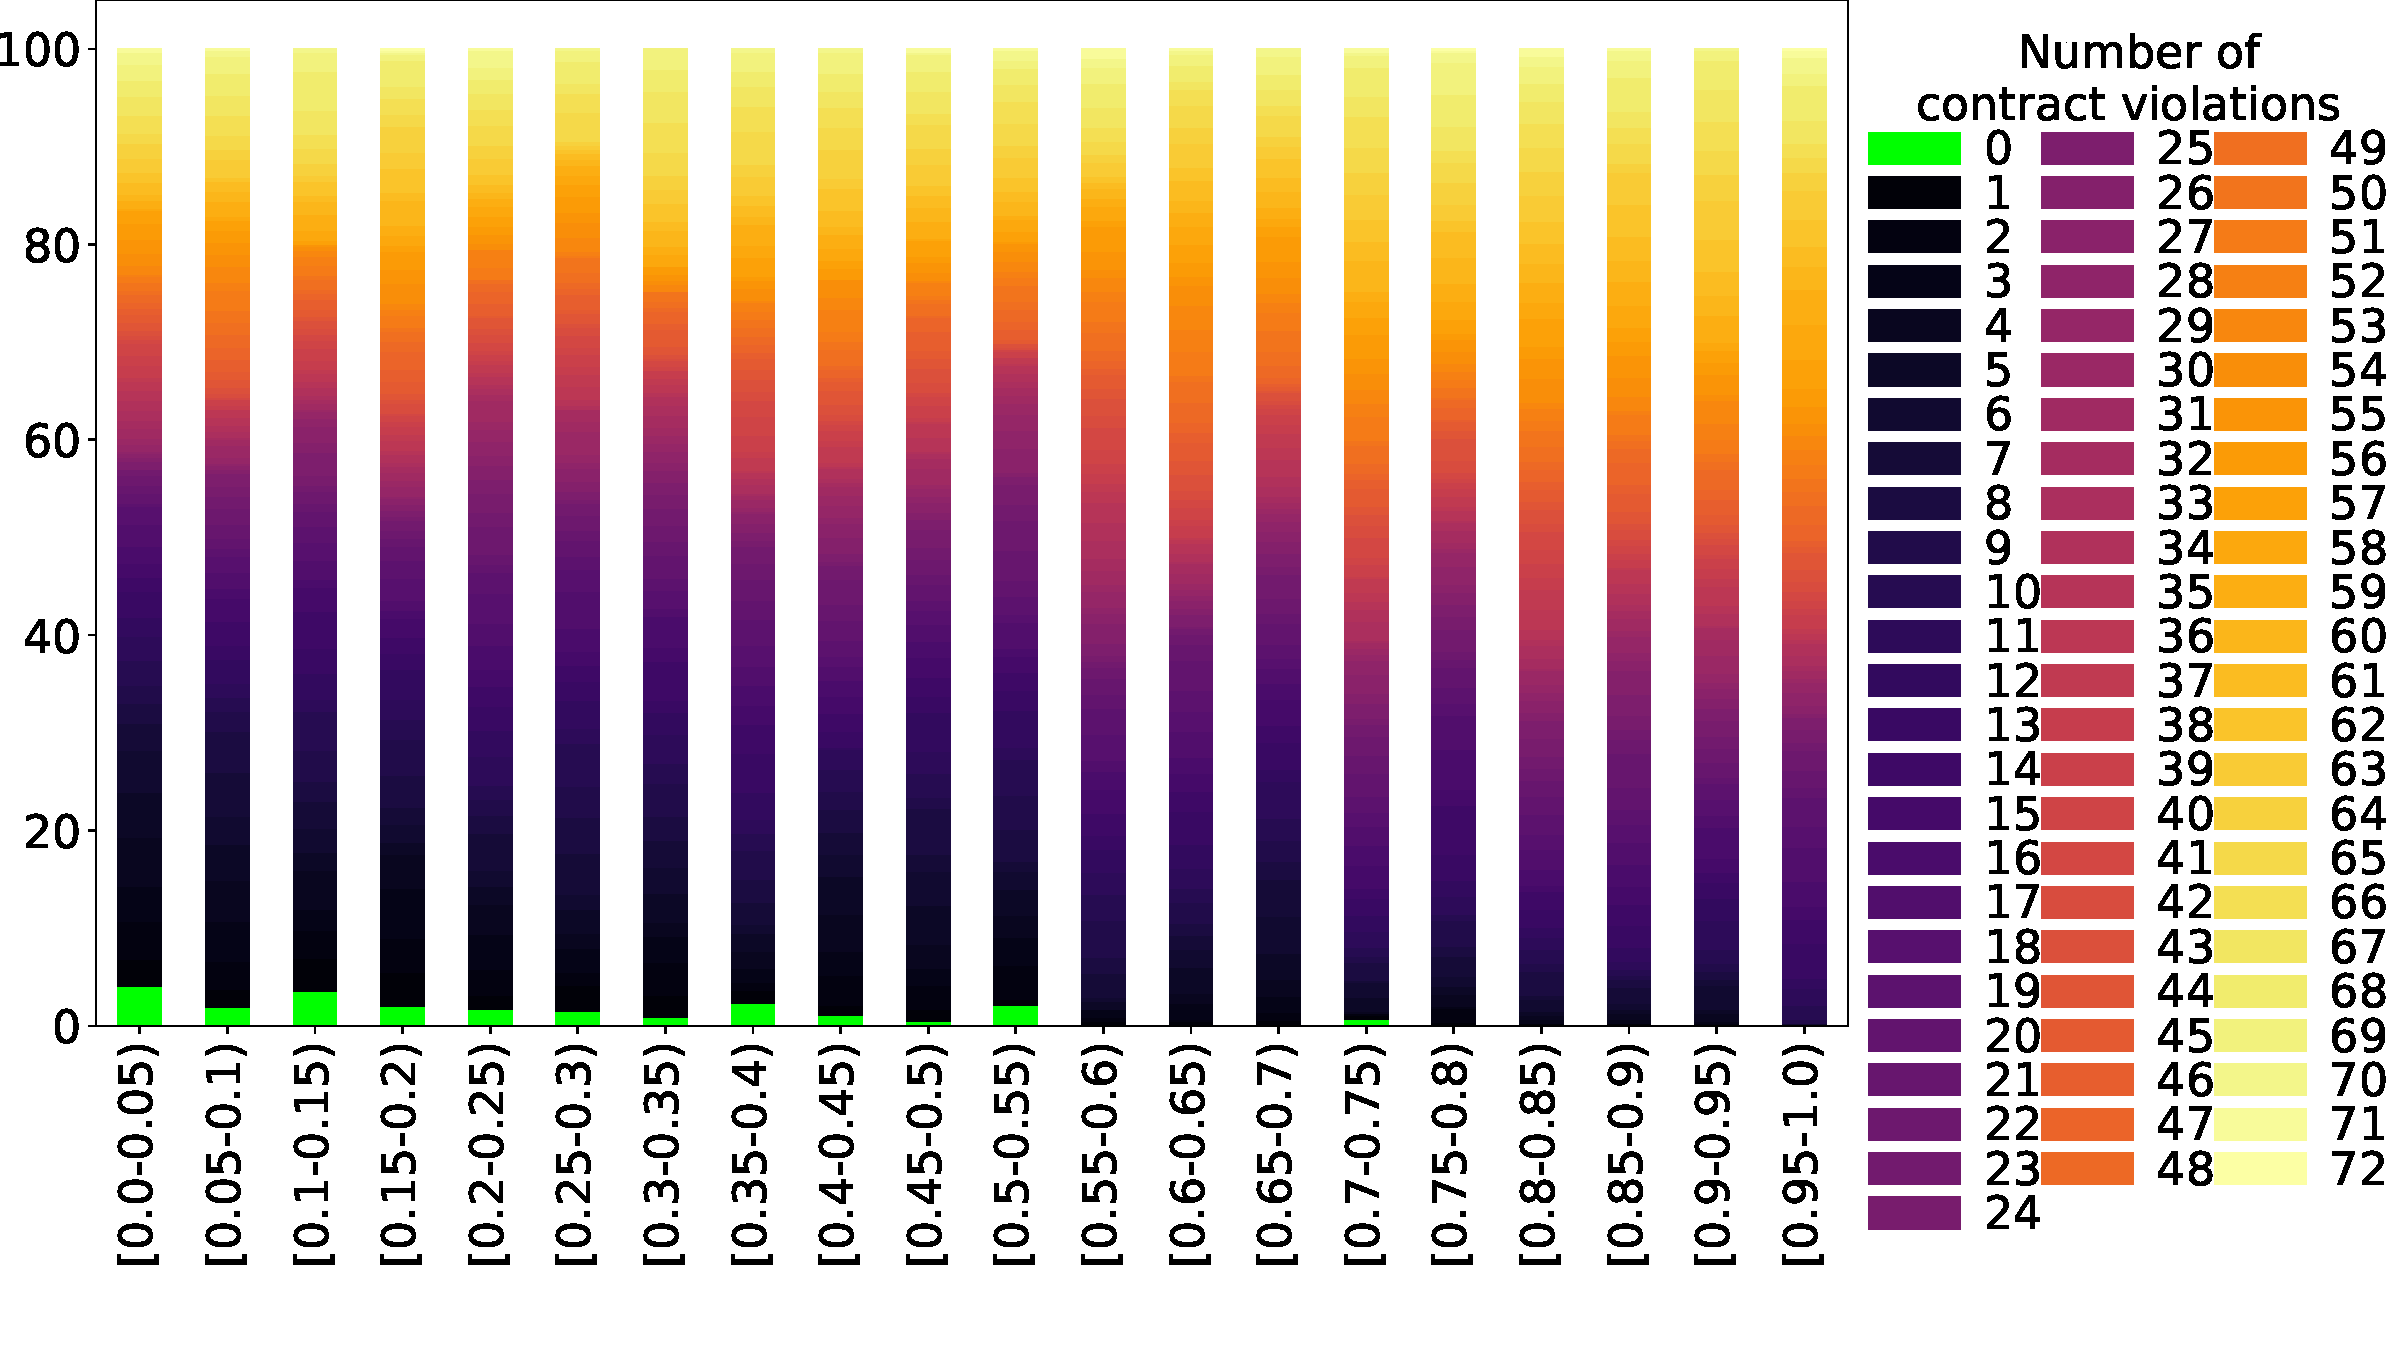
\includegraphics[width=\textwidth]{images/DistrValidityBig/crossoverOnRandomRequestProbability.pdf}
	\caption[crossoverOnRandomRequestProbability parameter values distribution for bigger problem]{crossoverOnRandomRequestProbability parameter values distribution for bigger problem}
	\label{fig:crossoverOnRandomRequestProbability_DistBig}
\end{figure}
\begin{figure}
	\centering
	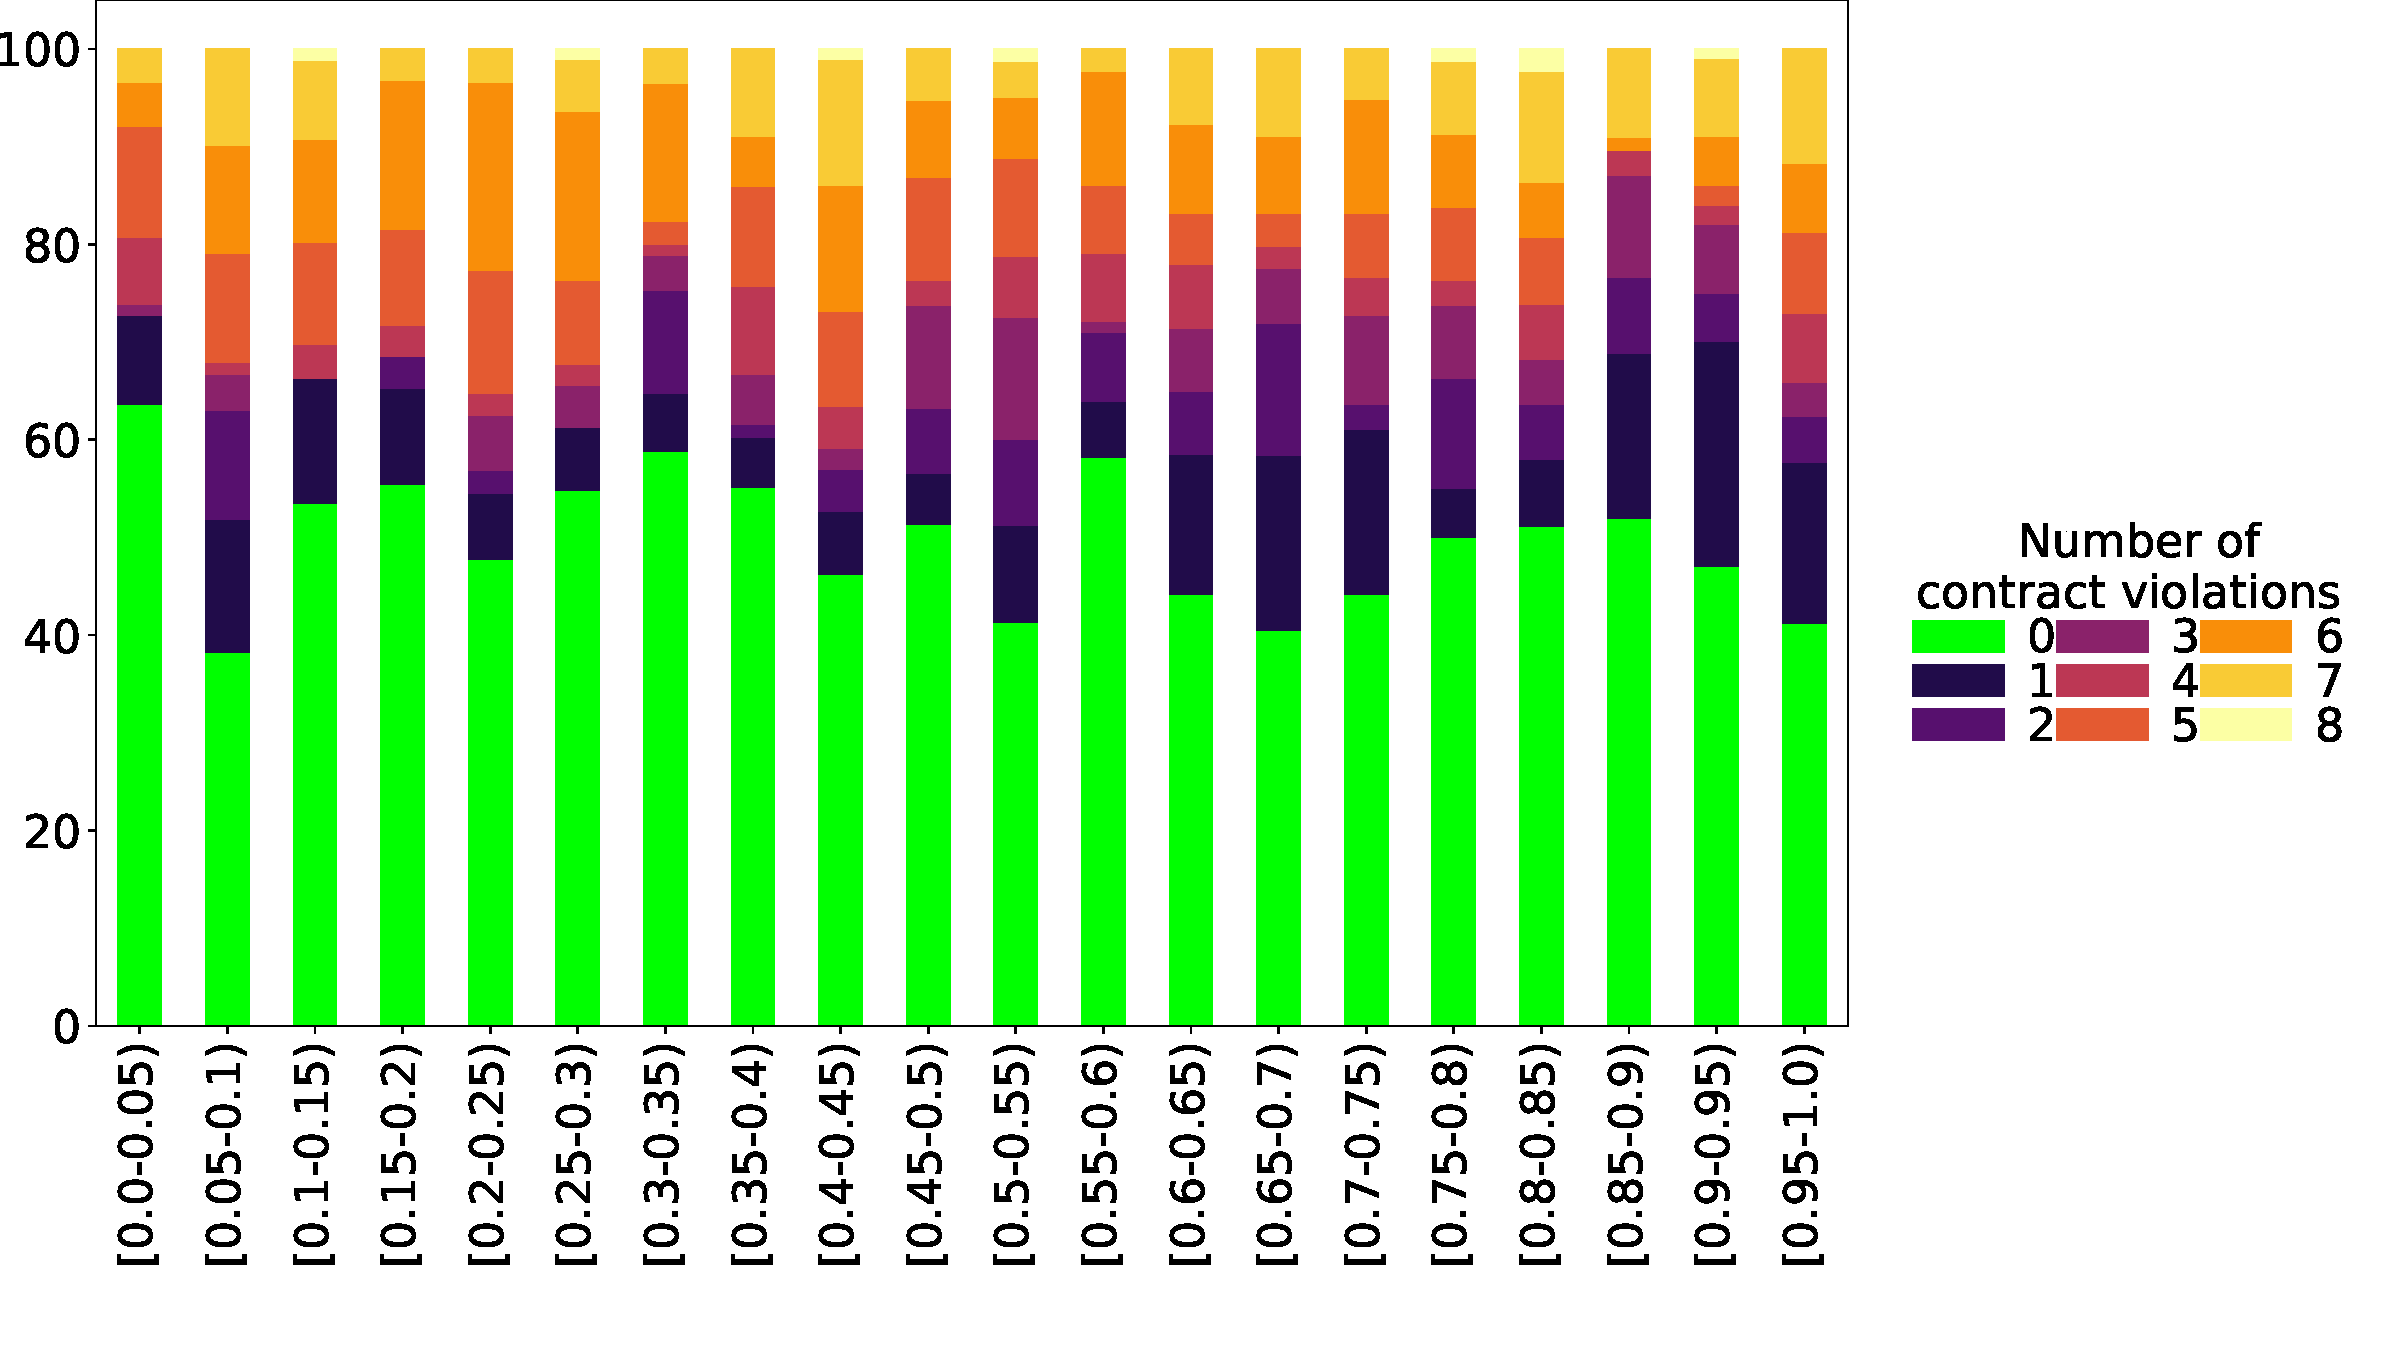
\includegraphics[width=\textwidth]{images/DistrValiditySmall/crossoverOnRandomRequestProbability.pdf}
	\caption[crossoverOnRandomRequestProbability parameter values distribution for smaller problem]{crossoverOnRandomRequestProbability parameter values distribution for smaller problem}       
	\label{fig:crossoverOnRandomRequestProbability_DistSmall}
\end{figure}
\begin{figure}
	\centering
	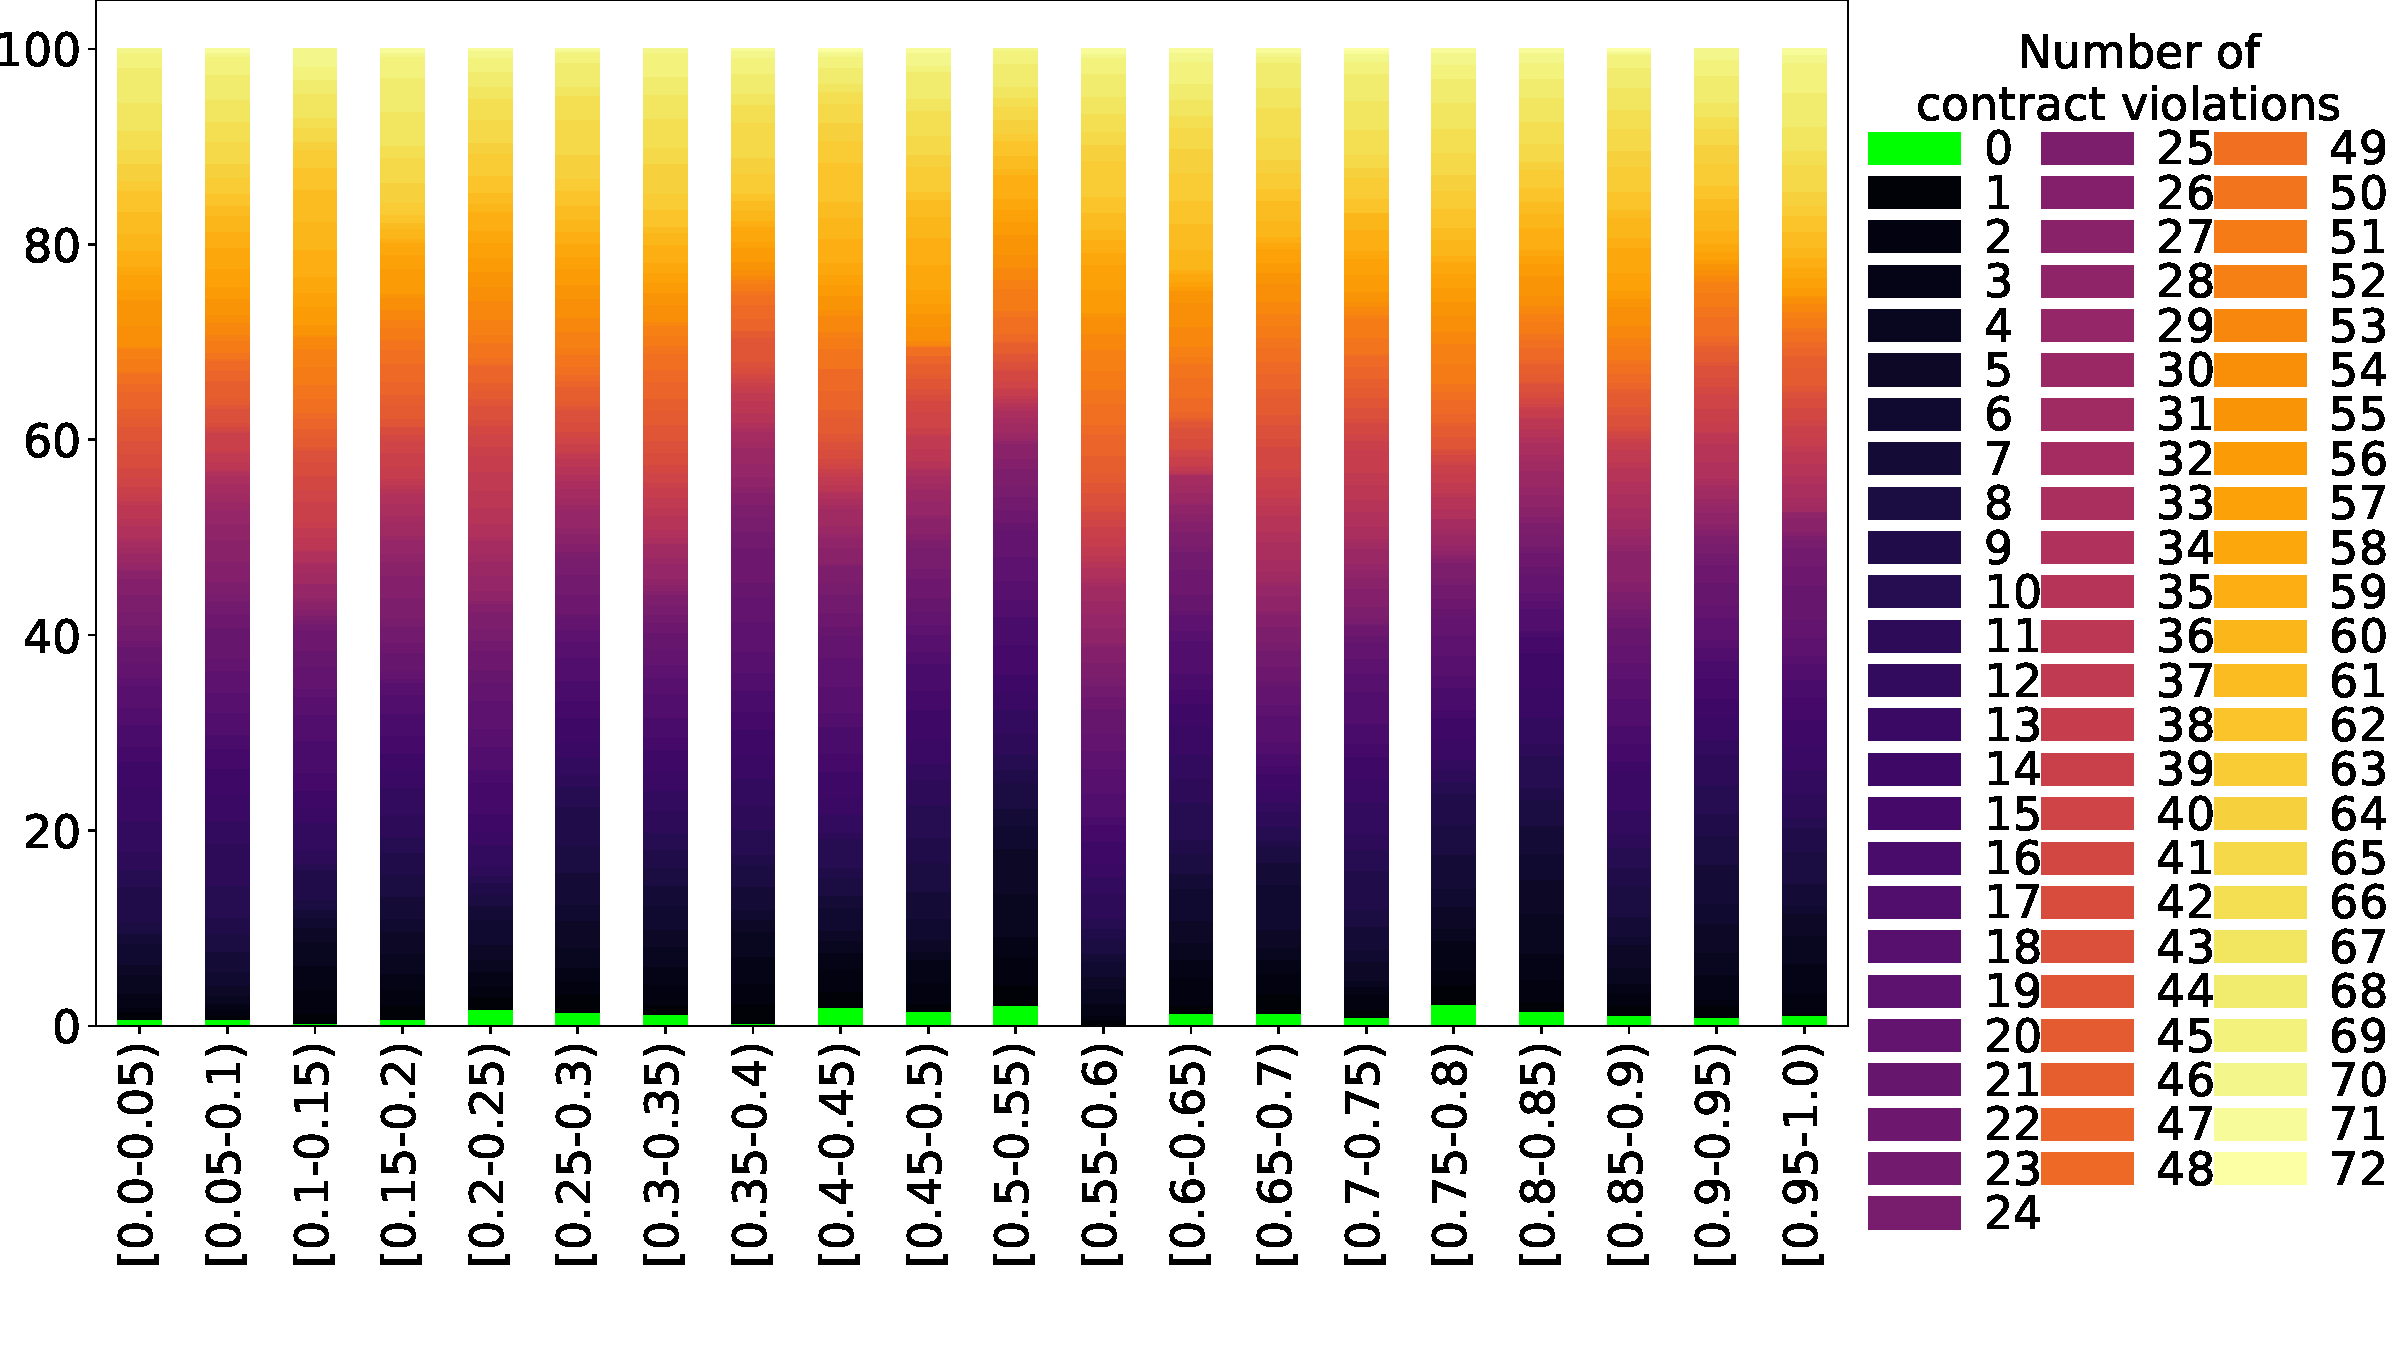
\includegraphics[width=\textwidth]{images/DistrValidityBig/mutationOnRandomChildProbability.pdf}
	\caption[mutationOnRandomChildProbability parameter values distribution for bigger problem]{mutationOnRandomChildProbability parameter values distribution for bigger problem}
	\label{fig:mutationOnRandomChildProbability_DistBig}
\end{figure}
\begin{figure}
	\centering
	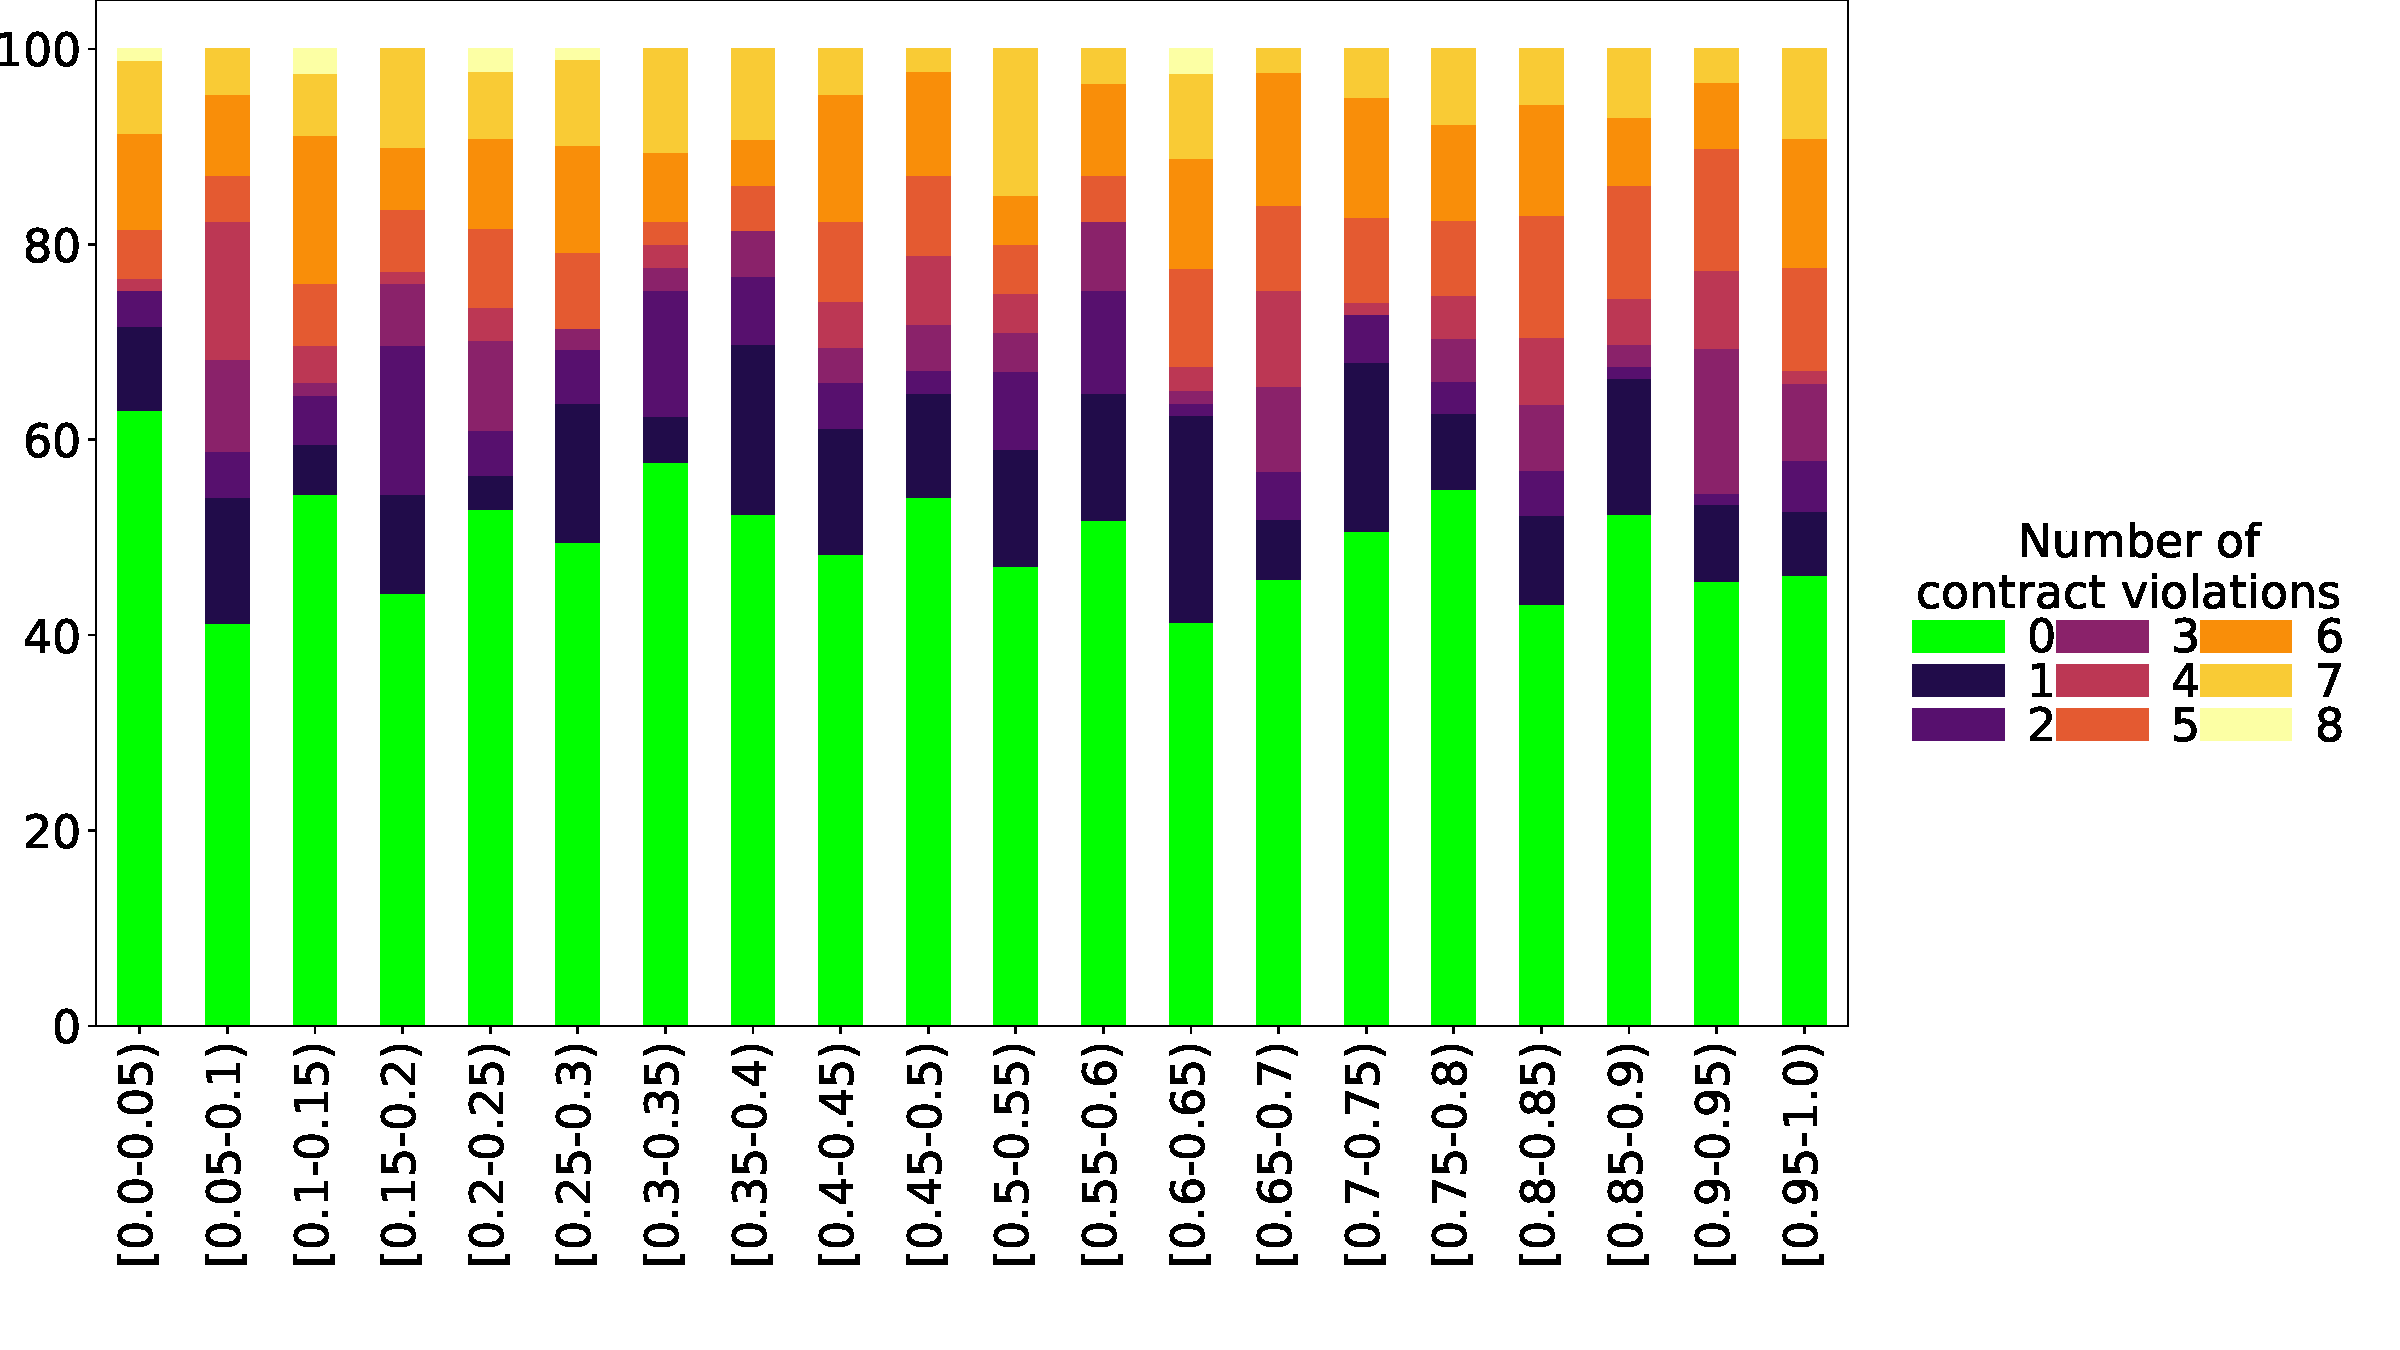
\includegraphics[width=\textwidth]{images/DistrValiditySmall/mutationOnRandomChildProbability.pdf}
	\caption[mutationOnRandomChildProbability parameter values distribution for smaller problem]{mutationOnRandomChildProbability parameter values distribution for smaller problem}
	\label{fig:mutationOnRandomChildProbability_DistSmall}
\end{figure}
\begin{figure}
	\centering
	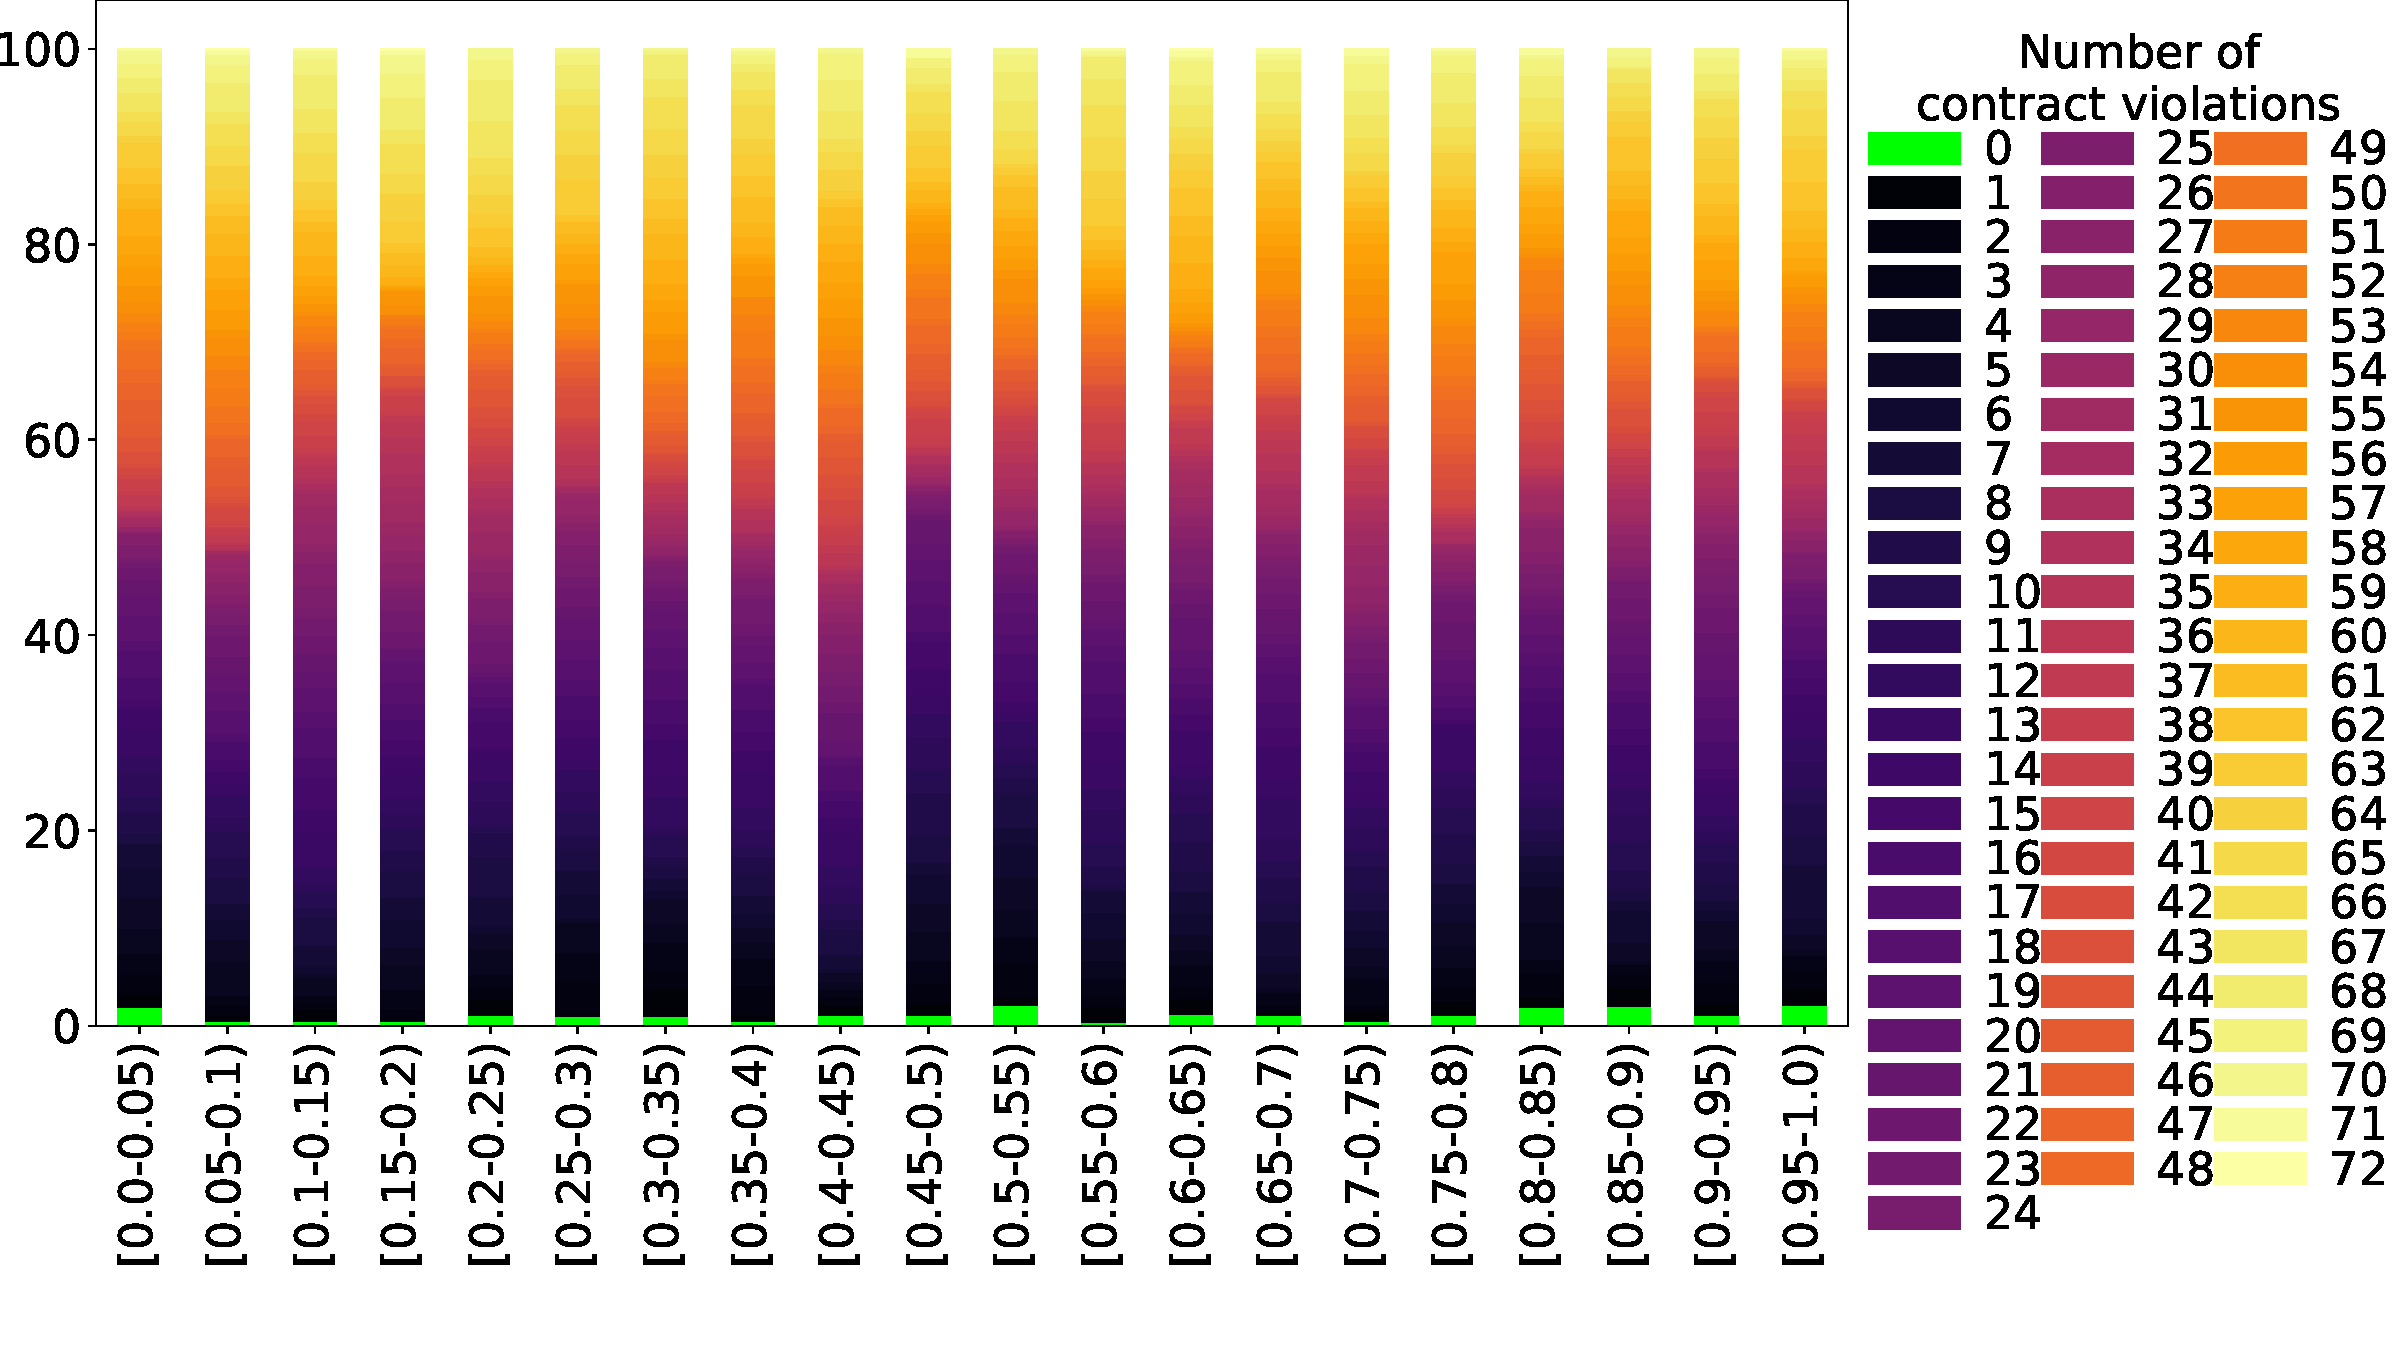
\includegraphics[width=\textwidth]{images/DistrValidityBig/mutationOnRandomLevelProbability.pdf}
	\caption[mutationOnRandomLevelProbability parameter values distribution for bigger problem]{mutationOnRandomLevelProbability parameter values distribution for bigger problem}
	\label{fig:mutationOnRandomLevelProbability_DistBig}
\end{figure}
\begin{figure}
	\centering
	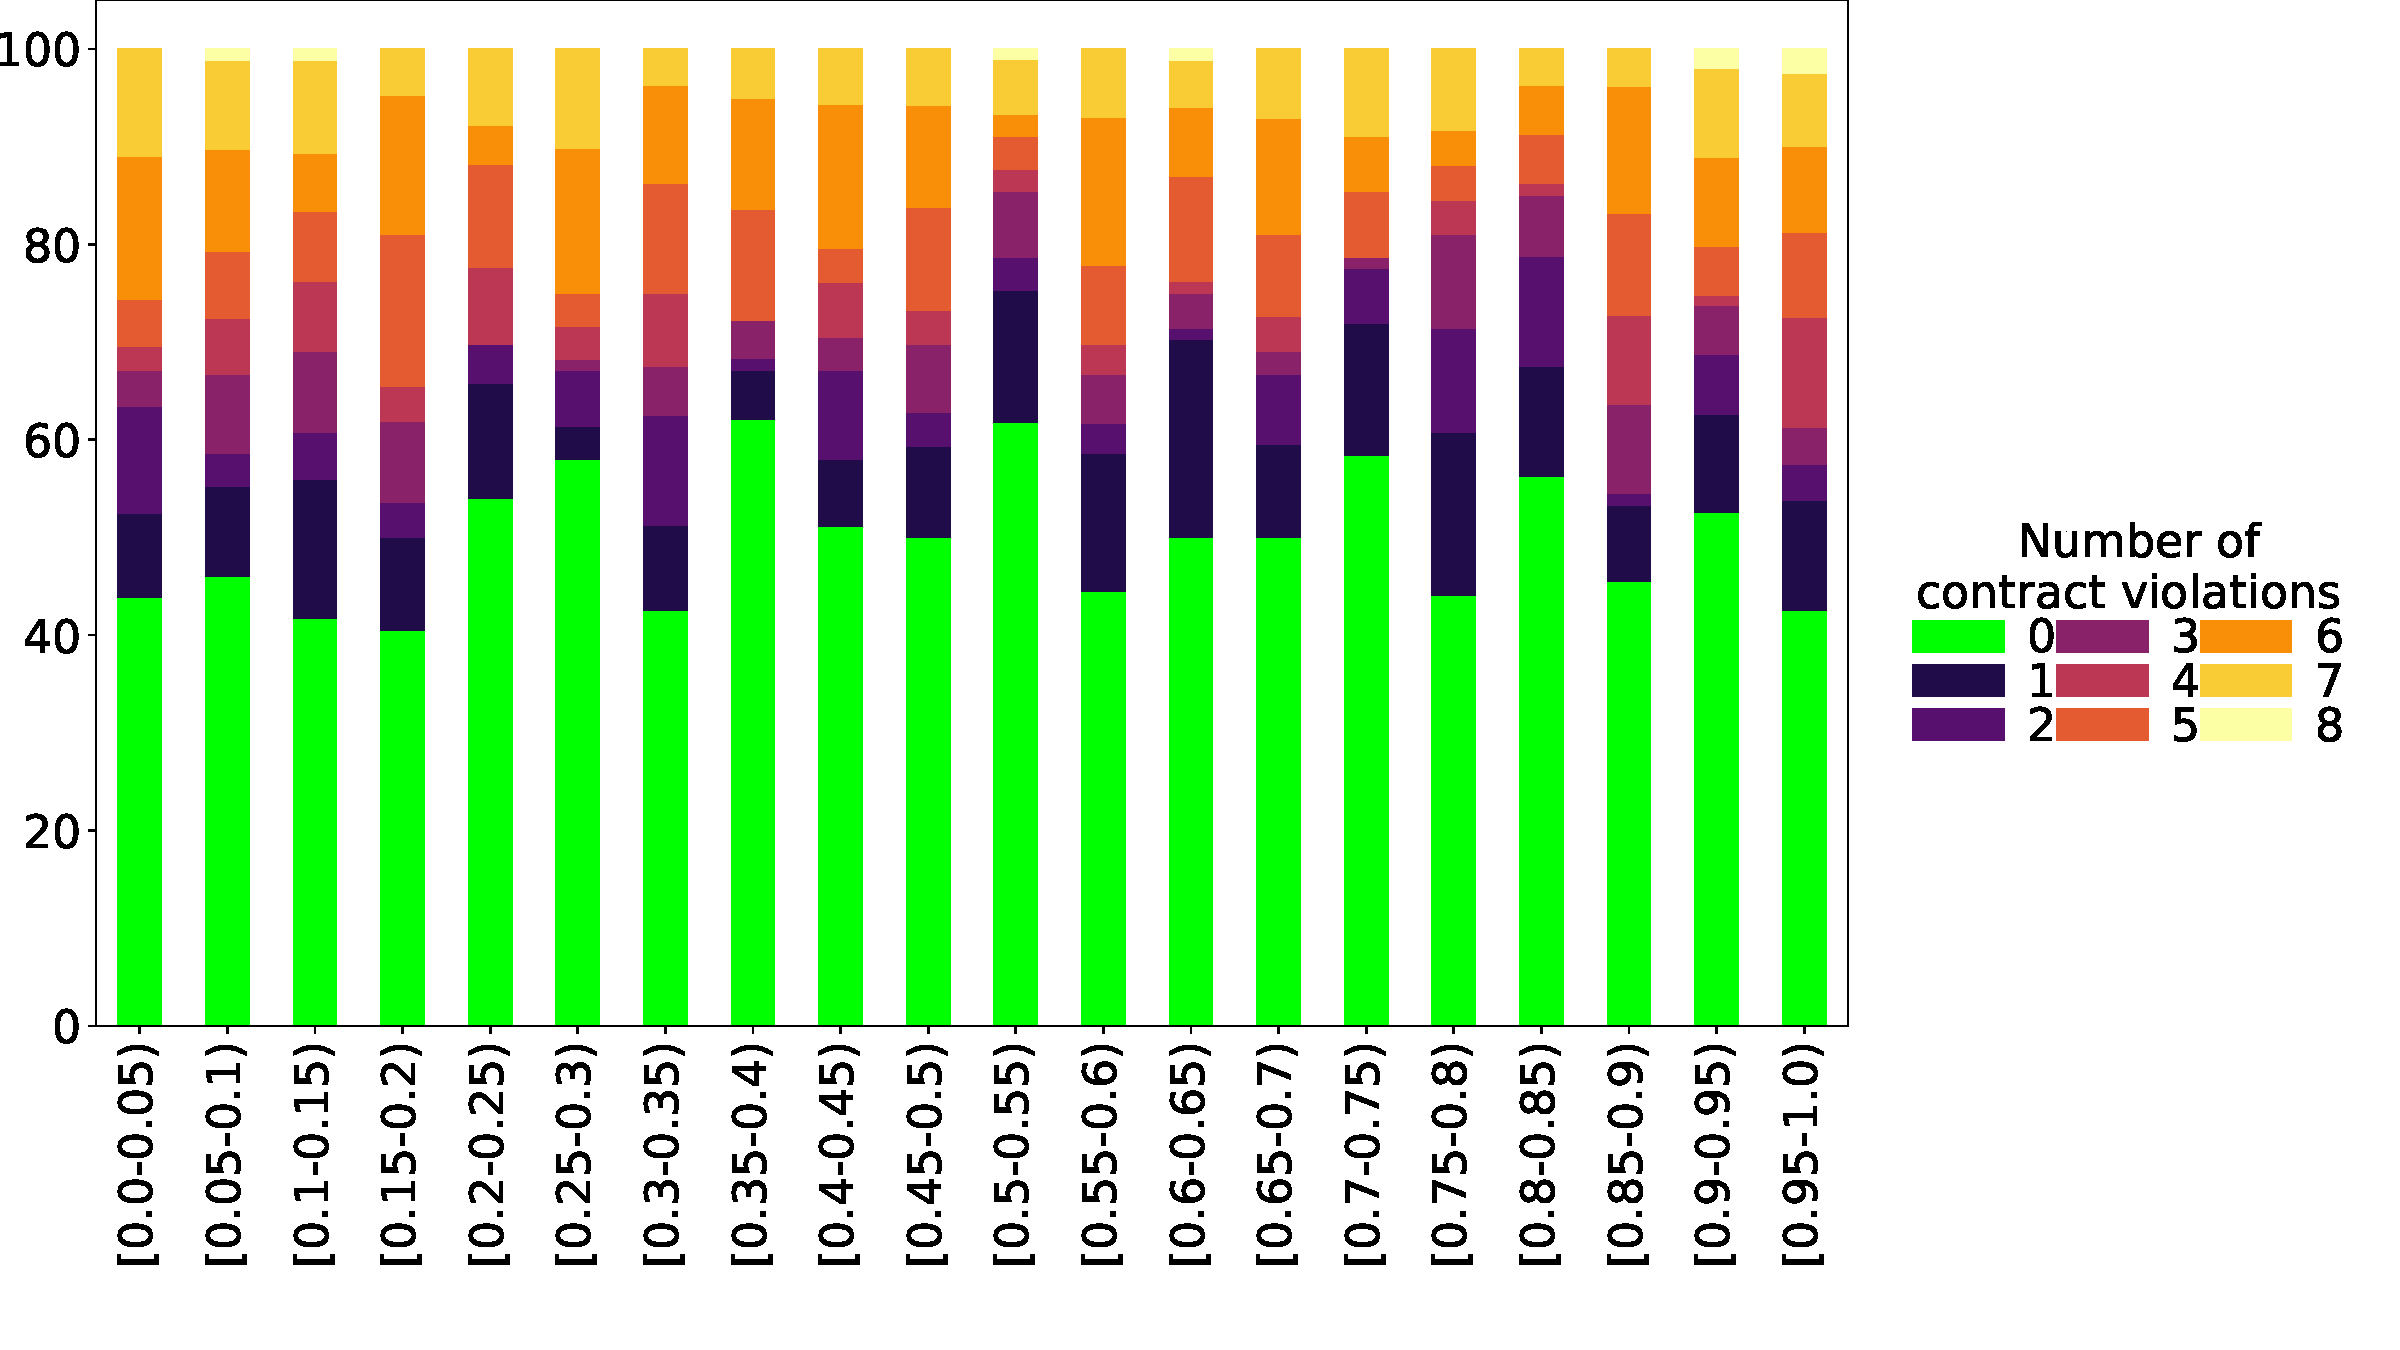
\includegraphics[width=\textwidth]{images/DistrValiditySmall/mutationOnRandomLevelProbability.pdf}
	\caption[mutationOnRandomLevelProbability parameter values distribution for smaller problem]{mutationOnRandomLevelProbability parameter values distribution for smaller problem}
	\label{fig:mutationOnRandomLevelProbability_DistSmall}
\end{figure}
\begin{figure}
	\centering
	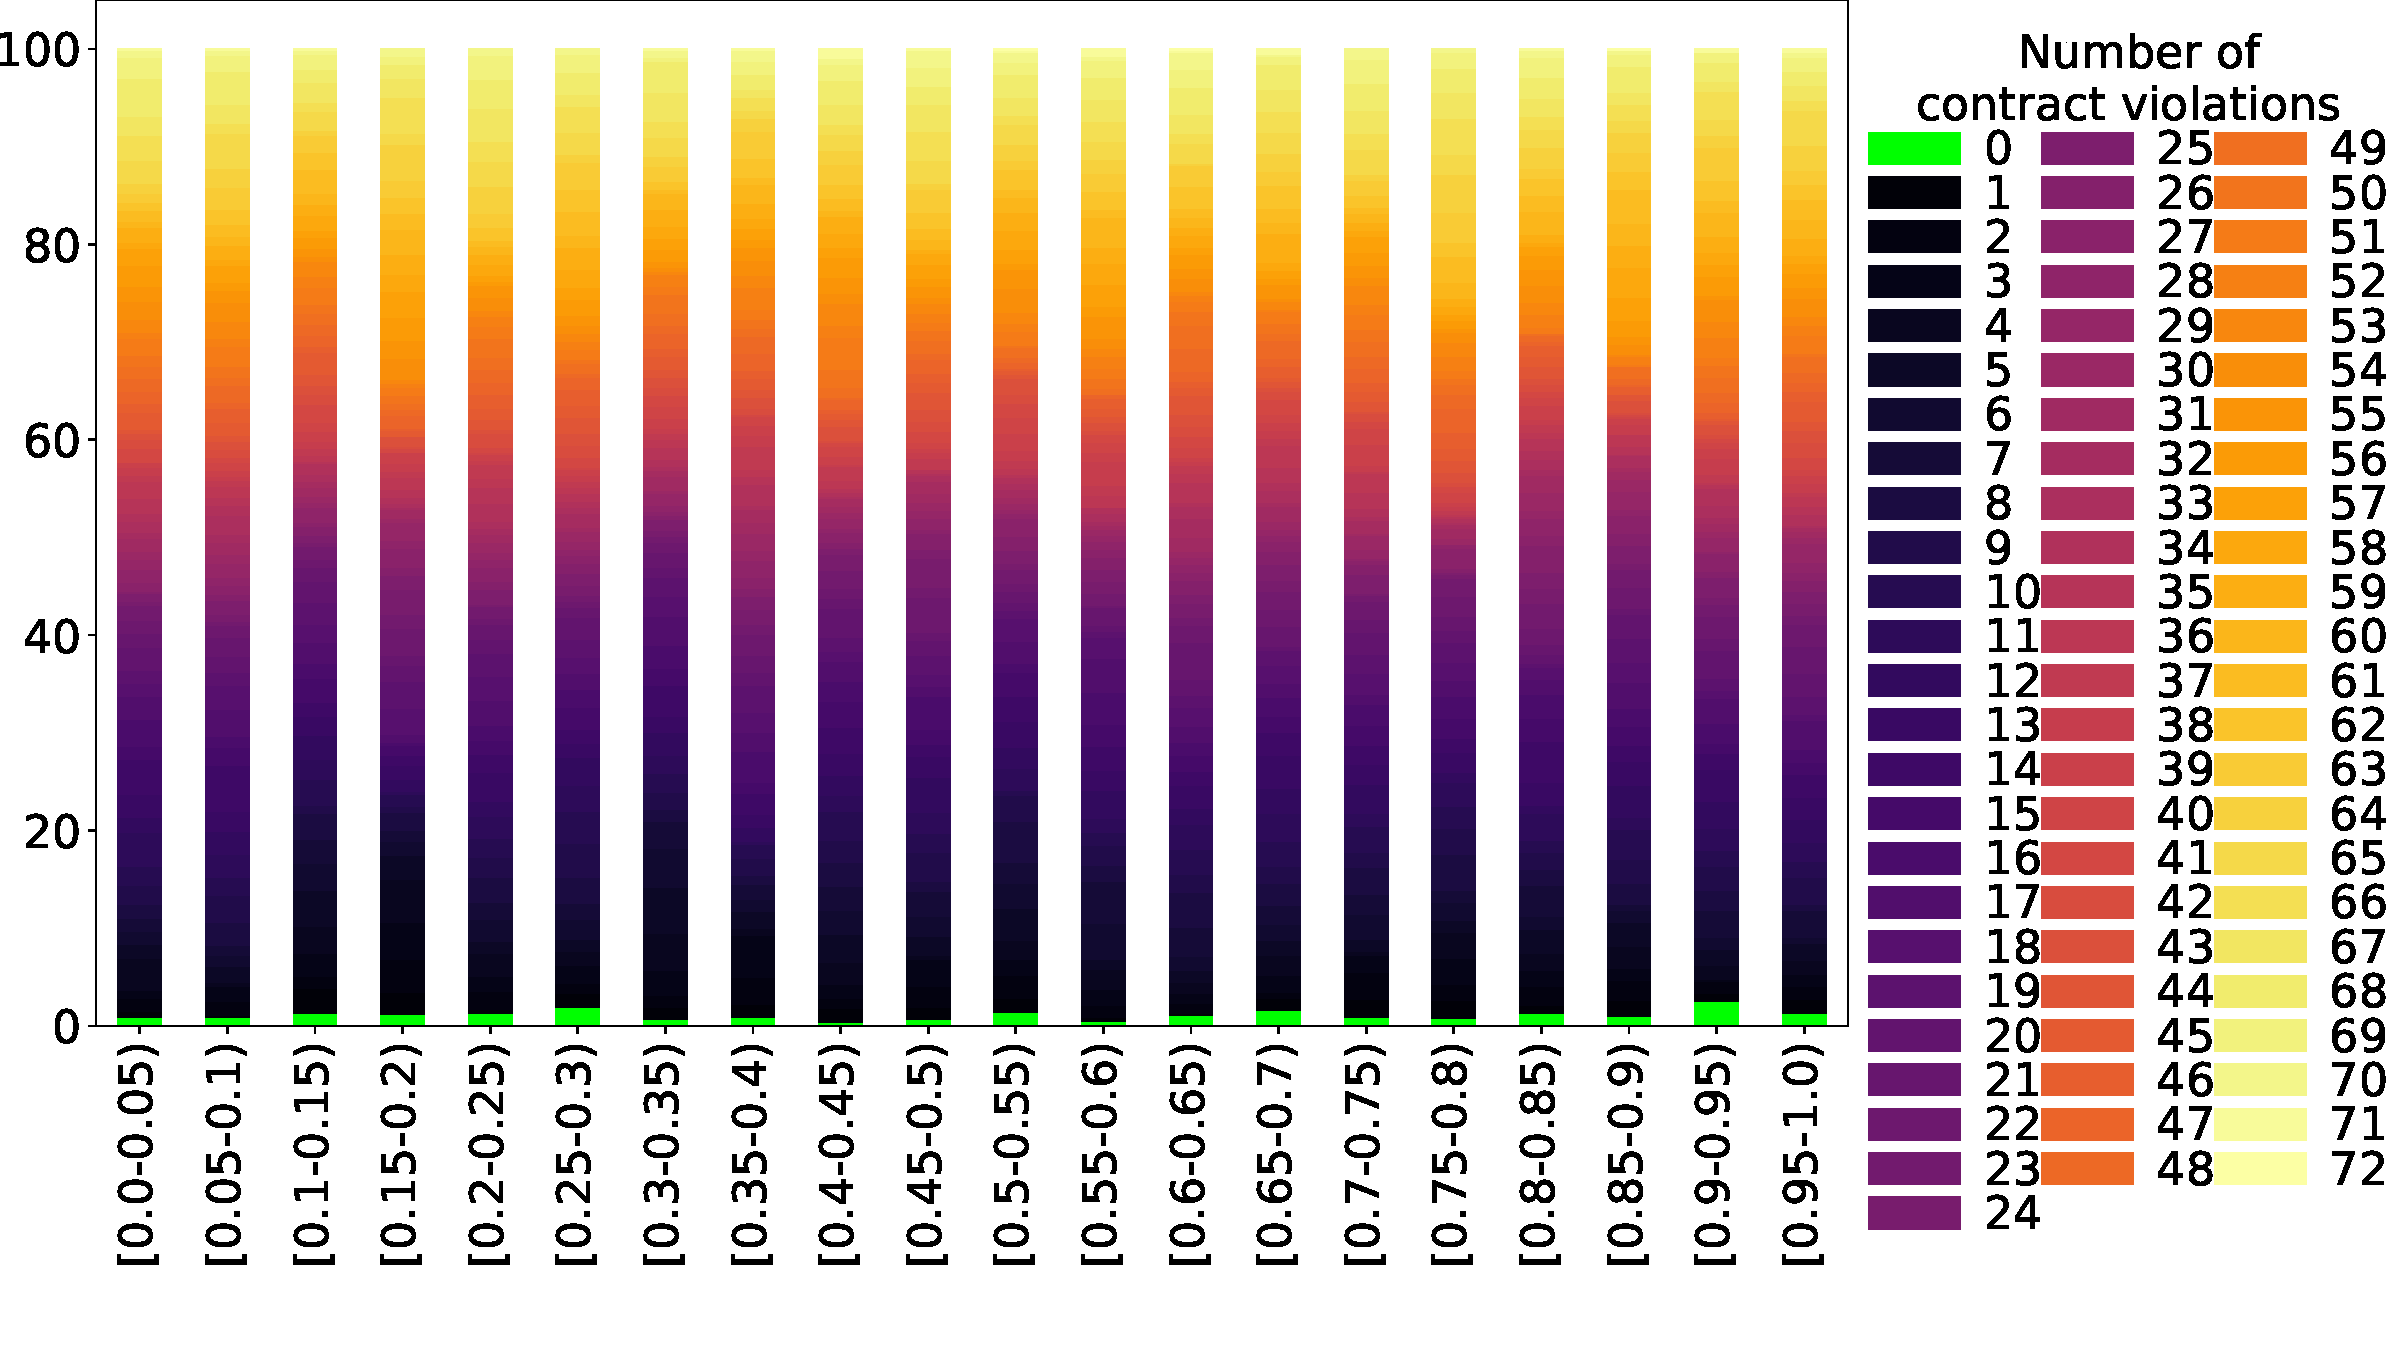
\includegraphics[width=\textwidth]{images/DistrValidityBig/evaluatorValidityWeight.pdf}
	\caption[evaluatorValidityWeight parameter values distribution for bigger problem]{evaluatorValidityWeight parameter values distribution for bigger problem}
	\label{fig:evaluatorValidityWeight_DistBig}
\end{figure}
\begin{figure}
	\centering
	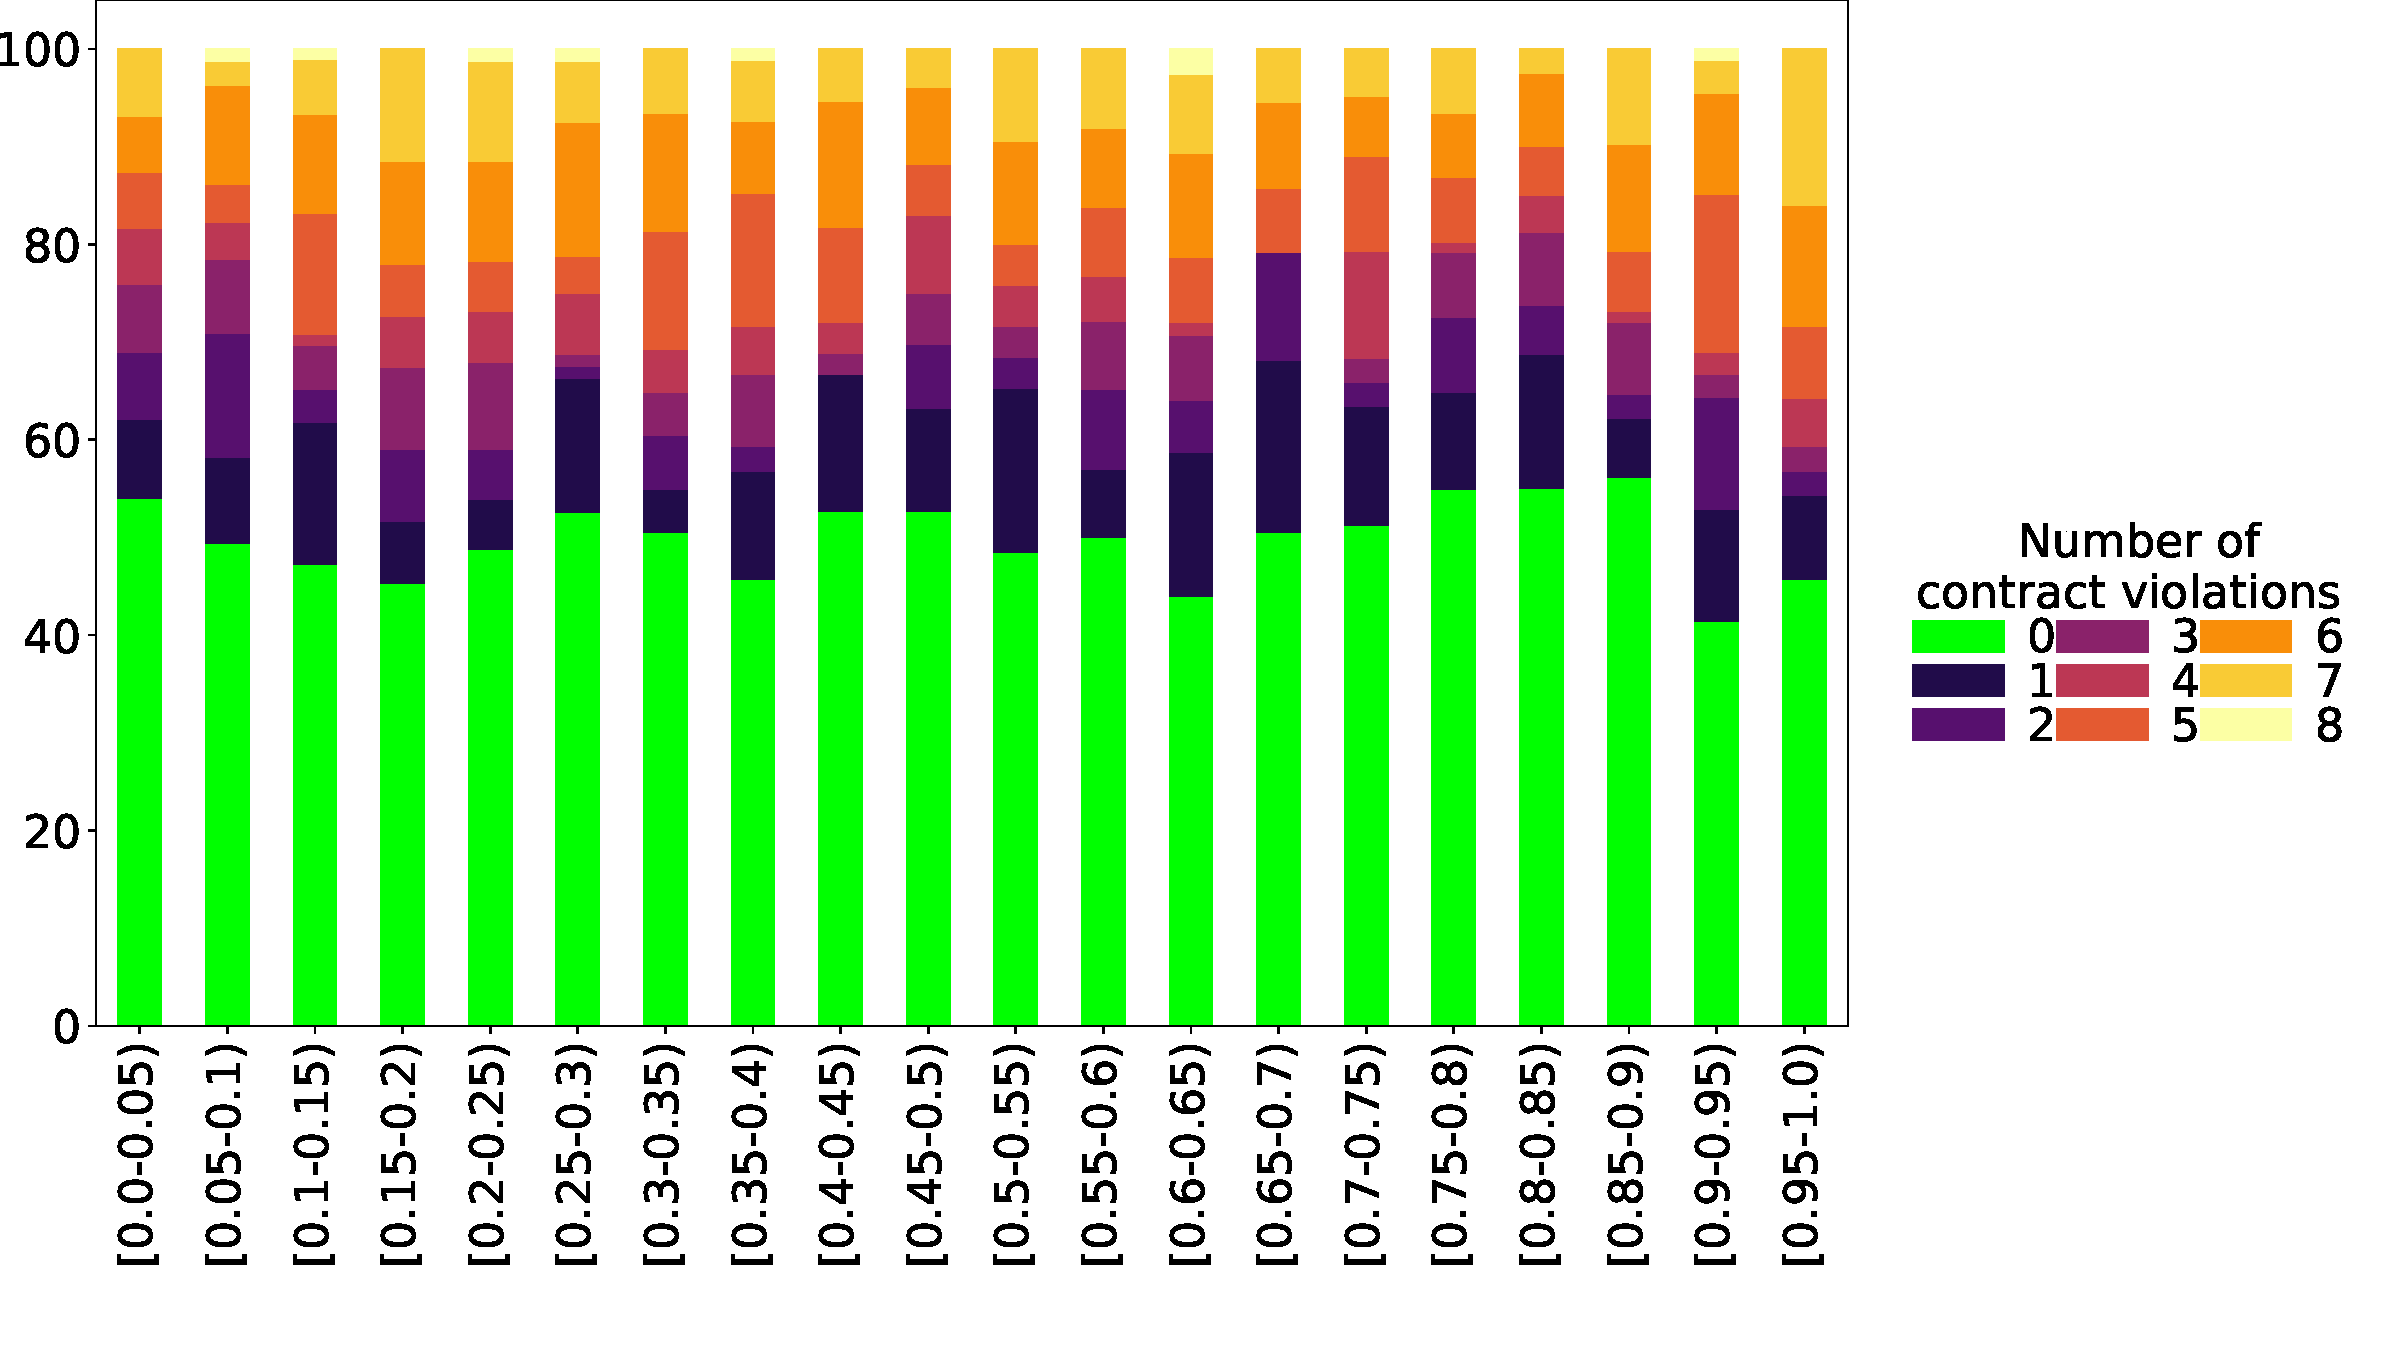
\includegraphics[width=\textwidth]{images/DistrValiditySmall/evaluatorValidityWeight.pdf}
	\caption[evaluatorValidityWeight parameter values distribution for smaller problem]{evaluatorValidityWeight parameter values distribution for smaller problem}
	\label{fig:evaluatorValidityWeight_DistSmall}
\end{figure}
\begin{figure}
	\centering
	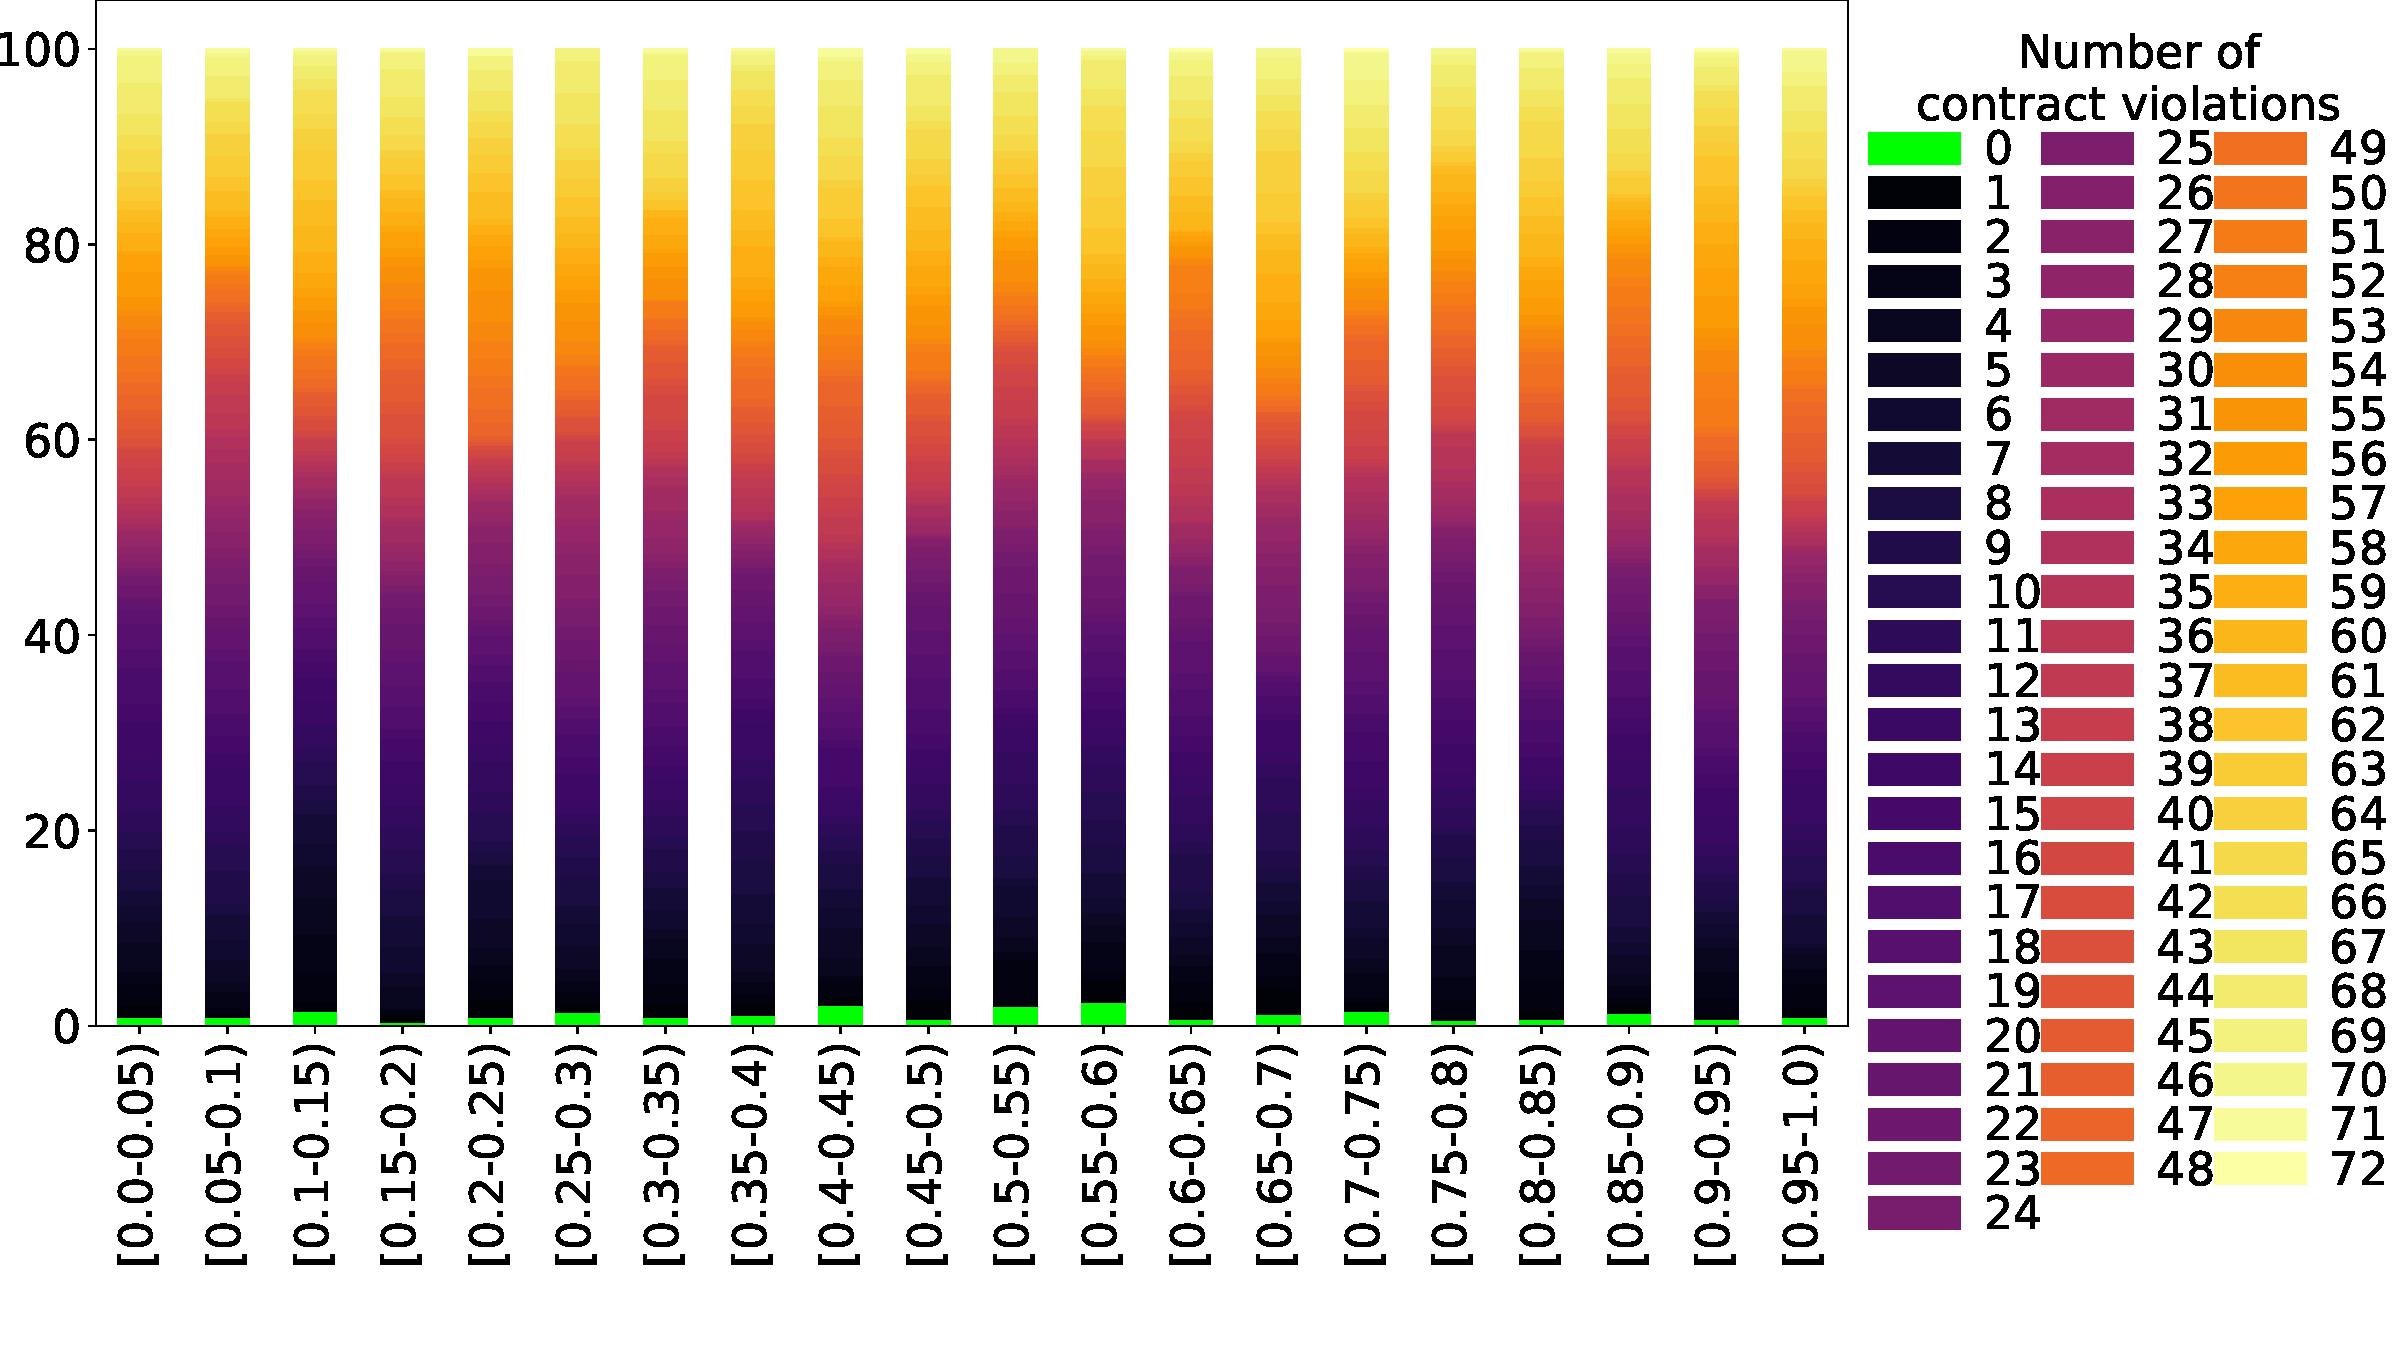
\includegraphics[width=\textwidth]{images/DistrValidityBig/evaluatorSoftwareValidityWeight.pdf}
	\caption[evaluatorSoftwareValidityWeight parameter values distribution for bigger problem]{evaluatorSoftwareValidityWeight parameter values distribution for bigger problem}
	\label{fig:evaluatorSoftwareValidityWeight_DistBig}
\end{figure}
\begin{figure}
	\centering
	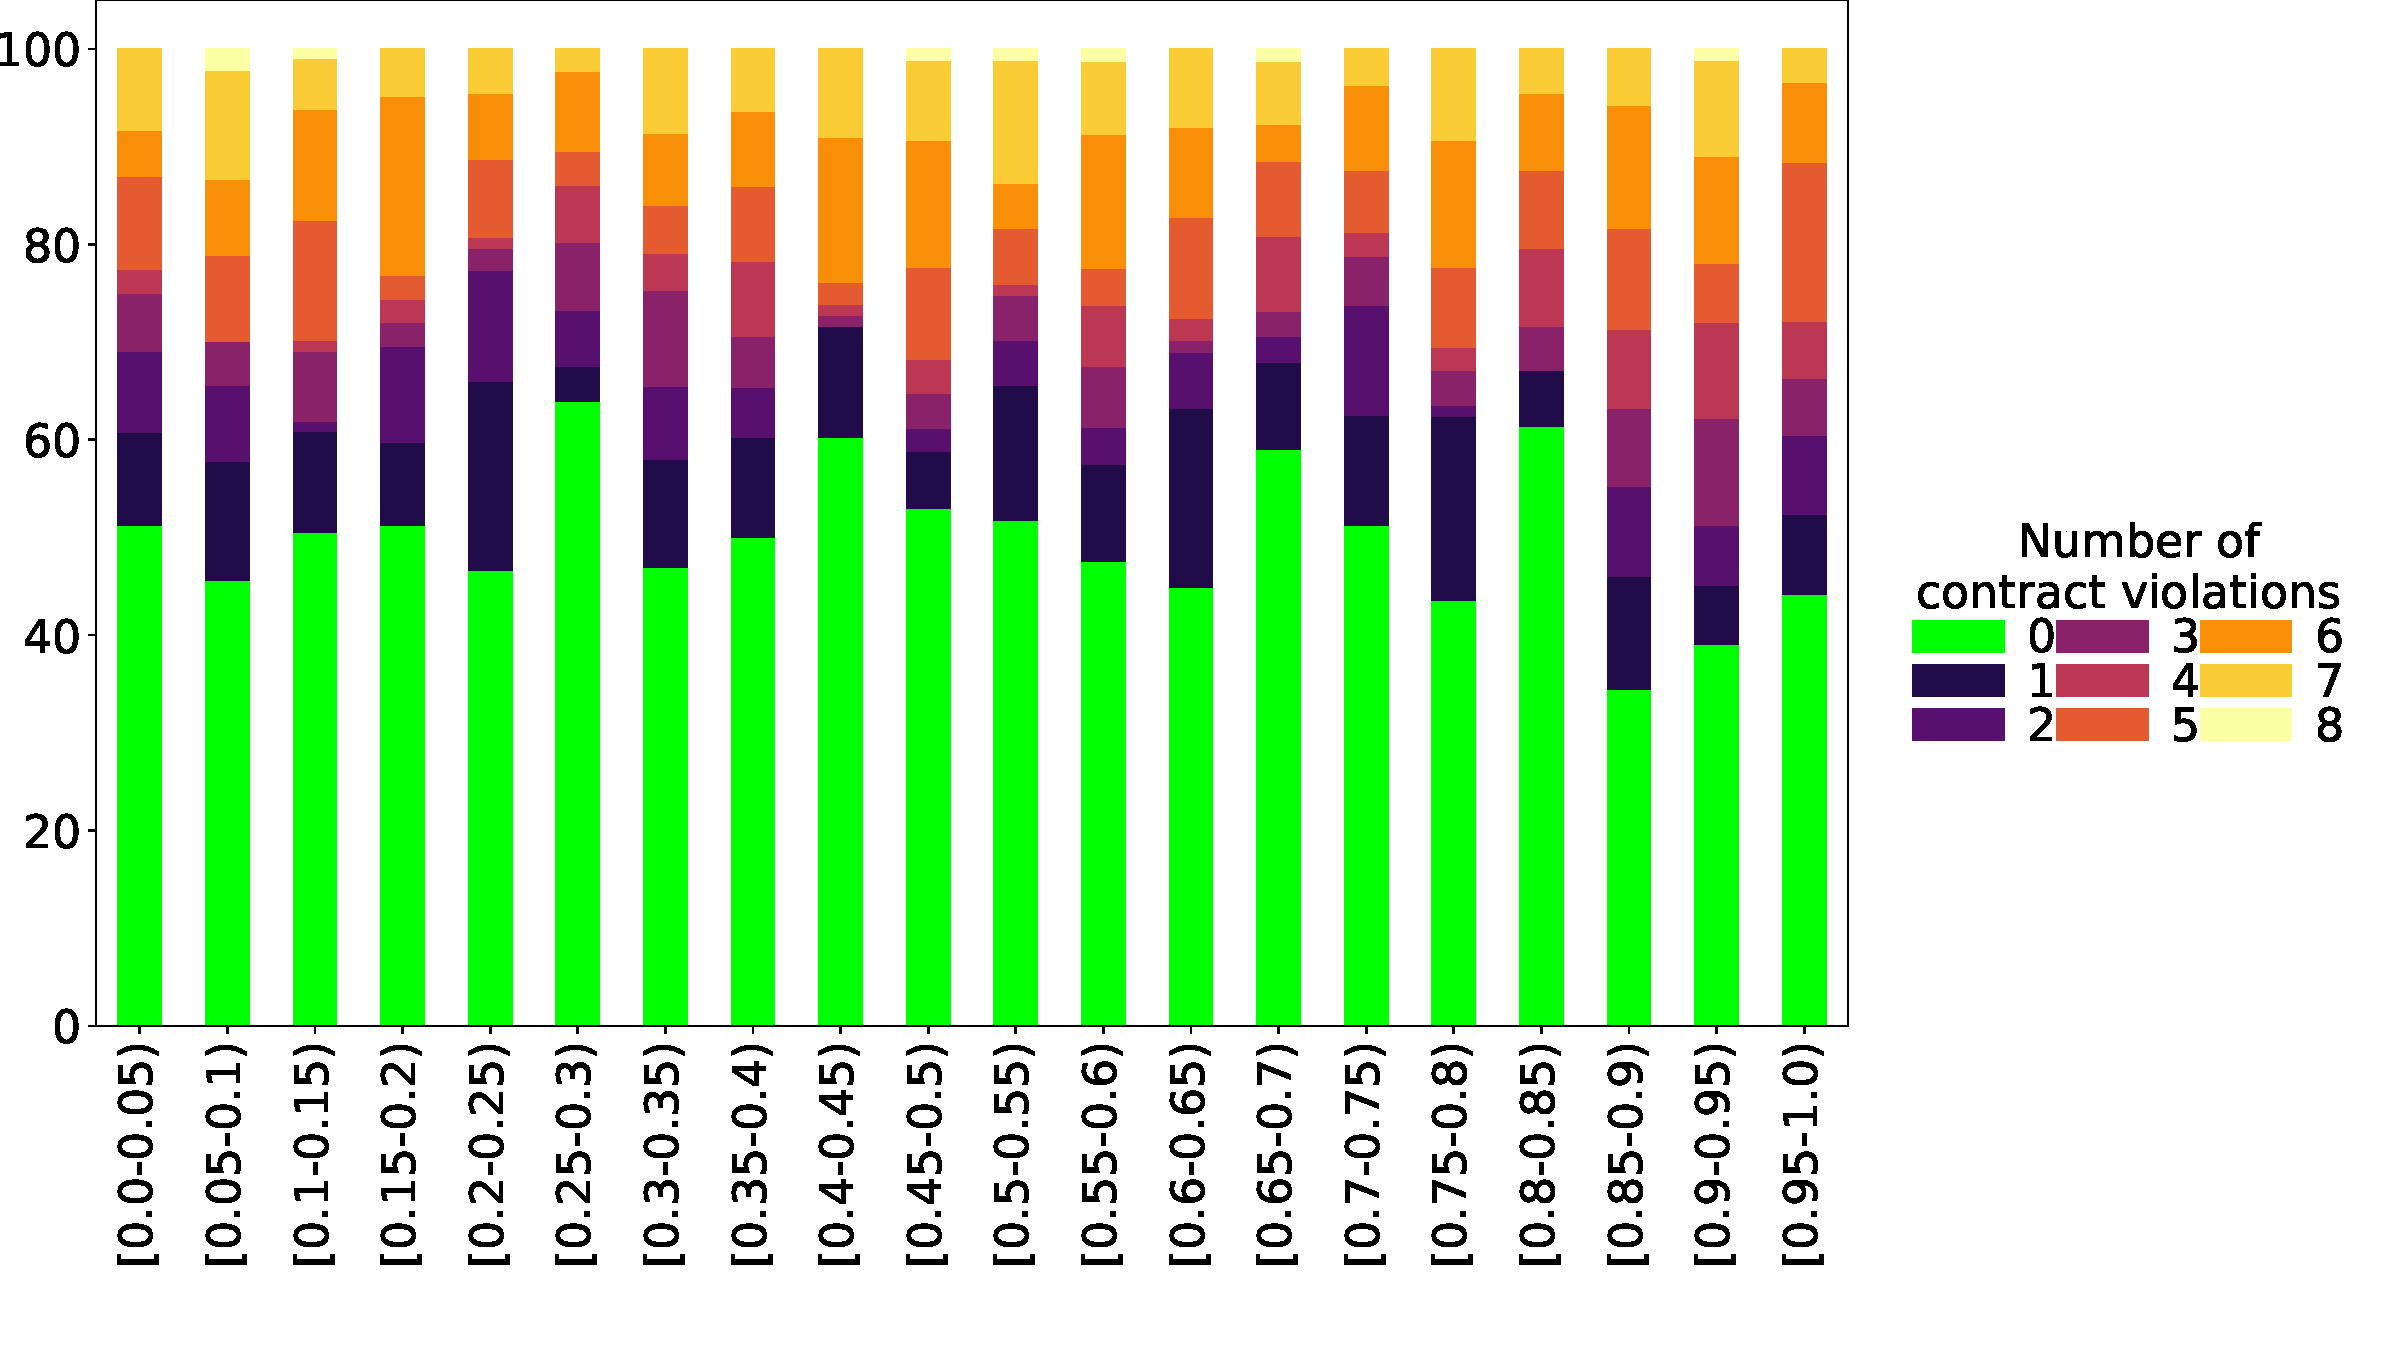
\includegraphics[width=\textwidth]{images/DistrValiditySmall/evaluatorSoftwareValidityWeight.pdf}
	\caption[evaluatorSoftwareValidityWeight parameter values distribution for smaller problem]{evaluatorSoftwareValidityWeight parameter values distribution for smaller problem}
	\label{fig:evaluatorSoftwareValidityWeight_DistSmall}
\end{figure}
\begin{figure}
	\centering
	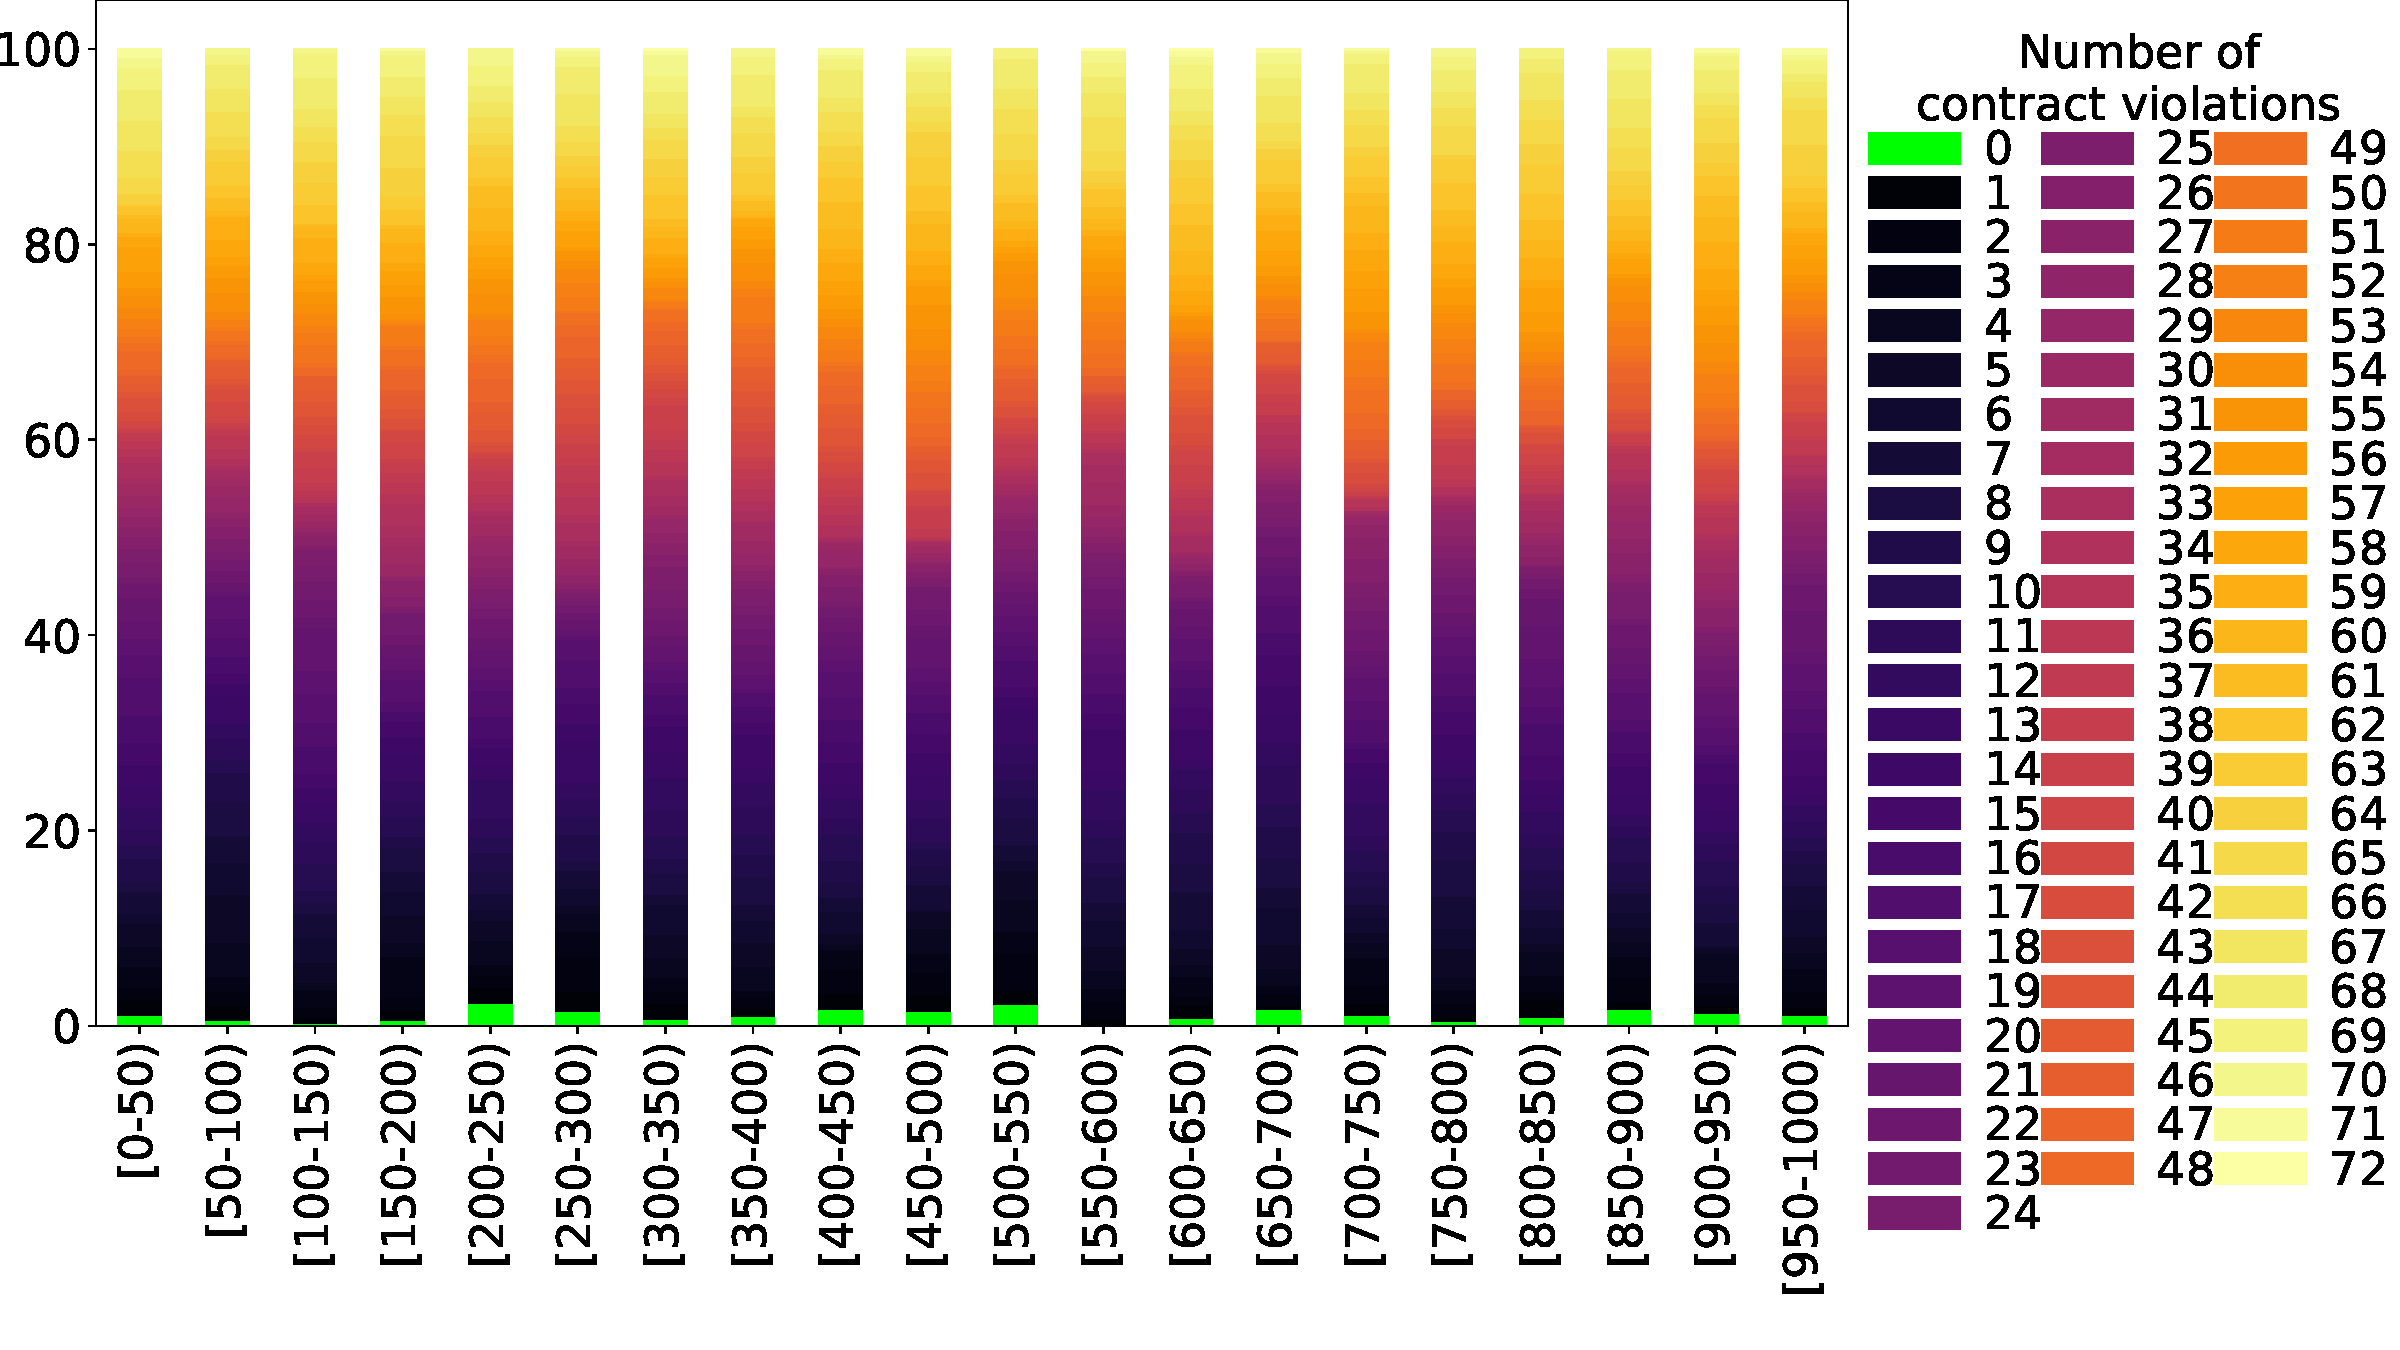
\includegraphics[width=\textwidth]{images/DistrValidityBig/randomSoftwareAssignmentAttempts.pdf}
	\caption[randomSoftwareAssignmentAttempts parameter values distribution for bigger problem]{randomSoftwareAssignmentAttempts parameter values distribution for bigger problem}
	\label{fig:randomSoftwareAssignmentAttempts_DistBig}
\end{figure}
\begin{figure}
	\centering
	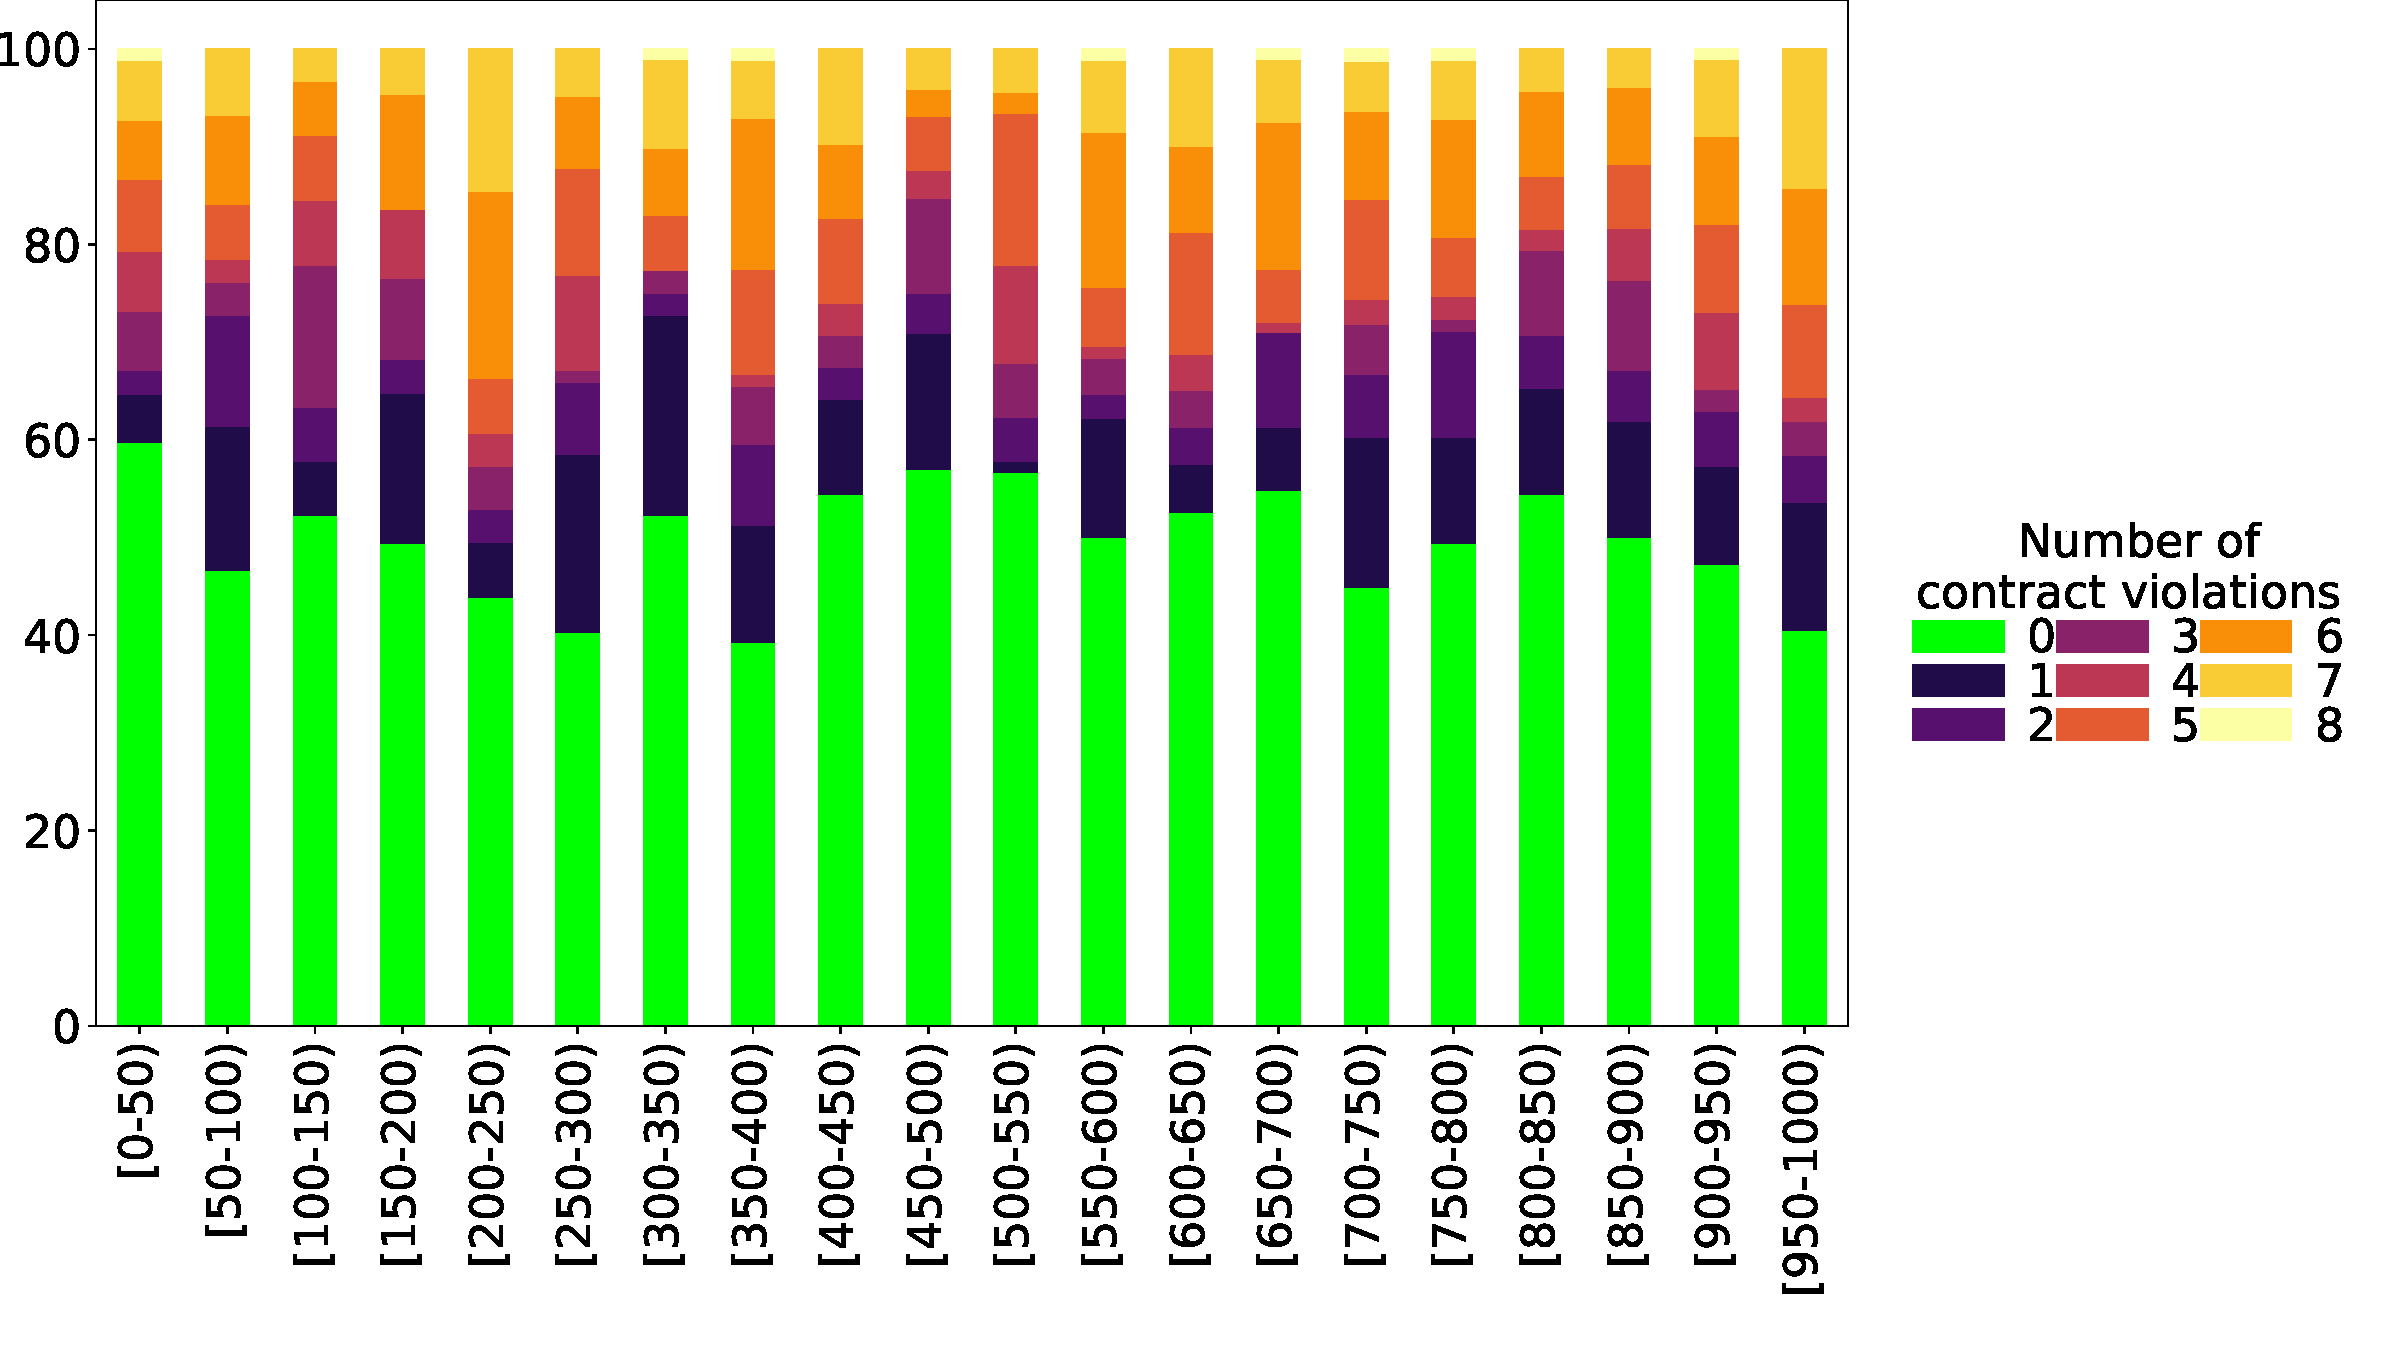
\includegraphics[width=\textwidth]{images/DistrValiditySmall/randomSoftwareAssignmentAttempts.pdf}
	\caption[randomSoftwareAssignmentAttempts parameter values distribution for smaller problem]{randomSoftwareAssignmentAttempts parameter values distribution for smaller problem}
	\label{fig:randomSoftwareAssignmentAttempts_DistSmall}
\end{figure}
\begin{figure}
	\centering
	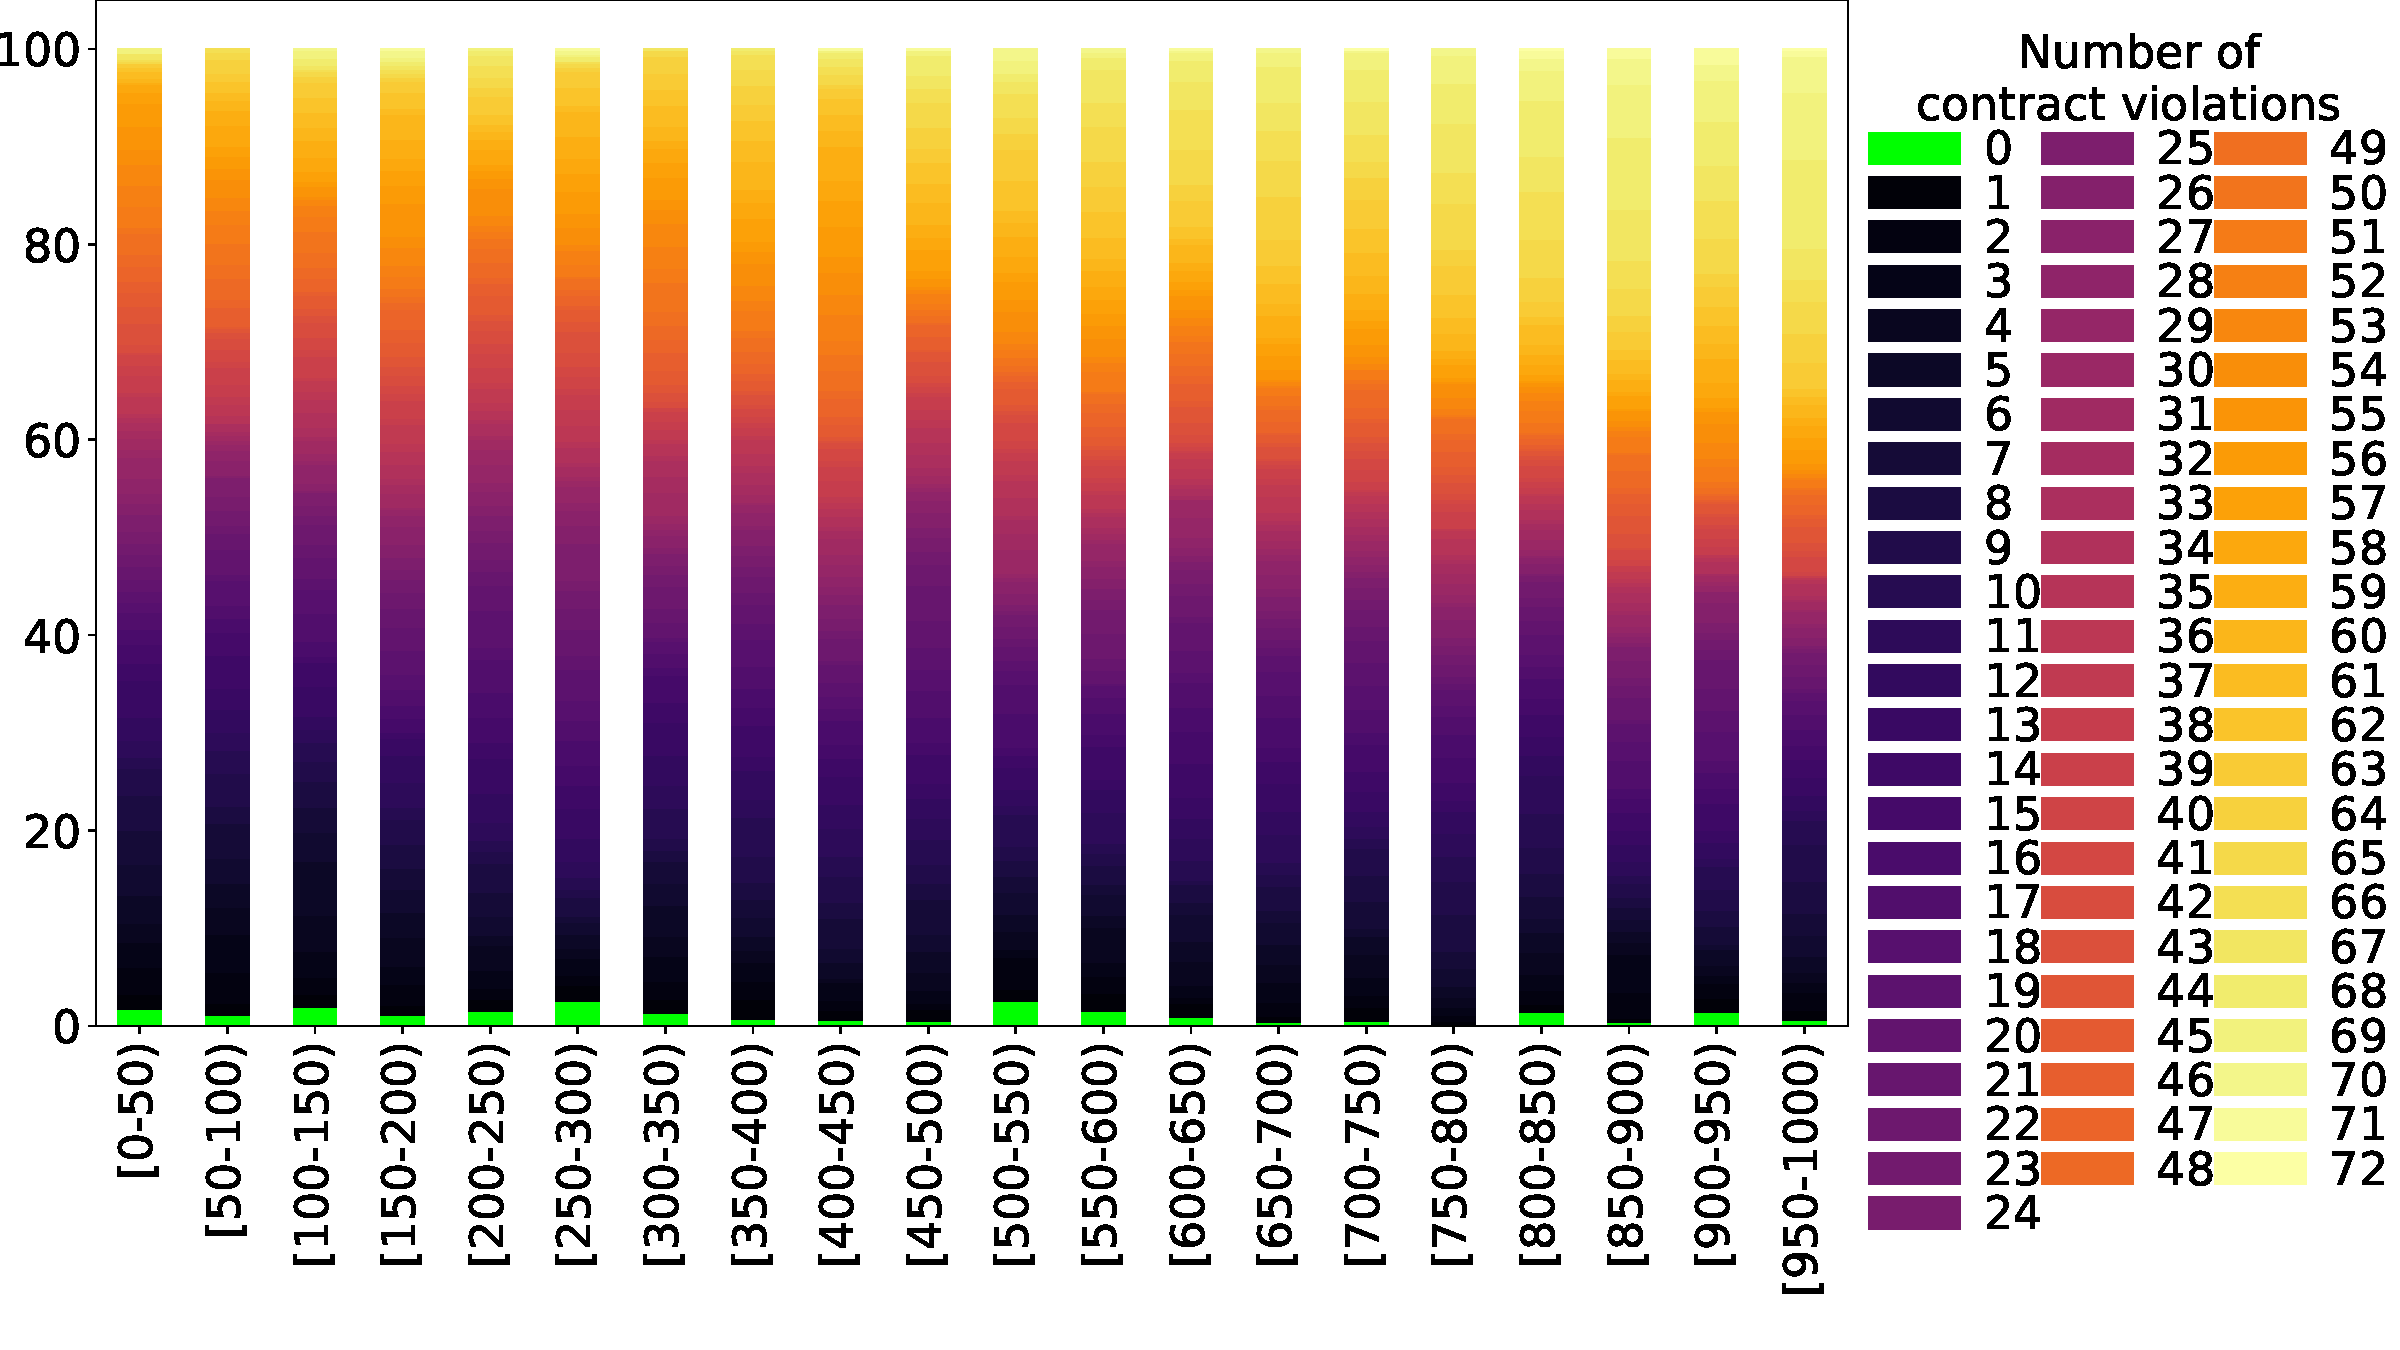
\includegraphics[width=\textwidth]{images/DistrValidityBig/populateSoftwareSolutionAttempts.pdf}
	\caption[populateSoftwareSolutionAttempts parameter values distribution for bigger problem]{populateSoftwareSolutionAttempts parameter values distribution for bigger problem}
	\label{fig:populateSoftwareSolutionAttempts_DistBig}
\end{figure}
\begin{figure}
	\centering
	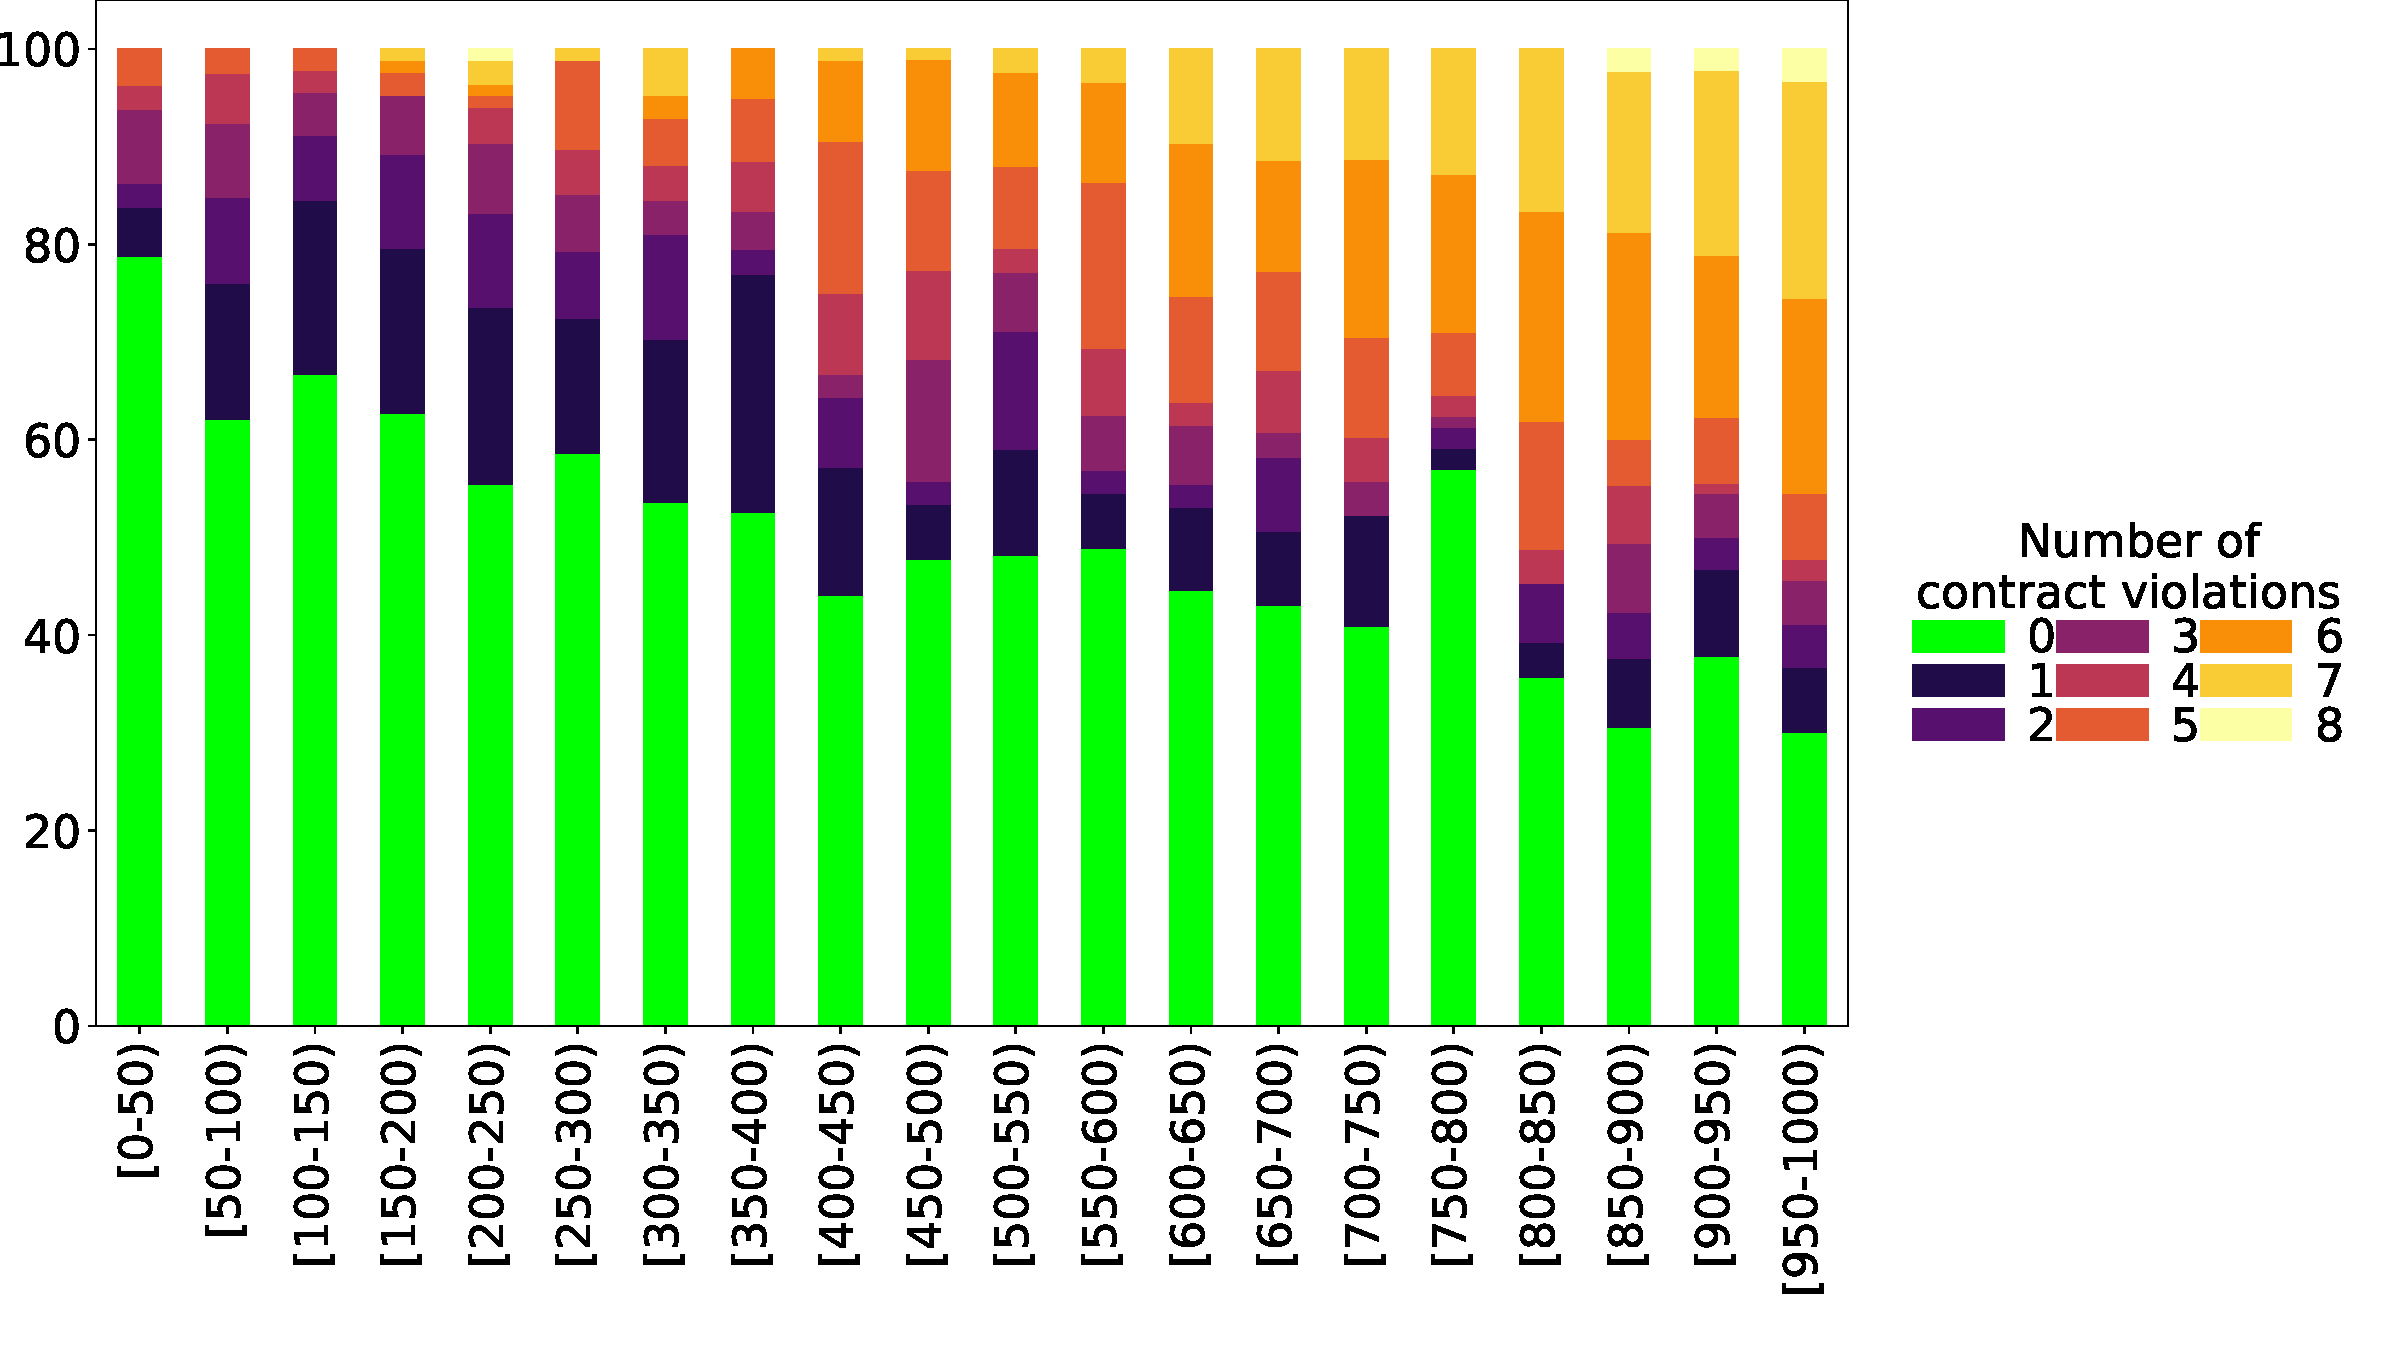
\includegraphics[width=\textwidth]{images/DistrValiditySmall/populateSoftwareSolutionAttempts.pdf}
	\caption[populateSoftwareSolutionAttempts parameter values distribution for smaller problem]{populateSoftwareSolutionAttempts parameter values distribution for smaller problem}
	\label{fig:populateSoftwareSolutionAttempts_DistSmall}
\end{figure}